%\pdfoutput=1
% Uncomment line above if submitting to arXiv and using pdflatex

% $Id: main.tex 73669 2015-06-05 10:36:06Z lafferty $
% ============================================================================
% Purpose: Template for LHCb documents
% Authors: Tomasz Skwarnicki, Roger Forty, Ulrik Egede
% Created on: 2010-09-24
% ============================================================================
\documentclass[12pt,a4paper]{article}
% For two column text, add "twocolumn" as an option to the document
% class. Also uncomment the two "onecolumn" and "twocolumn" lines
% around the title page below.

% Variables that controls behaviour
\usepackage{ifthen} % for conditional statements
\newboolean{pdflatex}
\setboolean{pdflatex}{true} % False for eps figures 

\newboolean{articletitles}
\setboolean{articletitles}{true} % False removes titles in references

\newboolean{uprightparticles}
\setboolean{uprightparticles}{false} %True for upright particle symbols

\newboolean{inbibliography}
\setboolean{inbibliography}{false} %True once you enter the bibliography


\usepackage{longtable} % only for template; not usually to be used in PAPERs
% THis file contains all the default packages and modifications for
% LHCb formatting

%% %%%%%%%%%%%%%%%%%%
%%  Page formatting
%% %%%%%%%%%%%%%%%%%%
\textheight=230mm
\textwidth=160mm
\oddsidemargin=7mm
\evensidemargin=-10mm
\topmargin=-10mm
\headsep=20mm
\columnsep=5mm
\addtolength{\belowcaptionskip}{0.5em}

\renewcommand{\textfraction}{0.01}
\renewcommand{\floatpagefraction}{0.99}
\renewcommand{\topfraction}{0.9}
\renewcommand{\bottomfraction}{0.9}


\setlength{\hoffset}{-2cm}
\setlength{\voffset}{-2cm}
% Page defaults ...
\topmargin=0.5cm
\oddsidemargin=2.5cm
\textwidth=16cm
\textheight=22cm
% Allow the page size to vary a bit ...
\raggedbottom
% To avoid Latex to be too fussy with line breaking ...
\sloppy

%% %%%%%%%%%%%%%%%%%%%%%%%
%% Packages to be used
%% %%%%%%%%%%%%%%%%%%%%%%% 
\usepackage{microtype}
\usepackage{lineno}  % for line numbering during review
\usepackage{xspace} % To avoid problems with missing or double spaces after
                    % predefined symbold
\usepackage{caption} %these three command get the figure and table captions automatically small
\renewcommand{\captionfont}{\small}
\renewcommand{\captionlabelfont}{\small}

%% Graphics
\usepackage{graphicx}  % to include figures (can also use other packages)
\usepackage{color}
\usepackage{colortbl}
\graphicspath{{./figs/}} % Make Latex search fig subdir for figures

%% Math
\usepackage{amsmath} % Adds a large collection of math symbols
\usepackage{amssymb}
\usepackage{amsfonts}
\usepackage{upgreek} % Adds in support for greek letters in roman typeset

%% fix to allow peaceful coexistence of line numbering and
%% mathematical objects
%% http://www.latex-community.org/forum/viewtopic.php?f=5&t=163
%%
\newcommand*\patchAmsMathEnvironmentForLineno[1]{%
\expandafter\let\csname old#1\expandafter\endcsname\csname #1\endcsname
\expandafter\let\csname oldend#1\expandafter\endcsname\csname
end#1\endcsname
 \renewenvironment{#1}%
   {\linenomath\csname old#1\endcsname}%
   {\csname oldend#1\endcsname\endlinenomath}%
}
\newcommand*\patchBothAmsMathEnvironmentsForLineno[1]{%
  \patchAmsMathEnvironmentForLineno{#1}%
  \patchAmsMathEnvironmentForLineno{#1*}%
}
\AtBeginDocument{%
\patchBothAmsMathEnvironmentsForLineno{equation}%
\patchBothAmsMathEnvironmentsForLineno{align}%
\patchBothAmsMathEnvironmentsForLineno{flalign}%
\patchBothAmsMathEnvironmentsForLineno{alignat}%
\patchBothAmsMathEnvironmentsForLineno{gather}%
\patchBothAmsMathEnvironmentsForLineno{multline}%
\patchBothAmsMathEnvironmentsForLineno{eqnarray}%
}

% Get hyperlinks to captions and in references.
% These do not work with revtex. Use "hypertext" as class option instead.
\usepackage{hyperref}    % Hyperlinks in references
\usepackage[all]{hypcap} % Internal hyperlinks to floats.

%%% $Id: lhcb-symbols-def.tex 74400 2015-06-18 12:45:24Z pkoppenb $
%%% ======================================================================
%%% Purpose: Standard LHCb aliases
%%% Author: Originally Ulrik Egede, adapted by Tomasz Skwarnicki for templates,
%%% rewritten by Chris Parkes
%%% Maintainer : Ulrik Egede (2010 - 2012)
%%% Maintainer : Rolf Oldeman (2012 - 2014)
%%% =======================================================================

%%% To use this file outside the normal LHCb document environment, the
%%% following should be added in a preamble (before \begin{document}
%%%
%%%\usepackage{ifthen} 
%%%\newboolean{uprightparticles}
%%%\setboolean{uprightparticles}{false} %Set true for upright particle symbols
%%% \usepackage{xspace} 
%%% \usepackage{upgreek}

%%%%%%%%%%%%%%%%%%%%%%%%%%%%%%%%%%%%%%%%%%%%%%%%%%%%%%%%%%%%
%%%
%%% The following is to ensure that the template automatically can process
%%% this file.
%%%
%%% Add comments with at least three %%% preceding.
%%% Add new sections with one % preceding
%%% Add new subsections with two %% preceding
%%%%%%%%%%%%%%%%%%%%%%%%%%%%%%%%%%%%%%%%%%%%%%%%%%%%%%%%%%%%

%%%%%%%%%%%%%
% Experiments
%%%%%%%%%%%%%
\def\lhcb {\mbox{LHCb}\xspace}
\def\atlas  {\mbox{ATLAS}\xspace}
\def\cms    {\mbox{CMS}\xspace}
\def\alice  {\mbox{ALICE}\xspace}
\def\babar  {\mbox{BaBar}\xspace}
\def\belle  {\mbox{Belle}\xspace}
\def\cleo   {\mbox{CLEO}\xspace}
\def\cdf    {\mbox{CDF}\xspace}
\def\dzero  {\mbox{D0}\xspace}
\def\aleph  {\mbox{ALEPH}\xspace}
\def\delphi {\mbox{DELPHI}\xspace}
\def\opal   {\mbox{OPAL}\xspace}
\def\lthree {\mbox{L3}\xspace}
\def\sld    {\mbox{SLD}\xspace}
%%%\def\argus  {\mbox{ARGUS}\xspace}
%%%\def\uaone  {\mbox{UA1}\xspace}
%%%\def\uatwo  {\mbox{UA2}\xspace}
%%%\def\ux85 {\mbox{UX85}\xspace}
\def\cern {\mbox{CERN}\xspace}
\def\lhc    {\mbox{LHC}\xspace}
\def\lep    {\mbox{LEP}\xspace}
\def\tevatron {Tevatron\xspace}

%% LHCb sub-detectors and sub-systems

%%%\def\pu     {PU\xspace}
\def\velo   {VELO\xspace}
\def\rich   {RICH\xspace}
\def\richone {RICH1\xspace}
\def\richtwo {RICH2\xspace}
\def\ttracker {TT\xspace}
\def\intr   {IT\xspace}
\def\st     {ST\xspace}
\def\ot     {OT\xspace}
%%%\def\Tone   {T1\xspace}
%%%\def\Ttwo   {T2\xspace}
%%%\def\Tthree {T3\xspace}
%%%\def\Mone   {M1\xspace}
%%%\def\Mtwo   {M2\xspace}
%%%\def\Mthree {M3\xspace}
%%%\def\Mfour  {M4\xspace}
%%%\def\Mfive  {M5\xspace}
\def\spd    {SPD\xspace}
\def\presh  {PS\xspace}
\def\ecal   {ECAL\xspace}
\def\hcal   {HCAL\xspace}
%%%\def\bcm    {BCM\xspace}
\def\MagUp {\mbox{\em Mag\kern -0.05em Up}\xspace}
\def\MagDown {\mbox{\em MagDown}\xspace}

%%%\def\ode    {ODE\xspace}
%%%\def\daq    {DAQ\xspace}
%%%\def\tfc    {TFC\xspace}
%%%\def\ecs    {ECS\xspace}
%%%\def\lone   {L0\xspace}
%%%\def\hlt    {HLT\xspace}
%%%\def\hltone {HLT1\xspace}
%%%\def\hlttwo {HLT2\xspace}

%%% Upright (not slanted) Particles

\ifthenelse{\boolean{uprightparticles}}%
{\def\Palpha      {\ensuremath{\upalpha}\xspace}
 \def\Pbeta       {\ensuremath{\upbeta}\xspace}
 \def\Pgamma      {\ensuremath{\upgamma}\xspace}                 
 \def\Pdelta      {\ensuremath{\updelta}\xspace}                 
 \def\Pepsilon    {\ensuremath{\upepsilon}\xspace}                 
 \def\Pvarepsilon {\ensuremath{\upvarepsilon}\xspace}                 
 \def\Pzeta       {\ensuremath{\upzeta}\xspace}                 
 \def\Peta        {\ensuremath{\upeta}\xspace}                 
 \def\Ptheta      {\ensuremath{\uptheta}\xspace}                 
 \def\Pvartheta   {\ensuremath{\upvartheta}\xspace}                 
 \def\Piota       {\ensuremath{\upiota}\xspace}                 
 \def\Pkappa      {\ensuremath{\upkappa}\xspace}                 
 \def\Plambda     {\ensuremath{\uplambda}\xspace}                 
 \def\Pmu         {\ensuremath{\upmu}\xspace}                 
 \def\Pnu         {\ensuremath{\upnu}\xspace}                 
 \def\Pxi         {\ensuremath{\upxi}\xspace}                 
 \def\Ppi         {\ensuremath{\uppi}\xspace}                 
 \def\Pvarpi      {\ensuremath{\upvarpi}\xspace}                 
 \def\Prho        {\ensuremath{\uprho}\xspace}                 
 \def\Pvarrho     {\ensuremath{\upvarrho}\xspace}                 
 \def\Ptau        {\ensuremath{\uptau}\xspace}                 
 \def\Pupsilon    {\ensuremath{\upupsilon}\xspace}                 
 \def\Pphi        {\ensuremath{\upphi}\xspace}                 
 \def\Pvarphi     {\ensuremath{\upvarphi}\xspace}                 
 \def\Pchi        {\ensuremath{\upchi}\xspace}                 
 \def\Ppsi        {\ensuremath{\uppsi}\xspace}                 
 \def\Pomega      {\ensuremath{\upomega}\xspace}                 

 \def\PDelta      {\ensuremath{\Delta}\xspace}                 
 \def\PXi      {\ensuremath{\Xi}\xspace}                 
 \def\PLambda      {\ensuremath{\Lambda}\xspace}                 
 \def\PSigma      {\ensuremath{\Sigma}\xspace}                 
 \def\POmega      {\ensuremath{\Omega}\xspace}                 
 \def\PUpsilon      {\ensuremath{\Upsilon}\xspace}                 
 
 %\mathchardef\Deltares="7101
 %\mathchardef\Xi="7104
 %\mathchardef\Lambda="7103
 %\mathchardef\Sigma="7106
 %\mathchardef\Omega="710A


 \def\PA      {\ensuremath{\mathrm{A}}\xspace}                 
 \def\PB      {\ensuremath{\mathrm{B}}\xspace}                 
 \def\PC      {\ensuremath{\mathrm{C}}\xspace}                 
 \def\PD      {\ensuremath{\mathrm{D}}\xspace}                 
 \def\PE      {\ensuremath{\mathrm{E}}\xspace}                 
 \def\PF      {\ensuremath{\mathrm{F}}\xspace}                 
 \def\PG      {\ensuremath{\mathrm{G}}\xspace}                 
 \def\PH      {\ensuremath{\mathrm{H}}\xspace}                 
 \def\PI      {\ensuremath{\mathrm{I}}\xspace}                 
 \def\PJ      {\ensuremath{\mathrm{J}}\xspace}                 
 \def\PK      {\ensuremath{\mathrm{K}}\xspace}                 
 \def\PL      {\ensuremath{\mathrm{L}}\xspace}                 
 \def\PM      {\ensuremath{\mathrm{M}}\xspace}                 
 \def\PN      {\ensuremath{\mathrm{N}}\xspace}                 
 \def\PO      {\ensuremath{\mathrm{O}}\xspace}                 
 \def\PP      {\ensuremath{\mathrm{P}}\xspace}                 
 \def\PQ      {\ensuremath{\mathrm{Q}}\xspace}                 
 \def\PR      {\ensuremath{\mathrm{R}}\xspace}                 
 \def\PS      {\ensuremath{\mathrm{S}}\xspace}                 
 \def\PT      {\ensuremath{\mathrm{T}}\xspace}                 
 \def\PU      {\ensuremath{\mathrm{U}}\xspace}                 
 \def\PV      {\ensuremath{\mathrm{V}}\xspace}                 
 \def\PW      {\ensuremath{\mathrm{W}}\xspace}                 
 \def\PX      {\ensuremath{\mathrm{X}}\xspace}                 
 \def\PY      {\ensuremath{\mathrm{Y}}\xspace}                 
 \def\PZ      {\ensuremath{\mathrm{Z}}\xspace}                 
 \def\Pa      {\ensuremath{\mathrm{a}}\xspace}                 
 \def\Pb      {\ensuremath{\mathrm{b}}\xspace}                 
 \def\Pc      {\ensuremath{\mathrm{c}}\xspace}                 
 \def\Pd      {\ensuremath{\mathrm{d}}\xspace}                 
 \def\Pe      {\ensuremath{\mathrm{e}}\xspace}                 
 \def\Pf      {\ensuremath{\mathrm{f}}\xspace}                 
 \def\Pg      {\ensuremath{\mathrm{g}}\xspace}                 
 \def\Ph      {\ensuremath{\mathrm{h}}\xspace}                 
 \def\Pi      {\ensuremath{\mathrm{i}}\xspace}                 
 \def\Pj      {\ensuremath{\mathrm{j}}\xspace}                 
 \def\Pk      {\ensuremath{\mathrm{k}}\xspace}                 
 \def\Pl      {\ensuremath{\mathrm{l}}\xspace}                 
 \def\Pm      {\ensuremath{\mathrm{m}}\xspace}                 
 \def\Pn      {\ensuremath{\mathrm{n}}\xspace}                 
 \def\Po      {\ensuremath{\mathrm{o}}\xspace}                 
 \def\Pp      {\ensuremath{\mathrm{p}}\xspace}                 
 \def\Pq      {\ensuremath{\mathrm{q}}\xspace}                 
 \def\Pr      {\ensuremath{\mathrm{r}}\xspace}                 
 \def\Ps      {\ensuremath{\mathrm{s}}\xspace}                 
 \def\Pt      {\ensuremath{\mathrm{t}}\xspace}                 
 \def\Pu      {\ensuremath{\mathrm{u}}\xspace}                 
 \def\Pv      {\ensuremath{\mathrm{v}}\xspace}                 
 \def\Pw      {\ensuremath{\mathrm{w}}\xspace}                 
 \def\Px      {\ensuremath{\mathrm{x}}\xspace}                 
 \def\Py      {\ensuremath{\mathrm{y}}\xspace}                 
 \def\Pz      {\ensuremath{\mathrm{z}}\xspace}                 
}
{\def\Palpha      {\ensuremath{\alpha}\xspace}
 \def\Pbeta       {\ensuremath{\beta}\xspace}
 \def\Pgamma      {\ensuremath{\gamma}\xspace}                 
 \def\Pdelta      {\ensuremath{\delta}\xspace}                 
 \def\Pepsilon    {\ensuremath{\epsilon}\xspace}                 
 \def\Pvarepsilon {\ensuremath{\varepsilon}\xspace}                 
 \def\Pzeta       {\ensuremath{\zeta}\xspace}                 
 \def\Peta        {\ensuremath{\eta}\xspace}                 
 \def\Ptheta      {\ensuremath{\theta}\xspace}                 
 \def\Pvartheta   {\ensuremath{\vartheta}\xspace}                 
 \def\Piota       {\ensuremath{\iota}\xspace}                 
 \def\Pkappa      {\ensuremath{\kappa}\xspace}                 
 \def\Plambda     {\ensuremath{\lambda}\xspace}                 
 \def\Pmu         {\ensuremath{\mu}\xspace}                 
 \def\Pnu         {\ensuremath{\nu}\xspace}                 
 \def\Pxi         {\ensuremath{\xi}\xspace}                 
 \def\Ppi         {\ensuremath{\pi}\xspace}                 
 \def\Pvarpi      {\ensuremath{\varpi}\xspace}                 
 \def\Prho        {\ensuremath{\rho}\xspace}                 
 \def\Pvarrho     {\ensuremath{\varrho}\xspace}                 
 \def\Ptau        {\ensuremath{\tau}\xspace}                 
 \def\Pupsilon    {\ensuremath{\upsilon}\xspace}                 
 \def\Pphi        {\ensuremath{\phi}\xspace}                 
 \def\Pvarphi     {\ensuremath{\varphi}\xspace}                 
 \def\Pchi        {\ensuremath{\chi}\xspace}                 
 \def\Ppsi        {\ensuremath{\psi}\xspace}                 
 \def\Pomega      {\ensuremath{\omega}\xspace}                 
 \mathchardef\PDelta="7101
 \mathchardef\PXi="7104
 \mathchardef\PLambda="7103
 \mathchardef\PSigma="7106
 \mathchardef\POmega="710A
 \mathchardef\PUpsilon="7107
 \def\PA      {\ensuremath{A}\xspace}                 
 \def\PB      {\ensuremath{B}\xspace}                 
 \def\PC      {\ensuremath{C}\xspace}                 
 \def\PD      {\ensuremath{D}\xspace}                 
 \def\PE      {\ensuremath{E}\xspace}                 
 \def\PF      {\ensuremath{F}\xspace}                 
 \def\PG      {\ensuremath{G}\xspace}                 
 \def\PH      {\ensuremath{H}\xspace}                 
 \def\PI      {\ensuremath{I}\xspace}                 
 \def\PJ      {\ensuremath{J}\xspace}                 
 \def\PK      {\ensuremath{K}\xspace}                 
 \def\PL      {\ensuremath{L}\xspace}                 
 \def\PM      {\ensuremath{M}\xspace}                 
 \def\PN      {\ensuremath{N}\xspace}                 
 \def\PO      {\ensuremath{O}\xspace}                 
 \def\PP      {\ensuremath{P}\xspace}                 
 \def\PQ      {\ensuremath{Q}\xspace}                 
 \def\PR      {\ensuremath{R}\xspace}                 
 \def\PS      {\ensuremath{S}\xspace}                 
 \def\PT      {\ensuremath{T}\xspace}                 
 \def\PU      {\ensuremath{U}\xspace}                 
 \def\PV      {\ensuremath{V}\xspace}                 
 \def\PW      {\ensuremath{W}\xspace}                 
 \def\PX      {\ensuremath{X}\xspace}                 
 \def\PY      {\ensuremath{Y}\xspace}                 
 \def\PZ      {\ensuremath{Z}\xspace}                 
 \def\Pa      {\ensuremath{a}\xspace}                 
 \def\Pb      {\ensuremath{b}\xspace}                 
 \def\Pc      {\ensuremath{c}\xspace}                 
 \def\Pd      {\ensuremath{d}\xspace}                 
 \def\Pe      {\ensuremath{e}\xspace}                 
 \def\Pf      {\ensuremath{f}\xspace}                 
 \def\Pg      {\ensuremath{g}\xspace}                 
 \def\Ph      {\ensuremath{h}\xspace}                 
 \def\Pi      {\ensuremath{i}\xspace}                 
 \def\Pj      {\ensuremath{j}\xspace}                 
 \def\Pk      {\ensuremath{k}\xspace}                 
 \def\Pl      {\ensuremath{l}\xspace}                 
 \def\Pm      {\ensuremath{m}\xspace}                 
 \def\Pn      {\ensuremath{n}\xspace}                 
 \def\Po      {\ensuremath{o}\xspace}                 
 \def\Pp      {\ensuremath{p}\xspace}                 
 \def\Pq      {\ensuremath{q}\xspace}                 
 \def\Pr      {\ensuremath{r}\xspace}                 
 \def\Ps      {\ensuremath{s}\xspace}                 
 \def\Pt      {\ensuremath{t}\xspace}                 
 \def\Pu      {\ensuremath{u}\xspace}                 
 \def\Pv      {\ensuremath{v}\xspace}                 
 \def\Pw      {\ensuremath{w}\xspace}                 
 \def\Px      {\ensuremath{x}\xspace}                 
 \def\Py      {\ensuremath{y}\xspace}                 
 \def\Pz      {\ensuremath{z}\xspace}                 
}

%%%%%%%%%%%%%%%%%%%%%%%%%%%%%%%%%%%%%%%%%%%%%%%
% Particles
\makeatletter
\ifcase \@ptsize \relax% 10pt
  \newcommand{\miniscule}{\@setfontsize\miniscule{4}{5}}% \tiny: 5/6
\or% 11pt
  \newcommand{\miniscule}{\@setfontsize\miniscule{5}{6}}% \tiny: 6/7
\or% 12pt
  \newcommand{\miniscule}{\@setfontsize\miniscule{5}{6}}% \tiny: 6/7
\fi
\makeatother


\DeclareRobustCommand{\optbar}[1]{\shortstack{{\miniscule (\rule[.5ex]{1.25em}{.18mm})}
  \\ [-.7ex] $#1$}}


%% Leptons

\let\emi\en
\def\electron   {{\ensuremath{\Pe}}\xspace}
\def\en         {{\ensuremath{\Pe^-}}\xspace}   % electron negative (\em is taken)
\def\ep         {{\ensuremath{\Pe^+}}\xspace}
\def\epm        {{\ensuremath{\Pe^\pm}}\xspace} 
\def\epem       {{\ensuremath{\Pe^+\Pe^-}}\xspace}
%%%\def\ee         {\ensuremath{\Pe^-\Pe^-}\xspace}

\def\muon       {{\ensuremath{\Pmu}}\xspace}
\def\mup        {{\ensuremath{\Pmu^+}}\xspace}
\def\mun        {{\ensuremath{\Pmu^-}}\xspace} % muon negative (\mum is taken)
\def\mumu       {{\ensuremath{\Pmu^+\Pmu^-}}\xspace}

\def\tauon      {{\ensuremath{\Ptau}}\xspace}
\def\taup       {{\ensuremath{\Ptau^+}}\xspace}
\def\taum       {{\ensuremath{\Ptau^-}}\xspace}
\def\tautau     {{\ensuremath{\Ptau^+\Ptau^-}}\xspace}

\def\lepton     {{\ensuremath{\ell}}\xspace}
\def\ellm       {{\ensuremath{\ell^-}}\xspace}
\def\ellp       {{\ensuremath{\ell^+}}\xspace}
%%%\def\ellell     {\ensuremath{\ell^+ \ell^-}\xspace}

\def\neu        {{\ensuremath{\Pnu}}\xspace}
\def\neub       {{\ensuremath{\overline{\Pnu}}}\xspace}
%%%\def\nuenueb    {\ensuremath{\neu\neub}\xspace}
\def\neue       {{\ensuremath{\neu_e}}\xspace}
\def\neueb      {{\ensuremath{\neub_e}}\xspace}
%%%\def\neueneueb  {\ensuremath{\neue\neueb}\xspace}
\def\neum       {{\ensuremath{\neu_\mu}}\xspace}
\def\neumb      {{\ensuremath{\neub_\mu}}\xspace}
%%%\def\neumneumb  {\ensuremath{\neum\neumb}\xspace}
\def\neut       {{\ensuremath{\neu_\tau}}\xspace}
\def\neutb      {{\ensuremath{\neub_\tau}}\xspace}
%%%\def\neutneutb  {\ensuremath{\neut\neutb}\xspace}
\def\neul       {{\ensuremath{\neu_\ell}}\xspace}
\def\neulb      {{\ensuremath{\neub_\ell}}\xspace}
%%%\def\neulneulb  {\ensuremath{\neul\neulb}\xspace}

%% Gauge bosons and scalars

\def\g      {{\ensuremath{\Pgamma}}\xspace}
\def\H      {{\ensuremath{\PH^0}}\xspace}
\def\Hp     {{\ensuremath{\PH^+}}\xspace}
\def\Hm     {{\ensuremath{\PH^-}}\xspace}
\def\Hpm    {{\ensuremath{\PH^\pm}}\xspace}
\def\W      {{\ensuremath{\PW}}\xspace}
\def\Wp     {{\ensuremath{\PW^+}}\xspace}
\def\Wm     {{\ensuremath{\PW^-}}\xspace}
\def\Wpm    {{\ensuremath{\PW^\pm}}\xspace}
\def\Z      {{\ensuremath{\PZ}}\xspace}

%% Quarks

\def\quark     {{\ensuremath{\Pq}}\xspace}
\def\quarkbar  {{\ensuremath{\overline \quark}}\xspace}
\def\qqbar     {{\ensuremath{\quark\quarkbar}}\xspace}
\def\uquark    {{\ensuremath{\Pu}}\xspace}
\def\uquarkbar {{\ensuremath{\overline \uquark}}\xspace}
\def\uubar     {{\ensuremath{\uquark\uquarkbar}}\xspace}
\def\dquark    {{\ensuremath{\Pd}}\xspace}
\def\dquarkbar {{\ensuremath{\overline \dquark}}\xspace}
\def\ddbar     {{\ensuremath{\dquark\dquarkbar}}\xspace}
\def\squark    {{\ensuremath{\Ps}}\xspace}
\def\squarkbar {{\ensuremath{\overline \squark}}\xspace}
\def\ssbar     {{\ensuremath{\squark\squarkbar}}\xspace}
\def\cquark    {{\ensuremath{\Pc}}\xspace}
\def\cquarkbar {{\ensuremath{\overline \cquark}}\xspace}
\def\ccbar     {{\ensuremath{\cquark\cquarkbar}}\xspace}
\def\bquark    {{\ensuremath{\Pb}}\xspace}
\def\bquarkbar {{\ensuremath{\overline \bquark}}\xspace}
\def\bbbar     {{\ensuremath{\bquark\bquarkbar}}\xspace}
\def\tquark    {{\ensuremath{\Pt}}\xspace}
\def\tquarkbar {{\ensuremath{\overline \tquark}}\xspace}
\def\ttbar     {{\ensuremath{\tquark\tquarkbar}}\xspace}

%% Light mesons

\def\hadron {{\ensuremath{\Ph}}\xspace}
\def\pion   {{\ensuremath{\Ppi}}\xspace}
\def\piz    {{\ensuremath{\pion^0}}\xspace}
\def\pizs   {{\ensuremath{\pion^0\mbox\,\rm{s}}}\xspace}
\def\pip    {{\ensuremath{\pion^+}}\xspace}
\def\pim    {{\ensuremath{\pion^-}}\xspace}
\def\pipm   {{\ensuremath{\pion^\pm}}\xspace}
\def\pimp   {{\ensuremath{\pion^\mp}}\xspace}

\def\rhomeson {{\ensuremath{\Prho}}\xspace}
\def\rhoz     {{\ensuremath{\rhomeson^0}}\xspace}
\def\rhop     {{\ensuremath{\rhomeson^+}}\xspace}
\def\rhom     {{\ensuremath{\rhomeson^-}}\xspace}
\def\rhopm    {{\ensuremath{\rhomeson^\pm}}\xspace}
\def\rhomp    {{\ensuremath{\rhomeson^\mp}}\xspace}

\def\kaon    {{\ensuremath{\PK}}\xspace}
%%% do NOT use ensuremath here
  \def\Kbar    {{\kern 0.2em\overline{\kern -0.2em \PK}{}}\xspace}
\def\Kb      {{\ensuremath{\Kbar}}\xspace}
\def\KorKbar    {\kern 0.18em\optbar{\kern -0.18em K}{}\xspace}
\def\Kz      {{\ensuremath{\kaon^0}}\xspace}
\def\Kzb     {{\ensuremath{\Kbar{}^0}}\xspace}
\def\Kp      {{\ensuremath{\kaon^+}}\xspace}
\def\Km      {{\ensuremath{\kaon^-}}\xspace}
\def\Kpm     {{\ensuremath{\kaon^\pm}}\xspace}
\def\Kmp     {{\ensuremath{\kaon^\mp}}\xspace}
\def\KS      {{\ensuremath{\kaon^0_{\rm\scriptscriptstyle S}}}\xspace}
\def\KL      {{\ensuremath{\kaon^0_{\rm\scriptscriptstyle L}}}\xspace}
\def\Kstarz  {{\ensuremath{\kaon^{*0}}}\xspace}
\def\Kstarzb {{\ensuremath{\Kbar{}^{*0}}}\xspace}
\def\Kstar   {{\ensuremath{\kaon^*}}\xspace}
\def\Kstarb  {{\ensuremath{\Kbar{}^*}}\xspace}
\def\Kstarp  {{\ensuremath{\kaon^{*+}}}\xspace}
\def\Kstarm  {{\ensuremath{\kaon^{*-}}}\xspace}
\def\Kstarpm {{\ensuremath{\kaon^{*\pm}}}\xspace}
\def\Kstarmp {{\ensuremath{\kaon^{*\mp}}}\xspace}

\newcommand{\etaz}{\ensuremath{\Peta}\xspace}
\newcommand{\etapr}{\ensuremath{\Peta^{\prime}}\xspace}
\newcommand{\phiz}{\ensuremath{\Pphi}\xspace}
\newcommand{\omegaz}{\ensuremath{\Pomega}\xspace}

%% Heavy mesons

%%% do NOT use ensuremath here
  \def\Dbar    {{\kern 0.2em\overline{\kern -0.2em \PD}{}}\xspace}
\def\D       {{\ensuremath{\PD}}\xspace}
\def\Db      {{\ensuremath{\Dbar}}\xspace}
\def\DorDbar    {\kern 0.18em\optbar{\kern -0.18em D}{}\xspace}
\def\Dz      {{\ensuremath{\D^0}}\xspace}
\def\Dzb     {{\ensuremath{\Dbar{}^0}}\xspace}
\def\Dp      {{\ensuremath{\D^+}}\xspace}
\def\Dm      {{\ensuremath{\D^-}}\xspace}
\def\Dpm     {{\ensuremath{\D^\pm}}\xspace}
\def\Dmp     {{\ensuremath{\D^\mp}}\xspace}
\def\Dstar   {{\ensuremath{\D^*}}\xspace}
\def\Dstarb  {{\ensuremath{\Dbar{}^*}}\xspace}
\def\Dstarz  {{\ensuremath{\D^{*0}}}\xspace}
\def\Dstarzb {{\ensuremath{\Dbar{}^{*0}}}\xspace}
\def\Dstarp  {{\ensuremath{\D^{*+}}}\xspace}
\def\Dstarm  {{\ensuremath{\D^{*-}}}\xspace}
\def\Dstarpm {{\ensuremath{\D^{*\pm}}}\xspace}
\def\Dstarmp {{\ensuremath{\D^{*\mp}}}\xspace}
\def\Ds      {{\ensuremath{\D^+_\squark}}\xspace}
\def\Dsp     {{\ensuremath{\D^+_\squark}}\xspace}
\def\Dsm     {{\ensuremath{\D^-_\squark}}\xspace}
\def\Dspm    {{\ensuremath{\D^{\pm}_\squark}}\xspace}
\def\Dsmp    {{\ensuremath{\D^{\mp}_\squark}}\xspace}
\def\Dss     {{\ensuremath{\D^{*+}_\squark}}\xspace}
\def\Dssp    {{\ensuremath{\D^{*+}_\squark}}\xspace}
\def\Dssm    {{\ensuremath{\D^{*-}_\squark}}\xspace}
\def\Dsspm   {{\ensuremath{\D^{*\pm}_\squark}}\xspace}
\def\Dssmp   {{\ensuremath{\D^{*\mp}_\squark}}\xspace}

\def\B       {{\ensuremath{\PB}}\xspace}
%%% do NOT use ensuremath here
\def\Bbar    {{\ensuremath{\kern 0.18em\overline{\kern -0.18em \PB}{}}}\xspace}
\def\Bb      {{\ensuremath{\Bbar}}\xspace}
\def\BorBbar    {\kern 0.18em\optbar{\kern -0.18em B}{}\xspace}
\def\Bz      {{\ensuremath{\B^0}}\xspace}
\def\Bzb     {{\ensuremath{\Bbar{}^0}}\xspace}
\def\Bu      {{\ensuremath{\B^+}}\xspace}
\def\Bub     {{\ensuremath{\B^-}}\xspace}
\def\Bp      {{\ensuremath{\Bu}}\xspace}
\def\Bm      {{\ensuremath{\Bub}}\xspace}
\def\Bpm     {{\ensuremath{\B^\pm}}\xspace}
\def\Bmp     {{\ensuremath{\B^\mp}}\xspace}
\def\Bd      {{\ensuremath{\B^0}}\xspace}
\def\Bs      {{\ensuremath{\B^0_\squark}}\xspace}
\def\Bsb     {{\ensuremath{\Bbar{}^0_\squark}}\xspace}
\def\Bdb     {{\ensuremath{\Bbar{}^0}}\xspace}
\def\Bc      {{\ensuremath{\B_\cquark^+}}\xspace}
\def\Bcp     {{\ensuremath{\B_\cquark^+}}\xspace}
\def\Bcm     {{\ensuremath{\B_\cquark^-}}\xspace}
\def\Bcpm    {{\ensuremath{\B_\cquark^\pm}}\xspace}

%% Onia

\def\jpsi     {{\ensuremath{{\PJ\mskip -3mu/\mskip -2mu\Ppsi\mskip 2mu}}}\xspace}
\def\psitwos  {{\ensuremath{\Ppsi{(2S)}}}\xspace}
\def\psiprpr  {{\ensuremath{\Ppsi(3770)}}\xspace}
\def\etac     {{\ensuremath{\Peta_\cquark}}\xspace}
\def\chiczero {{\ensuremath{\Pchi_{\cquark 0}}}\xspace}
\def\chicone  {{\ensuremath{\Pchi_{\cquark 1}}}\xspace}
\def\chictwo  {{\ensuremath{\Pchi_{\cquark 2}}}\xspace}
  %\mathchardef\Upsilon="7107
  \def\Y#1S{\ensuremath{\PUpsilon{(#1S)}}\xspace}% no space before {...}!
\def\OneS  {{\Y1S}}
\def\TwoS  {{\Y2S}}
\def\ThreeS{{\Y3S}}
\def\FourS {{\Y4S}}
\def\FiveS {{\Y5S}}

\def\chic  {{\ensuremath{\Pchi_{c}}}\xspace}

%% Baryons

\def\proton      {{\ensuremath{\Pp}}\xspace}
\def\antiproton  {{\ensuremath{\overline \proton}}\xspace}
\def\neutron     {{\ensuremath{\Pn}}\xspace}
\def\antineutron {{\ensuremath{\overline \neutron}}\xspace}
\def\Deltares    {{\ensuremath{\PDelta}}\xspace}
\def\Deltaresbar {{\ensuremath{\overline \Deltares}}\xspace}
\def\Xires       {{\ensuremath{\PXi}}\xspace}
\def\Xiresbar    {{\ensuremath{\overline \Xires}}\xspace}
\def\Lz          {{\ensuremath{\PLambda}}\xspace}
\def\Lbar        {{\ensuremath{\kern 0.1em\overline{\kern -0.1em\PLambda}}}\xspace}
\def\LorLbar    {\kern 0.18em\optbar{\kern -0.18em \PLambda}{}\xspace}
\def\Lambdares   {{\ensuremath{\PLambda}}\xspace}
\def\Lambdaresbar{{\ensuremath{\Lbar}}\xspace}
\def\Sigmares    {{\ensuremath{\PSigma}}\xspace}
\def\Sigmaresbar {{\ensuremath{\overline \Sigmares}}\xspace}
\def\Omegares    {{\ensuremath{\POmega}}\xspace}
\def\Omegaresbar {{\ensuremath{\overline \POmega}}\xspace}

%%% do NOT use ensuremath here
 % \def\Deltabar{\kern 0.25em\overline{\kern -0.25em \Deltares}{}\xspace}
 % \def\Sigbar{\kern 0.2em\overline{\kern -0.2em \Sigma}{}\xspace}
 % \def\Xibar{\kern 0.2em\overline{\kern -0.2em \Xi}{}\xspace}
 % \def\Obar{\kern 0.2em\overline{\kern -0.2em \Omega}{}\xspace}
 % \def\Nbar{\kern 0.2em\overline{\kern -0.2em N}{}\xspace}
 % \def\Xb{\kern 0.2em\overline{\kern -0.2em X}{}\xspace}

\def\Lb      {{\ensuremath{\Lz^0_\bquark}}\xspace}
\def\Lbbar   {{\ensuremath{\Lbar{}^0_\bquark}}\xspace}
\def\Lc      {{\ensuremath{\Lz^+_\cquark}}\xspace}
\def\Lcbar   {{\ensuremath{\Lbar{}^-_\cquark}}\xspace}
\def\Xib     {{\ensuremath{\Xires_\bquark}}\xspace}
\def\Xibz    {{\ensuremath{\Xires^0_\bquark}}\xspace}
\def\Xibm    {{\ensuremath{\Xires^-_\bquark}}\xspace}
\def\Xibbar  {{\ensuremath{\Xiresbar{}_\bquark}}\xspace}
\def\Xibbarz {{\ensuremath{\Xiresbar{}_\bquark^0}}\xspace}
\def\Xibbarp {{\ensuremath{\Xiresbar{}_\bquark^+}}\xspace}
\def\Xic     {{\ensuremath{\Xires_\cquark}}\xspace}
\def\Xicz    {{\ensuremath{\Xires^0_\cquark}}\xspace}
\def\Xicp    {{\ensuremath{\Xires^+_\cquark}}\xspace}
\def\Xicbar  {{\ensuremath{\Xiresbar{}_\cquark}}\xspace}
\def\Xicbarz {{\ensuremath{\Xiresbar{}_\cquark^0}}\xspace}
\def\Xicbarm {{\ensuremath{\Xiresbar{}_\cquark^-}}\xspace}
\def\Omegac    {{\ensuremath{\Omegares^0_\cquark}}\xspace}
\def\Omegacbar {{\ensuremath{\Omegaresbar{}_\cquark^0}}\xspace}
\def\Omegab    {{\ensuremath{\Omegares^-_\bquark}}\xspace}
\def\Omegabbar {{\ensuremath{\Omegaresbar{}_\bquark^+}}\xspace}

%%%%%%%%%%%%%%%%%%
% Physics symbols
%%%%%%%%%%%%%%%%%

%% Decays
\def\BF         {{\ensuremath{\cal B}}\xspace}
\def\BRvis      {{\ensuremath{\BR_{\rm{vis}}}}}
\def\BR         {\BF}
\newcommand{\decay}[2]{\ensuremath{#1\!\to #2}\xspace}         % {\Pa}{\Pb \Pc}
\def\ra                 {\ensuremath{\rightarrow}\xspace}
\def\to                 {\ensuremath{\rightarrow}\xspace}

%% Lifetimes
\newcommand{\tauBs}{{\ensuremath{\tau_{\Bs}}}\xspace}
\newcommand{\tauBd}{{\ensuremath{\tau_{\Bd}}}\xspace}
\newcommand{\tauBz}{{\ensuremath{\tau_{\Bz}}}\xspace}
\newcommand{\tauBu}{{\ensuremath{\tau_{\Bp}}}\xspace}
\newcommand{\tauDp}{{\ensuremath{\tau_{\Dp}}}\xspace}
\newcommand{\tauDz}{{\ensuremath{\tau_{\Dz}}}\xspace}
\newcommand{\tauL}{{\ensuremath{\tau_{\rm L}}}\xspace}
\newcommand{\tauH}{{\ensuremath{\tau_{\rm H}}}\xspace}

%% Masses
\newcommand{\mBd}{{\ensuremath{m_{\Bd}}}\xspace}
\newcommand{\mBp}{{\ensuremath{m_{\Bp}}}\xspace}
\newcommand{\mBs}{{\ensuremath{m_{\Bs}}}\xspace}
\newcommand{\mBc}{{\ensuremath{m_{\Bc}}}\xspace}
\newcommand{\mLb}{{\ensuremath{m_{\Lb}}}\xspace}

%% EW theory, groups
\def\grpsuthree {{\ensuremath{\mathrm{SU}(3)}}\xspace}
\def\grpsutw    {{\ensuremath{\mathrm{SU}(2)}}\xspace}
\def\grpuone    {{\ensuremath{\mathrm{U}(1)}}\xspace}

\def\ssqtw   {{\ensuremath{\sin^{2}\!\theta_{\mathrm{W}}}}\xspace}
\def\csqtw   {{\ensuremath{\cos^{2}\!\theta_{\mathrm{W}}}}\xspace}
\def\stw     {{\ensuremath{\sin\theta_{\mathrm{W}}}}\xspace}
\def\ctw     {{\ensuremath{\cos\theta_{\mathrm{W}}}}\xspace}
\def\ssqtwef {{\ensuremath{{\sin}^{2}\theta_{\mathrm{W}}^{\mathrm{eff}}}}\xspace}
\def\csqtwef {{\ensuremath{{\cos}^{2}\theta_{\mathrm{W}}^{\mathrm{eff}}}}\xspace}
\def\stwef   {{\ensuremath{\sin\theta_{\mathrm{W}}^{\mathrm{eff}}}}\xspace}
\def\ctwef   {{\ensuremath{\cos\theta_{\mathrm{W}}^{\mathrm{eff}}}}\xspace}
\def\gv      {{\ensuremath{g_{\mbox{\tiny V}}}}\xspace}
\def\ga      {{\ensuremath{g_{\mbox{\tiny A}}}}\xspace}

\def\order   {{\ensuremath{\mathcal{O}}}\xspace}
\def\ordalph {{\ensuremath{\mathcal{O}(\alpha)}}\xspace}
\def\ordalsq {{\ensuremath{\mathcal{O}(\alpha^{2})}}\xspace}
\def\ordalcb {{\ensuremath{\mathcal{O}(\alpha^{3})}}\xspace}

%% QCD parameters
\newcommand{\as}{{\ensuremath{\alpha_s}}\xspace}
\newcommand{\MSb}{{\ensuremath{\overline{\mathrm{MS}}}}\xspace}
\newcommand{\lqcd}{{\ensuremath{\Lambda_{\mathrm{QCD}}}}\xspace}
\def\qsq       {{\ensuremath{q^2}}\xspace}

%% CKM, CP violation

\def\eps   {{\ensuremath{\varepsilon}}\xspace}
\def\epsK  {{\ensuremath{\varepsilon_K}}\xspace}
\def\epsB  {{\ensuremath{\varepsilon_B}}\xspace}
\def\epsp  {{\ensuremath{\varepsilon^\prime_K}}\xspace}

\def\CP                {{\ensuremath{C\!P}}\xspace}
\def\CPT               {{\ensuremath{C\!PT}}\xspace}

\def\rhobar {{\ensuremath{\overline \rho}}\xspace}
\def\etabar {{\ensuremath{\overline \eta}}\xspace}

\def\Vud  {{\ensuremath{V_{\uquark\dquark}}}\xspace}
\def\Vcd  {{\ensuremath{V_{\cquark\dquark}}}\xspace}
\def\Vtd  {{\ensuremath{V_{\tquark\dquark}}}\xspace}
\def\Vus  {{\ensuremath{V_{\uquark\squark}}}\xspace}
\def\Vcs  {{\ensuremath{V_{\cquark\squark}}}\xspace}
\def\Vts  {{\ensuremath{V_{\tquark\squark}}}\xspace}
\def\Vub  {{\ensuremath{V_{\uquark\bquark}}}\xspace}
\def\Vcb  {{\ensuremath{V_{\cquark\bquark}}}\xspace}
\def\Vtb  {{\ensuremath{V_{\tquark\bquark}}}\xspace}
\def\Vuds  {{\ensuremath{V_{\uquark\dquark}^\ast}}\xspace}
\def\Vcds  {{\ensuremath{V_{\cquark\dquark}^\ast}}\xspace}
\def\Vtds  {{\ensuremath{V_{\tquark\dquark}^\ast}}\xspace}
\def\Vuss  {{\ensuremath{V_{\uquark\squark}^\ast}}\xspace}
\def\Vcss  {{\ensuremath{V_{\cquark\squark}^\ast}}\xspace}
\def\Vtss  {{\ensuremath{V_{\tquark\squark}^\ast}}\xspace}
\def\Vubs  {{\ensuremath{V_{\uquark\bquark}^\ast}}\xspace}
\def\Vcbs  {{\ensuremath{V_{\cquark\bquark}^\ast}}\xspace}
\def\Vtbs  {{\ensuremath{V_{\tquark\bquark}^\ast}}\xspace}

%% Oscillations

\newcommand{\dm}{{\ensuremath{\Delta m}}\xspace}
\newcommand{\dms}{{\ensuremath{\Delta m_{\squark}}}\xspace}
\newcommand{\dmd}{{\ensuremath{\Delta m_{\dquark}}}\xspace}
\newcommand{\DG}{{\ensuremath{\Delta\Gamma}}\xspace}
\newcommand{\DGs}{{\ensuremath{\Delta\Gamma_{\squark}}}\xspace}
\newcommand{\DGd}{{\ensuremath{\Delta\Gamma_{\dquark}}}\xspace}
\newcommand{\Gs}{{\ensuremath{\Gamma_{\squark}}}\xspace}
\newcommand{\Gd}{{\ensuremath{\Gamma_{\dquark}}}\xspace}
\newcommand{\MBq}{{\ensuremath{M_{\B_\quark}}}\xspace}
\newcommand{\DGq}{{\ensuremath{\Delta\Gamma_{\quark}}}\xspace}
\newcommand{\Gq}{{\ensuremath{\Gamma_{\quark}}}\xspace}
\newcommand{\dmq}{{\ensuremath{\Delta m_{\quark}}}\xspace}
\newcommand{\GL}{{\ensuremath{\Gamma_{\rm L}}}\xspace}
\newcommand{\GH}{{\ensuremath{\Gamma_{\rm H}}}\xspace}
\newcommand{\DGsGs}{{\ensuremath{\Delta\Gamma_{\squark}/\Gamma_{\squark}}}\xspace}
\newcommand{\Delm}{{\mbox{$\Delta m $}}\xspace}
\newcommand{\ACP}{{\ensuremath{{\cal A}^{\CP}}}\xspace}
\newcommand{\Adir}{{\ensuremath{{\cal A}^{\rm dir}}}\xspace}
\newcommand{\Amix}{{\ensuremath{{\cal A}^{\rm mix}}}\xspace}
\newcommand{\ADelta}{{\ensuremath{{\cal A}^\Delta}}\xspace}
\newcommand{\phid}{{\ensuremath{\phi_{\dquark}}}\xspace}
\newcommand{\sinphid}{{\ensuremath{\sin\!\phid}}\xspace}
\newcommand{\phis}{{\ensuremath{\phi_{\squark}}}\xspace}
\newcommand{\betas}{{\ensuremath{\beta_{\squark}}}\xspace}
\newcommand{\sbetas}{{\ensuremath{\sigma(\beta_{\squark})}}\xspace}
\newcommand{\stbetas}{{\ensuremath{\sigma(2\beta_{\squark})}}\xspace}
\newcommand{\stphis}{{\ensuremath{\sigma(\phi_{\squark})}}\xspace}
\newcommand{\sinphis}{{\ensuremath{\sin\!\phis}}\xspace}

%% Tagging
\newcommand{\edet}{{\ensuremath{\varepsilon_{\rm det}}}\xspace}
\newcommand{\erec}{{\ensuremath{\varepsilon_{\rm rec/det}}}\xspace}
\newcommand{\esel}{{\ensuremath{\varepsilon_{\rm sel/rec}}}\xspace}
\newcommand{\etrg}{{\ensuremath{\varepsilon_{\rm trg/sel}}}\xspace}
\newcommand{\etot}{{\ensuremath{\varepsilon_{\rm tot}}}\xspace}

\newcommand{\mistag}{\ensuremath{\omega}\xspace}
\newcommand{\wcomb}{\ensuremath{\omega^{\rm comb}}\xspace}
\newcommand{\etag}{{\ensuremath{\varepsilon_{\rm tag}}}\xspace}
\newcommand{\etagcomb}{{\ensuremath{\varepsilon_{\rm tag}^{\rm comb}}}\xspace}
\newcommand{\effeff}{\ensuremath{\varepsilon_{\rm eff}}\xspace}
\newcommand{\effeffcomb}{\ensuremath{\varepsilon_{\rm eff}^{\rm comb}}\xspace}
\newcommand{\efftag}{{\ensuremath{\etag(1-2\omega)^2}}\xspace}
\newcommand{\effD}{{\ensuremath{\etag D^2}}\xspace}

\newcommand{\etagprompt}{{\ensuremath{\varepsilon_{\rm tag}^{\rm Pr}}}\xspace}
\newcommand{\etagLL}{{\ensuremath{\varepsilon_{\rm tag}^{\rm LL}}}\xspace}

%% Key decay channels

\def\BdToKstmm    {\decay{\Bd}{\Kstarz\mup\mun}}
\def\BdbToKstmm   {\decay{\Bdb}{\Kstarzb\mup\mun}}

\def\BsToJPsiPhi  {\decay{\Bs}{\jpsi\phi}}
\def\BdToJPsiKst  {\decay{\Bd}{\jpsi\Kstarz}}
\def\BdbToJPsiKst {\decay{\Bdb}{\jpsi\Kstarzb}}

\def\BsPhiGam     {\decay{\Bs}{\phi \g}}
\def\BdKstGam     {\decay{\Bd}{\Kstarz \g}}

\def\BTohh        {\decay{\B}{\Ph^+ \Ph'^-}}
\def\BdTopipi     {\decay{\Bd}{\pip\pim}}
\def\BdToKpi      {\decay{\Bd}{\Kp\pim}}
\def\BsToKK       {\decay{\Bs}{\Kp\Km}}
\def\BsTopiK      {\decay{\Bs}{\pip\Km}}

%% Rare decays
\def\BdKstee  {\decay{\Bd}{\Kstarz\epem}}
\def\BdbKstee {\decay{\Bdb}{\Kstarzb\epem}}
\def\bsll     {\decay{\bquark}{\squark \ell^+ \ell^-}}
\def\AFB      {\ensuremath{A_{\mathrm{FB}}}\xspace}
\def\FL       {\ensuremath{F_{\mathrm{L}}}\xspace}
\def\AT#1     {\ensuremath{A_{\mathrm{T}}^{#1}}\xspace}           % 2
\def\btosgam  {\decay{\bquark}{\squark \g}}
\def\btodgam  {\decay{\bquark}{\dquark \g}}
\def\Bsmm     {\decay{\Bs}{\mup\mun}}
\def\Bdmm     {\decay{\Bd}{\mup\mun}}
\def\ctl       {\ensuremath{\cos{\theta_\ell}}\xspace}
\def\ctk       {\ensuremath{\cos{\theta_K}}\xspace}

%% Wilson coefficients and operators
\def\C#1      {\ensuremath{\mathcal{C}_{#1}}\xspace}                       % 9
\def\Cp#1     {\ensuremath{\mathcal{C}_{#1}^{'}}\xspace}                    % 7
\def\Ceff#1   {\ensuremath{\mathcal{C}_{#1}^{\mathrm{(eff)}}}\xspace}        % 9  
\def\Cpeff#1  {\ensuremath{\mathcal{C}_{#1}^{'\mathrm{(eff)}}}\xspace}       % 7
\def\Ope#1    {\ensuremath{\mathcal{O}_{#1}}\xspace}                       % 2
\def\Opep#1   {\ensuremath{\mathcal{O}_{#1}^{'}}\xspace}                    % 7

%% Charm

\def\xprime     {\ensuremath{x^{\prime}}\xspace}
\def\yprime     {\ensuremath{y^{\prime}}\xspace}
\def\ycp        {\ensuremath{y_{\CP}}\xspace}
\def\agamma     {\ensuremath{A_{\Gamma}}\xspace}
%%%\def\kpi        {\ensuremath{\PK\Ppi}\xspace}
%%%\def\kk         {\ensuremath{\PK\PK}\xspace}
%%%\def\dkpi       {\decay{\PD}{\PK\Ppi}}
%%%\def\dkk        {\decay{\PD}{\PK\PK}}
\def\dkpicf     {\decay{\Dz}{\Km\pip}}

%% QM
\newcommand{\bra}[1]{\ensuremath{\langle #1|}}             % {a}
\newcommand{\ket}[1]{\ensuremath{|#1\rangle}}              % {b}
\newcommand{\braket}[2]{\ensuremath{\langle #1|#2\rangle}} % {a}{b}

%%%%%%%%%%%%%%%%%%%%%%%%%%%%%%%%%%%%%%%%%%%%%%%%%%
% Units
%%%%%%%%%%%%%%%%%%%%%%%%%%%%%%%%%%%%%%%%%%%%%%%%%%
\newcommand{\unit}[1]{\ensuremath{\rm\,#1}\xspace}          % {kg}

%% Energy and momentum
\newcommand{\tev}{\ifthenelse{\boolean{inbibliography}}{\ensuremath{~T\kern -0.05em eV}\xspace}{\ensuremath{\mathrm{\,Te\kern -0.1em V}}}\xspace}
\newcommand{\gev}{\ensuremath{\mathrm{\,Ge\kern -0.1em V}}\xspace}
\newcommand{\mev}{\ensuremath{\mathrm{\,Me\kern -0.1em V}}\xspace}
\newcommand{\kev}{\ensuremath{\mathrm{\,ke\kern -0.1em V}}\xspace}
\newcommand{\ev}{\ensuremath{\mathrm{\,e\kern -0.1em V}}\xspace}
\newcommand{\gevc}{\ensuremath{{\mathrm{\,Ge\kern -0.1em V\!/}c}}\xspace}
\newcommand{\mevc}{\ensuremath{{\mathrm{\,Me\kern -0.1em V\!/}c}}\xspace}
\newcommand{\gevcc}{\ensuremath{{\mathrm{\,Ge\kern -0.1em V\!/}c^2}}\xspace}
\newcommand{\gevgevcccc}{\ensuremath{{\mathrm{\,Ge\kern -0.1em V^2\!/}c^4}}\xspace}
\newcommand{\mevcc}{\ensuremath{{\mathrm{\,Me\kern -0.1em V\!/}c^2}}\xspace}

%% Distance and area
\def\km   {\ensuremath{\rm \,km}\xspace}
\def\m    {\ensuremath{\rm \,m}\xspace}
\def\ma   {\ensuremath{{\rm \,m}^2}\xspace}
\def\cm   {\ensuremath{\rm \,cm}\xspace}
\def\cma  {\ensuremath{{\rm \,cm}^2}\xspace}
\def\mm   {\ensuremath{\rm \,mm}\xspace}
\def\mma  {\ensuremath{{\rm \,mm}^2}\xspace}
\def\mum  {\ensuremath{{\,\upmu\rm m}}\xspace}
\def\muma {\ensuremath{{\,\upmu\rm m^2}}\xspace}
\def\nm   {\ensuremath{\rm \,nm}\xspace}
\def\fm   {\ensuremath{\rm \,fm}\xspace}
\def\barn{\ensuremath{\rm \,b}\xspace}
%%%\def\barnhyph{\ensuremath{\rm -b}\xspace}
\def\mbarn{\ensuremath{\rm \,mb}\xspace}
\def\mub{\ensuremath{{\rm \,\upmu b}}\xspace}
%%%\def\mbarnhyph{\ensuremath{\rm -mb}\xspace}
\def\nb {\ensuremath{\rm \,nb}\xspace}
\def\invnb {\ensuremath{\mbox{\,nb}^{-1}}\xspace}
\def\pb {\ensuremath{\rm \,pb}\xspace}
\def\invpb {\ensuremath{\mbox{\,pb}^{-1}}\xspace}
\def\fb   {\ensuremath{\mbox{\,fb}}\xspace}
\def\invfb   {\ensuremath{\mbox{\,fb}^{-1}}\xspace}

%% Time 
\def\sec  {\ensuremath{\rm {\,s}}\xspace}
\def\ms   {\ensuremath{{\rm \,ms}}\xspace}
\def\mus  {\ensuremath{{\,\upmu{\rm s}}}\xspace}
\def\ns   {\ensuremath{{\rm \,ns}}\xspace}
\def\ps   {\ensuremath{{\rm \,ps}}\xspace}
\def\fs   {\ensuremath{\rm \,fs}\xspace}

\def\mhz  {\ensuremath{{\rm \,MHz}}\xspace}
\def\khz  {\ensuremath{{\rm \,kHz}}\xspace}
\def\hz   {\ensuremath{{\rm \,Hz}}\xspace}

\def\invps{\ensuremath{{\rm \,ps^{-1}}}\xspace}
\def\invns{\ensuremath{{\rm \,ns^{-1}}}\xspace}

\def\yr   {\ensuremath{\rm \,yr}\xspace}
\def\hr   {\ensuremath{\rm \,hr}\xspace}

%% Temperature
\def\degc {\ensuremath{^\circ}{C}\xspace}
\def\degk {\ensuremath {\rm K}\xspace}

%% Material lengths, radiation
\def\Xrad {\ensuremath{X_0}\xspace}
\def\NIL{\ensuremath{\lambda_{int}}\xspace}
\def\mip {MIP\xspace}
\def\neutroneq {\ensuremath{\rm \,n_{eq}}\xspace}
\def\neqcmcm {\ensuremath{\rm \,n_{eq} / cm^2}\xspace}
\def\kRad {\ensuremath{\rm \,kRad}\xspace}
\def\MRad {\ensuremath{\rm \,MRad}\xspace}
\def\ci {\ensuremath{\rm \,Ci}\xspace}
\def\mci {\ensuremath{\rm \,mCi}\xspace}

%% Uncertainties
\def\sx    {\ensuremath{\sigma_x}\xspace}    
\def\sy    {\ensuremath{\sigma_y}\xspace}   
\def\sz    {\ensuremath{\sigma_z}\xspace}    

\newcommand{\stat}{\ensuremath{\mathrm{\,(stat)}}\xspace}
\newcommand{\syst}{\ensuremath{\mathrm{\,(syst)}}\xspace}

%% Maths

\def\order{{\ensuremath{\cal O}}\xspace}
\newcommand{\chisq}{\ensuremath{\chi^2}\xspace}
\newcommand{\chisqndf}{\ensuremath{\chi^2/\mathrm{ndf}}\xspace}
\newcommand{\chisqip}{\ensuremath{\chi^2_{\rm IP}}\xspace}
\newcommand{\chisqvs}{\ensuremath{\chi^2_{\rm VS}}\xspace}
\newcommand{\chisqvtx}{\ensuremath{\chi^2_{\rm vtx}}\xspace}

\def\deriv {\ensuremath{\mathrm{d}}}

\def\gsim{{~\raise.15em\hbox{$>$}\kern-.85em
          \lower.35em\hbox{$\sim$}~}\xspace}
\def\lsim{{~\raise.15em\hbox{$<$}\kern-.85em
          \lower.35em\hbox{$\sim$}~}\xspace}

\newcommand{\mean}[1]{\ensuremath{\left\langle #1 \right\rangle}} % {x}
\newcommand{\abs}[1]{\ensuremath{\left\|#1\right\|}} % {x}
\newcommand{\Real}{\ensuremath{\mathcal{R}e}\xspace}
\newcommand{\Imag}{\ensuremath{\mathcal{I}m}\xspace}

\def\PDF {PDF\xspace}

\def\sPlot{\mbox{\em sPlot}\xspace}
%%%\def\sWeight{\mbox{\em sWeight}\xspace}

%%%%%%%%%%%%%%%%%%%%%%%%%%%%%%%%%%%%%%%%%%%%%%%%%%
% Kinematics
%%%%%%%%%%%%%%%%%%%%%%%%%%%%%%%%%%%%%%%%%%%%%%%%%%

%% Energy, Momenta
\def\Ebeam {\ensuremath{E_{\mbox{\tiny BEAM}}}\xspace}
\def\sqs   {\ensuremath{\protect\sqrt{s}}\xspace}

\def\ptot       {\mbox{$p$}\xspace}
\def\pt         {\mbox{$p_{\rm T}$}\xspace}
\def\et         {\mbox{$E_{\rm T}$}\xspace}
\def\mt         {\mbox{$M_{\rm T}$}\xspace}
\def\dpp        {\ensuremath{\Delta p/p}\xspace}
\def\msq        {\ensuremath{m^2}\xspace}
\newcommand{\dedx}{\ensuremath{\mathrm{d}\hspace{-0.1em}E/\mathrm{d}x}\xspace}

%% PID

\def\dllkpi     {\ensuremath{\mathrm{DLL}_{\kaon\pion}}\xspace}
\def\dllppi     {\ensuremath{\mathrm{DLL}_{\proton\pion}}\xspace}
\def\dllepi     {\ensuremath{\mathrm{DLL}_{\electron\pion}}\xspace}
\def\dllmupi    {\ensuremath{\mathrm{DLL}_{\muon\pi}}\xspace}

%% Geometry
%%%\def\mphi       {\mbox{$\phi$}\xspace}
%%%\def\mtheta     {\mbox{$\theta$}\xspace}
%%%\def\ctheta     {\mbox{$\cos\theta$}\xspace}
%%%\def\stheta     {\mbox{$\sin\theta$}\xspace}
%%%\def\ttheta     {\mbox{$\tan\theta$}\xspace}

\def\degrees{\ensuremath{^{\circ}}\xspace}
\def\krad {\ensuremath{\rm \,krad}\xspace}
\def\mrad{\ensuremath{\rm \,mrad}\xspace}
\def\rad{\ensuremath{\rm \,rad}\xspace}

%% Accelerator
\def\betastar {\ensuremath{\beta^*}}
\newcommand{\lum} {\ensuremath{\mathcal{L}}\xspace}
\newcommand{\intlum}[1]{\ensuremath{\int\lum=#1}\xspace}  % {2 \,\invfb}

%%%%%%%%%%%%%%%%%%%%%%%%%%%%%%%%%%%%%%%%%%%%%%%%%%%%%%%%%%%%%%%%%%%%
% Software
%%%%%%%%%%%%%%%%%%%%%%%%%%%%%%%%%%%%%%%%%%%%%%%%%%%%%%%%%%%%%%%%%%%%

%% Programs
%%%\def\ansys      {\mbox{\textsc{Ansys}}\xspace}
\def\bcvegpy    {\mbox{\textsc{Bcvegpy}}\xspace}
\def\boole      {\mbox{\textsc{Boole}}\xspace}
\def\brunel     {\mbox{\textsc{Brunel}}\xspace}
\def\davinci    {\mbox{\textsc{DaVinci}}\xspace}
\def\dirac      {\mbox{\textsc{Dirac}}\xspace}
%%%\def\erasmus    {\mbox{\textsc{Erasmus}}\xspace}
\def\evtgen     {\mbox{\textsc{EvtGen}}\xspace}
\def\fewz       {\mbox{\textsc{Fewz}}\xspace}
\def\fluka      {\mbox{\textsc{Fluka}}\xspace}
\def\ganga      {\mbox{\textsc{Ganga}}\xspace}
%%%\def\garfield   {\mbox{\textsc{Garfield}}\xspace}
\def\gaudi      {\mbox{\textsc{Gaudi}}\xspace}
\def\gauss      {\mbox{\textsc{Gauss}}\xspace}
\def\geant      {\mbox{\textsc{Geant4}}\xspace}
\def\hepmc      {\mbox{\textsc{HepMC}}\xspace}
\def\herwig     {\mbox{\textsc{Herwig}}\xspace}
\def\moore      {\mbox{\textsc{Moore}}\xspace}
\def\neurobayes {\mbox{\textsc{NeuroBayes}}\xspace}
\def\photos     {\mbox{\textsc{Photos}}\xspace}
\def\powheg     {\mbox{\textsc{Powheg}}\xspace}
%%%\def\pyroot     {\mbox{\textsc{PyRoot}}\xspace}
\def\pythia     {\mbox{\textsc{Pythia}}\xspace}
\def\resbos     {\mbox{\textsc{ResBos}}\xspace}
\def\roofit     {\mbox{\textsc{RooFit}}\xspace}
\def\root       {\mbox{\textsc{Root}}\xspace}
\def\spice      {\mbox{\textsc{Spice}}\xspace}
%%%\def\tosca      {\mbox{\textsc{Tosca}}\xspace}
\def\urania     {\mbox{\textsc{Urania}}\xspace}

%% Languages
\def\cpp        {\mbox{\textsc{C\raisebox{0.1em}{{\footnotesize{++}}}}}\xspace}
%%%\def\python     {\mbox{\textsc{Python}}\xspace}
\def\ruby       {\mbox{\textsc{Ruby}}\xspace}
\def\fortran    {\mbox{\textsc{Fortran}}\xspace}
\def\svn        {\mbox{\textsc{SVN}}\xspace}

%% Data processing
\def\kbytes     {\ensuremath{{\rm \,kbytes}}\xspace}
\def\kbsps      {\ensuremath{{\rm \,kbytes/s}}\xspace}
\def\kbits      {\ensuremath{{\rm \,kbits}}\xspace}
\def\kbsps      {\ensuremath{{\rm \,kbits/s}}\xspace}
\def\mbsps      {\ensuremath{{\rm \,Mbits/s}}\xspace}
\def\mbytes     {\ensuremath{{\rm \,Mbytes}}\xspace}
\def\mbps       {\ensuremath{{\rm \,Mbyte/s}}\xspace}
\def\mbsps      {\ensuremath{{\rm \,Mbytes/s}}\xspace}
\def\gbsps      {\ensuremath{{\rm \,Gbits/s}}\xspace}
\def\gbytes     {\ensuremath{{\rm \,Gbytes}}\xspace}
\def\gbsps      {\ensuremath{{\rm \,Gbytes/s}}\xspace}
\def\tbytes     {\ensuremath{{\rm \,Tbytes}}\xspace}
\def\tbpy       {\ensuremath{{\rm \,Tbytes/yr}}\xspace}

\def\dst        {DST\xspace}

%%%%%%%%%%%%%%%%%%%%%%%%%%%
% Detector related
%%%%%%%%%%%%%%%%%%%%%%%%%%%

%% Detector technologies
\def\nonn {\ensuremath{\rm {\it{n^+}}\mbox{-}on\mbox{-}{\it{n}}}\xspace}
\def\ponn {\ensuremath{\rm {\it{p^+}}\mbox{-}on\mbox{-}{\it{n}}}\xspace}
\def\nonp {\ensuremath{\rm {\it{n^+}}\mbox{-}on\mbox{-}{\it{p}}}\xspace}
\def\cvd  {CVD\xspace}
\def\mwpc {MWPC\xspace}
\def\gem  {GEM\xspace}

%% Detector components, electronics
\def\tell1  {TELL1\xspace}
\def\ukl1   {UKL1\xspace}
\def\beetle {Beetle\xspace}
\def\otis   {OTIS\xspace}
\def\croc   {CROC\xspace}
\def\carioca {CARIOCA\xspace}
\def\dialog {DIALOG\xspace}
\def\sync   {SYNC\xspace}
\def\cardiac {CARDIAC\xspace}
\def\gol    {GOL\xspace}
\def\vcsel  {VCSEL\xspace}
\def\ttc    {TTC\xspace}
\def\ttcrx  {TTCrx\xspace}
\def\hpd    {HPD\xspace}
\def\pmt    {PMT\xspace}
\def\specs  {SPECS\xspace}
\def\elmb   {ELMB\xspace}
\def\fpga   {FPGA\xspace}
\def\plc    {PLC\xspace}
\def\rasnik {RASNIK\xspace}
\def\elmb   {ELMB\xspace}
\def\can    {CAN\xspace}
\def\lvds   {LVDS\xspace}
\def\ntc    {NTC\xspace}
\def\adc    {ADC\xspace}
\def\led    {LED\xspace}
\def\ccd    {CCD\xspace}
\def\hv     {HV\xspace}
\def\lv     {LV\xspace}
\def\pvss   {PVSS\xspace}
\def\cmos   {CMOS\xspace}
\def\fifo   {FIFO\xspace}
\def\ccpc   {CCPC\xspace}

%% Chemical symbols
\def\cfourften     {\ensuremath{\rm C_4 F_{10}}\xspace}
\def\cffour        {\ensuremath{\rm CF_4}\xspace}
\def\cotwo         {\ensuremath{\rm CO_2}\xspace} 
\def\csixffouteen  {\ensuremath{\rm C_6 F_{14}}\xspace} 
\def\mgftwo     {\ensuremath{\rm Mg F_2}\xspace} 
\def\siotwo     {\ensuremath{\rm SiO_2}\xspace} 

%%%%%%%%%%%%%%%
% Special Text 
%%%%%%%%%%%%%%%
\newcommand{\eg}{\mbox{\itshape e.g.}\xspace}
\newcommand{\ie}{\mbox{\itshape i.e.}\xspace}
\newcommand{\etal}{\mbox{\itshape et al.}\xspace}
\newcommand{\etc}{\mbox{\itshape etc.}\xspace}
\newcommand{\cf}{\mbox{\itshape cf.}\xspace}
\newcommand{\ffp}{\mbox{\itshape ff.}\xspace}
\newcommand{\vs}{\mbox{\itshape vs.}\xspace}
 % Add in the predefined LHCb symbols

% Make this the last packages you include before the \begin{document}
\usepackage{cite} % Allows for ranges in citations
\usepackage{mciteplus}



\begin{document}

%%%%%%%%%%%%%%%%%%%%%%%%%
%%%%% Title     %%%%%%%%%
%%%%%%%%%%%%%%%%%%%%%%%%%
\renewcommand{\thefootnote}{\fnsymbol{footnote}}
\setcounter{footnote}{1}

% %%%%%%% CHOOSE TITLE PAGE--------
%\onecolumn
%% $Id: title-LHCb-INT.tex  $
% ===============================================================================
% Purpose: LHCb-INT Note title page template
% Author: P. Koppenburg
% Created on: 2015-05-18
% ===============================================================================

%%%%%%%%%%%%%%%%%%%%%%%%%
%%%%%  TITLE PAGE  %%%%%%
%%%%%%%%%%%%%%%%%%%%%%%%%
\begin{titlepage}

% Header ---------------------------------------------------
\vspace*{-1.5cm}

\noindent
\begin{tabular*}{\linewidth}{lc@{\extracolsep{\fill}}r@{\extracolsep{0pt}}}
\ifthenelse{\boolean{pdflatex}}% Logo format choice
{\vspace*{-2.7cm}\mbox{\!\!\!
\includegraphics[width=.14\textwidth]{lhcb-logo.pdf}} & &}%
{\vspace*{-1.2cm}\mbox{\!\!\!
\includegraphics[width=.12\textwidth]{lhcb-logo.eps}} & &}
 \\
 & & LHCb-INT-20XX-YYY \\  % ID 
 & & \today \\ % Date - Can also hardwire e.g.: 23 March 2010
 & & \\
\hline
\end{tabular*}

\vspace*{4.0cm}

% Title --------------------------------------------------
{\bf\boldmath\huge
\begin{center}
  A template for writing LHCb documents
\end{center}
}

\vspace*{2.0cm}

% Authors -------------------------------------------------
\begin{center}
U.~Egede$^1$.
\bigskip\\
{\it\footnotesize
$ ^1$Imperial College London, London, United Kingdom\\
}
\end{center}

\vspace{\fill}

% Abstract -----------------------------------------------
\begin{abstract}
  \noindent
  Guidelines for the preparation of LHCb documents are given. This is
  a ``living'' document, that should reflect our current practice. It
  is expected that these guidelines are implemented for papers already
  before they go into the first collaboration wide review. Please
  contact the Editorial Board chair if you have suggestions for
  modifications.
\end{abstract}

\vspace*{2.0cm}
\vspace{\fill}

\end{titlepage}


\pagestyle{empty}  % no page number for the title 

%%%%%%%%%%%%%%%%%%%%%%%%%%%%%%%%
%%%%%  EOD OF TITLE PAGE  %%%%%%
%%%%%%%%%%%%%%%%%%%%%%%%%%%%%%%%

%  empty page follows the title page ----
\newpage
\setcounter{page}{2}
\mbox{~}

\cleardoublepage

%% $Id: title-LHCb-ANA.tex 39841 2013-07-26 10:31:08Z roldeman $
% ===============================================================================
% Purpose: LHCb-ANA Note title page template
% Author: 
% Created on: 2010-10-05
% ===============================================================================

%%%%%%%%%%%%%%%%%%%%%%%%%
%%%%%  TITLE PAGE  %%%%%%
%%%%%%%%%%%%%%%%%%%%%%%%%
\begin{titlepage}

% Header ---------------------------------------------------
\vspace*{-1.5cm}

\noindent
\begin{tabular*}{\linewidth}{lc@{\extracolsep{\fill}}r@{\extracolsep{0pt}}}
\ifthenelse{\boolean{pdflatex}}% Logo format choice
{\vspace*{-2.7cm}\mbox{\!\!\!
\includegraphics[width=.14\textwidth]{lhcb-logo.pdf}} & &}%
{\vspace*{-1.2cm}\mbox{\!\!\!
\includegraphics[width=.12\textwidth]{lhcb-logo.eps}} & &}
\end{tabular*}

\vspace*{4.0cm}

% Title --------------------------------------------------
{\bf\boldmath\huge
\begin{center}
  Mid Course Assessment:
  Validation Tests of \geant Electromagnetic Physics and Investigations of the Decay \Bd \to \Kstar \etaz
\end{center}
}

\vspace*{2.0cm}

% Authors -------------------------------------------------
\begin{center}
Timothy Williams
\bigskip\\
{}
\end{center}

% Abstract -----------------------------------------------
\begin{center}

\includegraphics[width=0.33\textwidth]{BirminghamUniversityCrest}
\end{center}
\vspace*{2.0cm}
\vspace{\fill}

\end{titlepage}


\pagestyle{empty}  % no page number for the title 

%%%%%%%%%%%%%%%%%%%%%%%%%%%%%%%%
%%%%%  EOD OF TITLE PAGE  %%%%%%
%%%%%%%%%%%%%%%%%%%%%%%%%%%%%%%%

%  empty page follows the title page ----
\newpage
\setcounter{page}{2}
\mbox{~}

%% $Id: title-LHCb-CONF.tex 61931 2014-10-14 09:51:37Z roldeman $
% ===============================================================================
% Purpose: LHCb-CONF Note title page template
% Author: 
% Created on: 2010-09-25
% ===============================================================================

%%%%%%%%%%%%%%%%%%%%%%%%%
%%%%%  TITLE PAGE  %%%%%%
%%%%%%%%%%%%%%%%%%%%%%%%%
\begin{titlepage}

% Header ---------------------------------------------------
\vspace*{-1.5cm}

\noindent
\begin{tabular*}{\linewidth}{lc@{\extracolsep{\fill}}r@{\extracolsep{0pt}}}
\ifthenelse{\boolean{pdflatex}}% Logo format choice
{\vspace*{-2.7cm}\mbox{\!\!\!
\includegraphics[width=.14\textwidth]{lhcb-logo.pdf}} & &}%
{\vspace*{-1.2cm}\mbox{\!\!\!
\includegraphics[width=.12\textwidth]{lhcb-logo.eps}} & &}
 \\
 & & LHCb-CONF-20XX-YYY \\  % ID 
 & & \today \\ % Date - Can also hardwire e.g.: 23 March 2010
 & & \\
\hline
\end{tabular*}

\vspace*{4.0cm}

% Title --------------------------------------------------
{\bf\boldmath\huge
\begin{center}
  A template for writing LHCb documents
\end{center}
}

\vspace*{2.0cm}

% Authors -------------------------------------------------
\begin{center}
The LHCb collaboration
   % Identify conference in the footnote
   \footnote{Conference report prepared for the 11th international conference on template editing, Aasiaat, Greenland, 1--3 June 2011.
   % Edit to contain the names of the one or two proponents
   Contact authors: Ulrik Egede, 
   \href{mailto:U.Egede@imperial.ac.uk}{U.Egede@imperial.ac.uk} and
   Raluca Muresan, 
   \href{mailto:raluca.muresan@cern.ch}{raluca.muresan@cern.ch}.
 }
\end{center}

\vspace{\fill}

% Abstract -----------------------------------------------
\begin{abstract}
  \noindent
  Guidelines for the preparation of LHCb documents are given. This is
  a ``living'' document, that should reflect our current practice. It
  is expected that these guidelines are implemented for papers already
  before they go into the first collaboration wide review. Please
  contact the Editorial Board chair if you have suggestions for
  modifications.
\end{abstract}

\vspace*{2.0cm}
\vspace{\fill}
{\footnotesize 
\centerline{\copyright~CERN on behalf of the \lhcb collaboration, licence \href{http://creativecommons.org/licenses/by/4.0/}{CC-BY-4.0}.}}
\vspace*{2mm}


\end{titlepage}


\pagestyle{empty}  % no page number for the title 

%%%%%%%%%%%%%%%%%%%%%%%%%%%%%%%%
%%%%%  EOD OF TITLE PAGE  %%%%%%
%%%%%%%%%%%%%%%%%%%%%%%%%%%%%%%%

%  empty page follows the title page ----
\newpage
\setcounter{page}{2}
\mbox{~}

\cleardoublepage

% $Id: title-LHCb-PAPER.tex 67452 2015-02-10 11:22:35Z roldeman $
% ===============================================================================
% Purpose: LHCb-PAPER journal paper title page template
% Author: 
% Created on: 2010-09-25
% ===============================================================================

%%%%%%%%%%%%%%%%%%%%%%%%%
%%%%%  TITLE PAGE  %%%%%%
%%%%%%%%%%%%%%%%%%%%%%%%%
\begin{titlepage}
\pagenumbering{roman}

% Header ---------------------------------------------------
\vspace*{-1.5cm}
\centerline{\large EUROPEAN ORGANIZATION FOR NUCLEAR RESEARCH (CERN)}
\vspace*{1.5cm}
\noindent
\begin{tabular*}{\linewidth}{lc@{\extracolsep{\fill}}r@{\extracolsep{0pt}}}
\ifthenelse{\boolean{pdflatex}}% Logo format choice
{\vspace*{-2.7cm}\mbox{\!\!\!
\includegraphics[width=.14\textwidth]{lhcb-logo.pdf}} & &}%
{\vspace*{-1.2cm}\mbox{\!\!\!
\includegraphics[width=.12\textwidth]{lhcb-logo.eps}} & &}%
\\
 & & CERN-PH-EP-20XX-YYY \\  % ID 
 & & LHCb-PAPER-20XX-YYY \\  % ID 
 & & \today \\ % Date - Can also hardwire e.g.: 23 March 2010
 & & \\
% not in paper \hline
\end{tabular*}

\vspace*{4.0cm}

% Title --------------------------------------------------
{\bf\boldmath\huge
\begin{center}
  Template for writing LHCb papers
\end{center}
}

\vspace*{2.0cm}

% Authors -------------------------------------------------
\begin{center}
%In the footnote, replace 'paper' by 'letter' in case of submission to PRL or PLB 
The LHCb collaboration\footnote{Authors are listed at the end of this paper.}
\end{center}

\vspace{\fill}

% Abstract -----------------------------------------------
\begin{abstract}
  \noindent
  Guidelines for the preparation of LHCb documents are given. This is
  a ``living'' document, that should reflect our current practice. It
  is expected that these guidelines are implemented for papers already
  before they go into the first collaboration wide review. Please
  contact the Editorial Board chair if you have suggestions for
  modifications.
  This is the title page for journal publications (PAPER).
  For a CONF note or ANA note, switch to the appropriate template 
  by uncommenting the corresponding line in the file \verb!main.tex!.  
  
\end{abstract}

\vspace*{2.0cm}

\begin{center}
  Submitted to JHEP / Phys.~Rev.~D / Phys.~Rev.~Lett. / Phys.~Lett.~B / Eur.~Phys.~J.~C / Nucl.~Phys.~B 
\end{center}

\vspace{\fill}

{\footnotesize 
\centerline{\copyright~CERN on behalf of the \lhcb collaboration, licence \href{http://creativecommons.org/licenses/by/4.0/}{CC-BY-4.0}.}}
\vspace*{2mm}

\end{titlepage}


%%%%%%%%%%%%%%%%%%%%%%%%%%%%%%%%
%%%%%  EOD OF TITLE PAGE  %%%%%%
%%%%%%%%%%%%%%%%%%%%%%%%%%%%%%%%

%  empty page follows the title page ----
\newpage
\setcounter{page}{2}
\mbox{~}
%\newpage
%
%% Author List ----------------------------
%%  You need to get a new author list!
%\input{LHCb_authorlist.tex}
%
%The author list for journal publications is provided by the Membership Committee shortly after 'approval to go to paper' has been given.
%%It will be made available on the page
%%\verb!http://www.physik.uzh.ch/~strauman/forMemCo/LHCb-PAPER-XXXX-XXX/! .
%It will be sent to you by email shortly after a paper number has beens assigned.
%The author list should be included already at first circulation, 
%to allow new members of the collaboration to verify whether they have been included correctly.
%Occasionally a misspelled name is corrected or associated institutions become full members.
%In that case, a new author list will be sent to you.
%In case line numbering doesn't work well after including the authorlist, try moving the \verb!\bigskip! after the last author to a separate line.
%
%
%The authorship for Conference Reports should be ``The LHCb
%  collaboration'', with a footnote giving the name(s) of the contact
%  author(s), but without the full list of collaboration names.



\cleardoublepage








%\twocolumn
% %%%%%%%%%%%%% ---------

\renewcommand{\thefootnote}{\arabic{footnote}}
\setcounter{footnote}{0}

%%%%%%%%%%%%%%%%%%%%%%%%%%%%%%%%
%%%%%  Table of Content   %%%%%%
%%%%%%%%%%%%%%%%%%%%%%%%%%%%%%%%
%%%% Uncomment next 2 lines if desired
\tableofcontents

%%%%%%%%%%%%%%%%%%%%%%%%%
%%%%% Main text %%%%%%%%%
%%%%%%%%%%%%%%%%%%%%%%%%%

\pagestyle{plain} % restore page numbers for the main text
\setcounter{page}{1}
\pagenumbering{arabic}

\linenumbers

% $Id: introduction.tex 65669 2015-01-09 14:55:20Z tgershon $

\section{Introduction}
\label{sec:Introduction}
The \lhcb experiment is one of four detectors making use of CERNs Large Hadron Collider (LHC). The LHC is a circular collider with a 27km circumference that accelerates protons and heavy ions to record breaking energies.  To date a collision energy of 13TeV has been achieved with protons.  The accelerated protons/ions collide at four interaction points around the collider, each of which is surrounded by a detector.  There are two general purpose detectors at the LHC called \atlas and \cms which have a wide range of physics aims.  The other two detectors, however, are designed for more specific physics goals.  One of these detectors, ALICE, is specialised for studying heavy ion collisions.  \lhcb is specialised for studying particles containing beauty quarks in the forward region.

Also, out of the three experiments focused on studying proton-proton (pp) collisions, \lhcb is the only one not focused on direct searches for new physics.  Rather than searching for new particles directly created in the pp collisions, \lhcb searches for new physics by precisely measuring quantities that would be indirectly affected by the presence of physics beyond the standard model (SM).  These measurements include (but are certainly not limited to): Rare decay rates, elements of the CKM (quark mixing matrix) and CP asymmetries.

This report details two distinct areas of my work to date and relevant background information in sections two and three.  Section four details the simulation validation work that has been carried out.  It is impossible to perform a modern particle physics analysis without simulating the production and detection of relevant particles and processes.  This simulation consists of two stages: an event generation stage where the production of relevant particles is simulated and a detector simulation stage where the interaction of these particles with the \lhcb detector is simulated.  Extensive work is carried out to ensure the event generation stage reproduces the correct kinematic distributions, but this report presents validation tests of the detector simulation stage.

Section five presents the second area of my work, which is studies the decay \Bd \to \Kstar \etaz.   This is required before the search for the rare decay \Lb \to p \Km \etaz can be carried out, as it will be used as a control channel.  In general, decays that are forbidden at tree level in the standard model can only proceed via loop diagrams.  As theoretically a large range of particles can contribute to these loop diagrams, any new physics could contribute and change the rate at which this process happens.  By measuring branching fractions and comparing these to standard model predicitons, a search for new physics can be performed.

%LHC- very basic

%LHCb- Goals
%CKM angle measurements
%rare decays
%CP violation
%lepton universality

%LHCb-Achievements

%LHCb-

\lhcb
\input{Detector}

% $Id: introduction.tex 65669 2015-01-09 14:55:20Z tgershon $

\section{Simulation}
\setcounter{secnumdepth}{5}
\label{sec:Simulation}
It is crucial to any particle physics experiment to understand and be able to calculate the behavoiur of the detector and apparatus being used.  No detector is perfect, therefore only a fraction of the particles created in the process being studied actually get fully measured and reconstructued.  From this subset of detected particles one has to infer the total number of particles created and any relevant distributions related to the measurement in question, the only practical way to calculate these detector efficiencies is with a full detector simulation.  One area of the \lhcb physics programme where detector simulation is of particularly great importance is semi leptonic decays involving neutrinos.  Due to the \lhcb detector not being hermetic neutrinos escape the detector, consequently the only way to perform analyses involving neutrinos is with template fits based on monte carlo predictions.  An example of an analysis exploiting this strategy is the measurement of \Vub using \Lb $\rightarrow$ \proton \muon $\nu$ decays, which is a result considered to be of high importance \cite{LHCb-PAPER-2015-013}.  A full detector simulation is also crucial for detector performance studies, understanding backgrounds and comparisons between theory and experiment.

The complexity of particle physics detectors and the many degrees of freedom in the underlying problem behind a detector simualtion make it unfathomably complex and highly multi-dimensional.  Consequntly, the ``monte carlo''(MC) or statistical sampling method is used to perform these simulations due to the fact it deals with multi dimensinal problems very well and it makes the problem conceptually far easier to understand.  More specifically, direct monte carlo is used.

The first step in the monte carlo simulation is the generation of a pp interaction.  This is the responsibility of the event generator, which generates particles with randomly generated properties sampled from the correct distributions.  In \lhcb \pythia is the defualt generator used for general purpose production, but \herwig++ is sometimes used as a cross check\cite{Sjostrand:2007gs,Herwig}.  Both of these generators also simulate the hadronisation of the particles created in the hard pp interaction but \herwig uses a cluster model and \pythia uses a string model.  There are also some specialised generators used which include: \bcvegpy for the production of \Bc mesons, GenXicc for \Xic production and Hiijing for heavy ion collisons \cite{bcvegpy,Gyulassy:1994ew,Chang:2007pp}.
%% TODO ADD EVTGEN

The next stage of the simulation process is the transportation of the generated particles through the detector and all the interactions with the detector material that occur.  In \lhcb this is performed by the \geant toolkit which is a well established software framework solely created to simulate the interatctions of particles with matter \cite{Agostinelli:2002hh}.  It is this stage of the simulation process, as performed by \geant, that is the subject of study in this report.  \geant has the capability to simulate all relevant hadronic, electromagnetic and optical interactions over a large energy range for many long lived particles. Futhermore, \geant manages the geometry of the apparatus being simulated and also has the capability to simulate magnetic fields that are present at all collider based particle physics experiments.

\geant was first commisioned in 1993 as a result of studies that looked at how modern computing techniques could impove the existing fortran based GEANT frameworks that date back to 1974\cite{Agostinelli:2002hh,Brun:118715}.  These studies lead to \geant being implemented as an object orientated framework in C++.  One of the many advantages of object orientation is the ease by which improvements and refinements to the existing code can be made.  Consequently, there are regular new releases of \geant, the latest version being 10.1\cite{g410.1rn}. However, this is yet to be implemented in \lhcb; until recently \geant v9.5.p02 was implemented in the \lhcb simulation package (\gauss) but this has recently been updated to v9.6.p04.

When a new release of \geant is adopted into the \lhcb simulation package it is important to validate the reuslts of the new package and understand any discrepancies compared to the previous version.  If changes to simulation results are not understood this could have serious consequences for physics analyses due to the unavoidable reliance on simulation.  Part of the study presented in this report is a comparison of electromagnetic physics results between \geant version 9.5.p02 and version 9.6.p04 for two seperate scenarios, both of which are important to \lhcb.

The object orientated design of \geant means that it is also very easy to have a variety of models avaiable for each interaction process; it is well known that the model giving the optimum agreement with data varies for different energy ranges and different particle types.  Consequently, it is important to be able to tailor the simulation to the specific scenario under investigation.  However, with the large number of interaction processes simulated and the large array of long lived particles to consider even a small selection of models for each process and particle would quickly lead to a very extensive range of possible configurations for the same scenario.  Therefore, \geant provides a set of physics lists (PL) each of which specifies a fixed set of models designed to be optimal for a smaller range of scenarios.  For example, there are PLs available for low energy scenarios which would specify models that show the best agreement with data at lower energy.  The effect of PL choice for scenarios relevant to \lhcb also forms part of the study detailed in this report.

\paragraph{Outline of \geant Simulation Procedure} \label{sec:steps}
\geant simulates the passage of a particle by iteratively stepping it through the geometry being simulated.  For some physical processes the step length is determined purely by cross sections; the distribution of distance travelled before the next interaction is calculated and sampled for a specific scenario.  For some physical processes(such as multiple scattering) not every interaction is simulated, instead statisitcal effects are applied after a step has been taken.  In this case the step length is chosen as a balance between accuracy and CPU time.

Before any step is taken, the step size is calculated for every physical process and the smallest is chosen.  After this step is taken the proabilities of all physics processes for this step size are calculated, and random numbers are generated to decide if they take place.  This includes but is not limited to: energy loss, changes of direction and production of secondary particles.  This process is then repeated until the particle exits the geometry, loses all it's energy or is annihlated.

\paragraph{Production Cuts}\label{sec:products}When a detector simulation takes place many secondary particle are created through processes such as bremstrahlung and pair production.  Each of these particles then has to be tracked and simulated by \geant which takes a non negligable amount of CPU time. However, a lot of these particles are low energy particles that contribute very little to the overall result of the simulation.  Therefore, a minimum range cut is applied in \geant in order to minimise the amount of CPU time that is wasted tracking and simlutaing particles that have a negligible effect on the end result.  This requires any secondary particles created to travel a minimum distance for them to be simulated by \geant.  In \lhcb this cut has been chosen as 5mm, a distance that has been found to reduce CPU time sufficiently but have a small enough impact on the simulation result. By default, production cuts are applied to the bremsstrahlung, ionisation and e+e- pair production processes.  However, one can use the \textit{applycuts} option which causes production cuts to also be applied to the photoelectric effect, compton scattering and gamma conversion.

%There are however studies on going to investigate whether changing range cuts in certain sub detectors can improve agreement between data and MC without an unfeasible increase in CPU time %Cite jimmys thesis.

\subsection{Simple Calorimeter Test}
\label{sec:Simple Calorimeter Test}
The first test that has been setup is an extended electromagnetic \geant example designed to model an electromagnetic calorimeter.  This has been setup to model the \lhcb electromagnetic calorimeter (ECAL) as closely as possible. As described in section \ref{sec:Detector}, the \lhcb ECAL is a sampling calorimeter consisiting of 66 alternating layers of lead and plastic scintillator \cite{LHCb-TDR-002}.  This example has the ability to change: layer thicknesses, number of layers, lateral size and crucially the physics list that is used.

%\subsubsection{Calorimetry Background}
%\label{sec:Calorimetry Background}
\subsubsection{Comparison of \geant version 9.5.p02 and 9.6.p04}
The basic principle behind this comparison was to run this example within both \geant versions and compare selected results that could have implications for \lhcb.  Firstly, checks were made to ensure that the implementation of the example was unchanged between versions to ensure any discrepencies could be attributed to changes global to the \geant framework and not just a change in this specific example.  In order to make this a direct comparison between what is currently implemented and what will be implemented, the example was customised to run with the \lhcb private PL.  Therefore, the same physics models are being used in both versions, but the models themselves could have changed between versions.

\paragraph{Fractional Resolution Investigation}
\label{sec:Fractional Resolution Investigation}

The first result used as a comparison tool between \geant versions was the fractional resolution of the electromagnetic calorimter.  No detector is perfect, therefore the energy of an incident particle is measured with a resolution defined by a gaussian distirbution.  However, the width of this gaussian distribution varies with the energy of the incident particle.  The fractional resolution is defined as $\frac{\sigma(E)}{E}$ where $\sigma(E)$ is the standard deviation of a particles measured energy at a given incident energy E.  The variation of the fractional resolution as a function of energy is given by, 
\begin{equation}\label{eq:fr}
\frac{\sigma}{E}=\frac{a}{\sqrt{E}} \bigoplus \frac{b}{E} \bigoplus c
\end{equation}
where a, b and c are constants to be defined\cite{wigmans2000calorimetry}.  

The 'a' term in equation \ref{eq:fr} arises from statistical fluctuations in the electromagnetic shower induced by the sampling calorimeter.  In an electromagnetic shower many particles are produced and the energy measured by the ECAL is the sum of the energies deposited by each particle.  However in a sampling calorimeter only a fraction of the shower takes place in active regions, therefore only a fraction of the shower particles are actually measured.  Consequently the number of shower particles that are measured is subject to poisson fluctutations with a standard deviation of $\sqrt{N}$, where N is the number of shower particles in the active region.  Assuming the calorimeter is linear (which it should be) the number of shower particles produced is proportional to energy, therefore $\frac{\sigma}{E} \propto \frac{\sqrt{N}}{N} \propto \frac{1}{\sqrt{E}}$. In a sampling calorimeter it is sampling fluctiations that dominate the resolution, thus the 'a' term is usually by far the largest term in equation \ref{eq:fr}.  

The 'b' term in equation \ref{eq:fr} arises due to electronic noise which causes energy independent resolution effects.  However, this is not simulated in this study and will therefore not be considered.  The 'c' term in equation \ref{eq:fr} arises due to shower leakage from the ECAL.  At a given energy the amount of energy lost from the ECAL is subject to event by event fluctuations, which leads to broadening of the resolution.  However, the total amount of energy lost from the ECAL is proportional to the energy of the incident particle and this dominates over the event by event effects.  This leads to the standard deviation of measured energies due to shower leakage being proportinal to incident energy, and consequently energy indpendent for the fractional resolution.

The first step towards obtaining the fractional resolution of the model ECAL was to fire electrons into the ECAL at several fixed energies.  At each energy a histogram was produced showing the distribution of energy deposited in active regions of the ECAL.  This distribution is predicted to be gaussian, therefore a minimum chi squared fit of a gaussian function was performed at each energy to obtain the mean and standard deviation of the distribution. An example of one of these fits is shown in figure \ref{fig:Gauss}.  This was performed at 13 different energies between 1.78GeV and 44.44GeV, this range was chosen because it includes the majority of electron energies expected at \lhcb.

\begin{figure}[h]
  \centering
  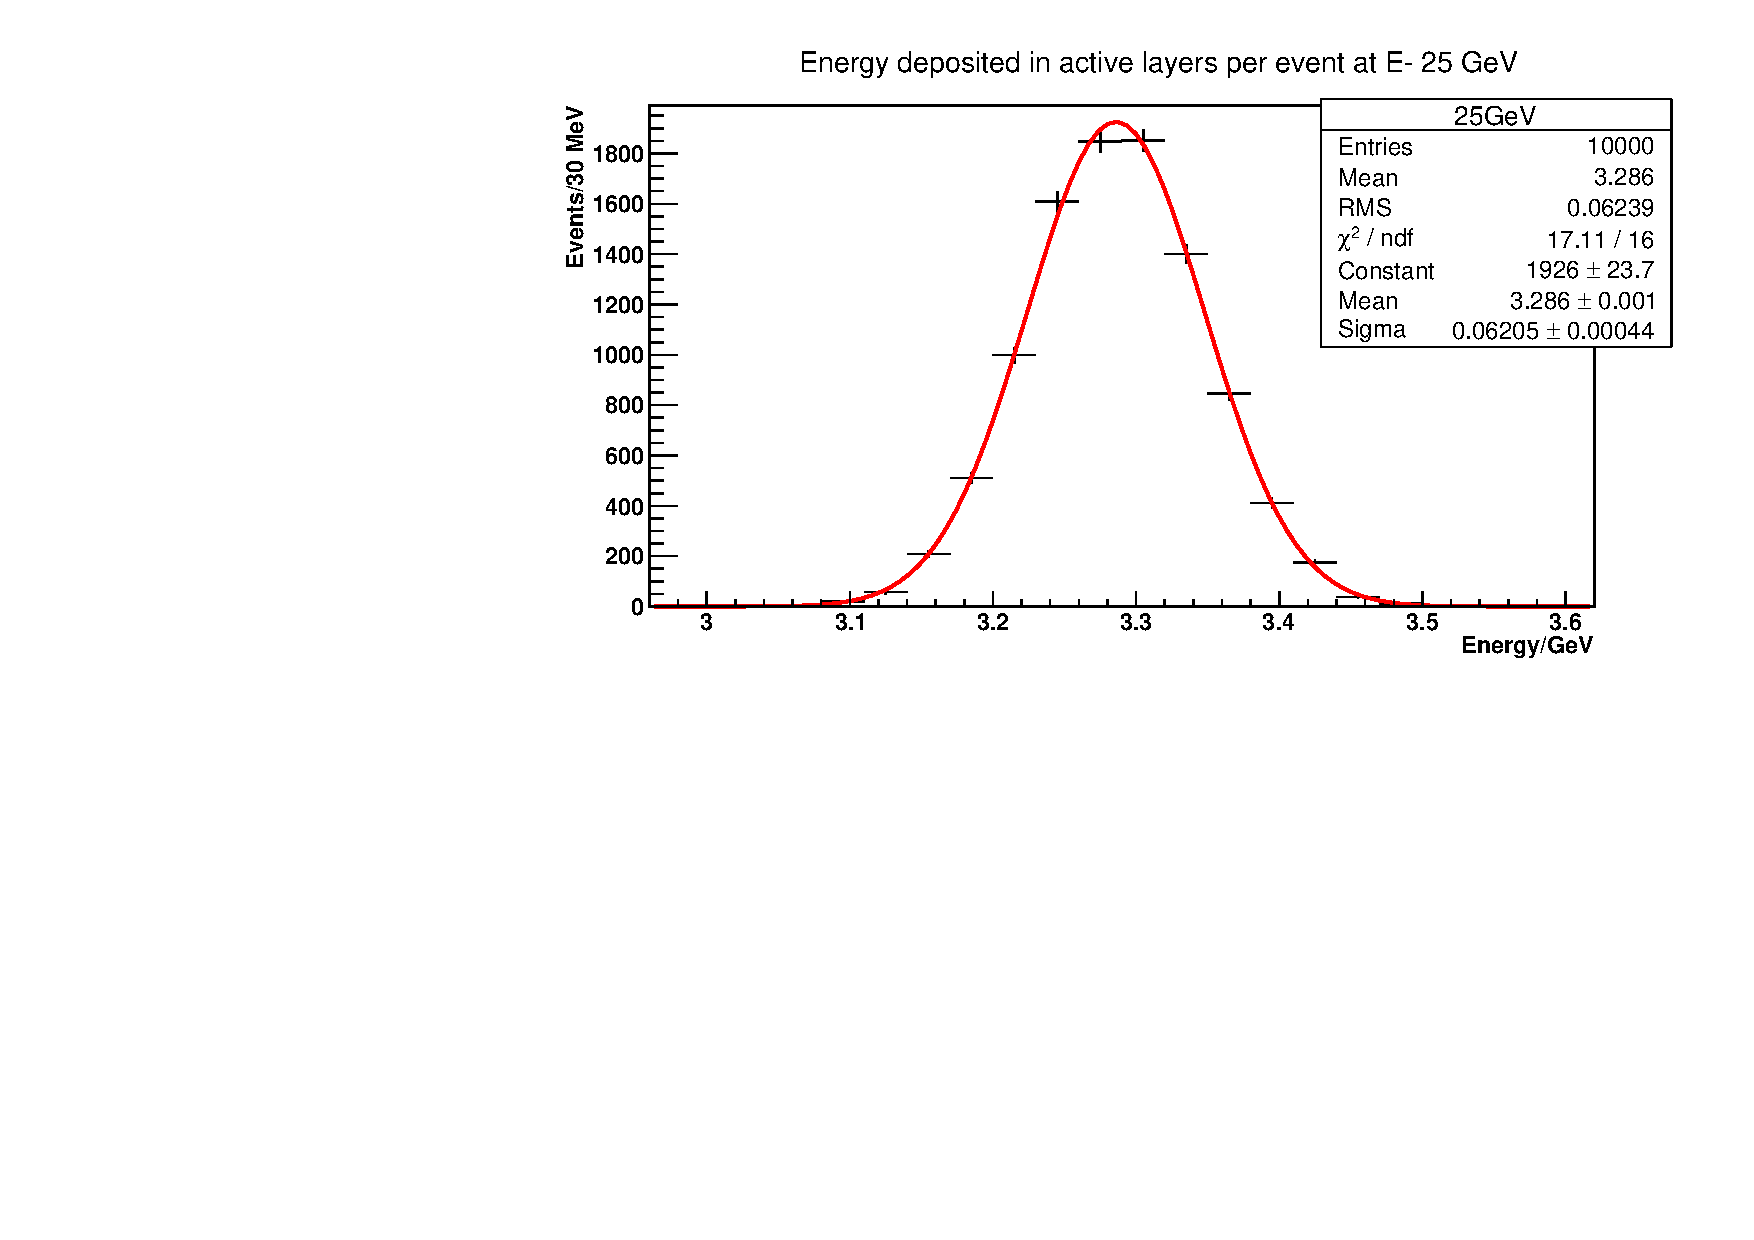
\includegraphics[width=\textwidth]{GaussExample.pdf}
  \caption{The distribution of energy deposited in scintillator(active) layers at 25 GeV}
  \label{fig:Gauss}
\end{figure}

From these fits the standard deviation divided by the mean was plotted against the incident particle energy, as defined in the configuration of \geant.  $\frac{\sigma}{E}$ is expected to follow equation \ref{eq:fr} but without the b term. Therefore a mimimum chi squared fit to,
\begin{equation}
  \label{eq:fitfr}
  \frac{\sigma}{E}=\frac{a}{\sqrt{E}}\bigoplus c
\end{equation}
was performed with the parameters 'a' and 'c' left floating.  This process was applied to both \geant version 9.5.p02 and 9.6.p04 with the same energies and 10000 events at each energy.  The results of these fits for both \geant versions are shown in figure \ref{fig:straightres} and table \ref{tab:results}.
\begin{figure}[h]
  \centering
  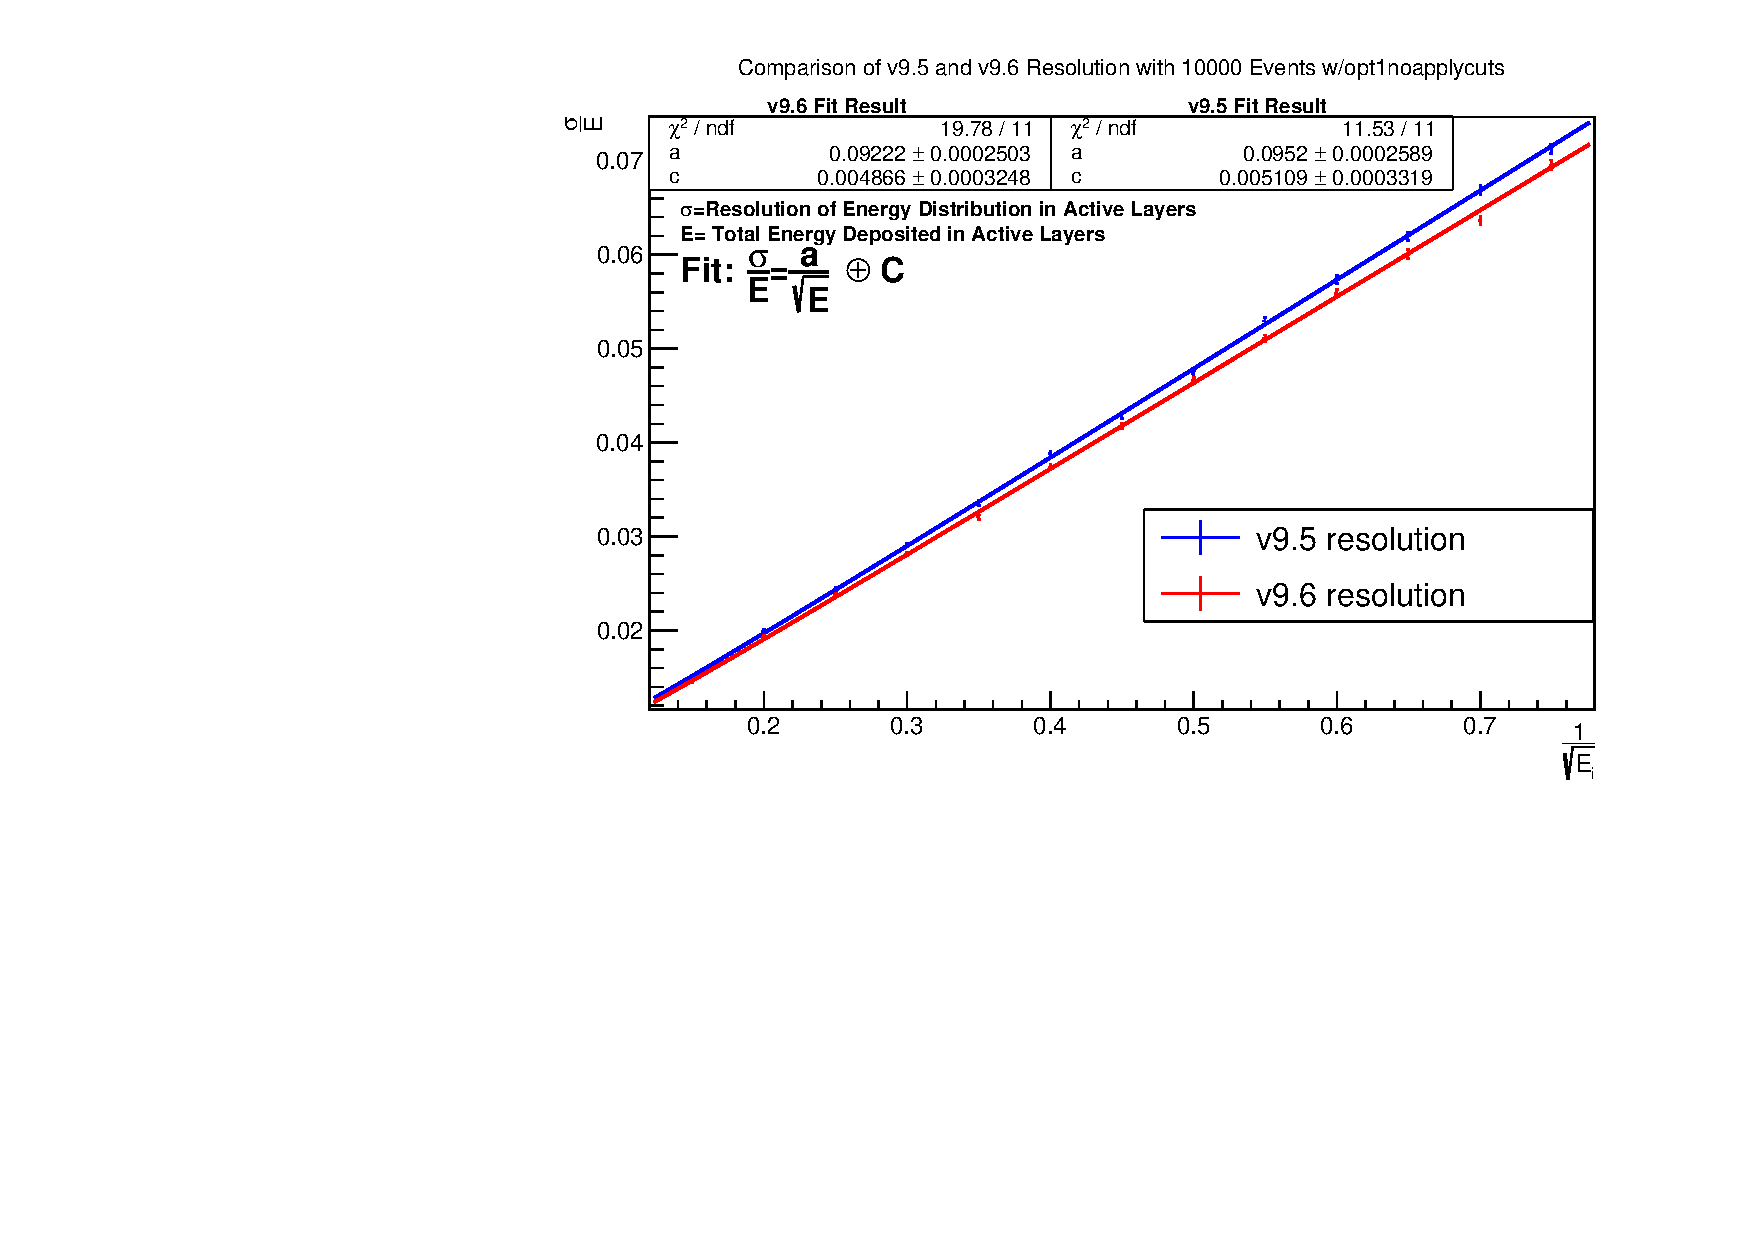
\includegraphics[width=\textwidth]{StraightCompareUse.pdf}
  \caption{A plot of fractional resolution against $\frac{1}{\sqrt{E}}$ comparing versions of \geant. The fit is the function given in equation \ref{eq:fitfr}.}
  \label{fig:straightres}
\end{figure}
%\begin{figure}[h]
 % \centering
  %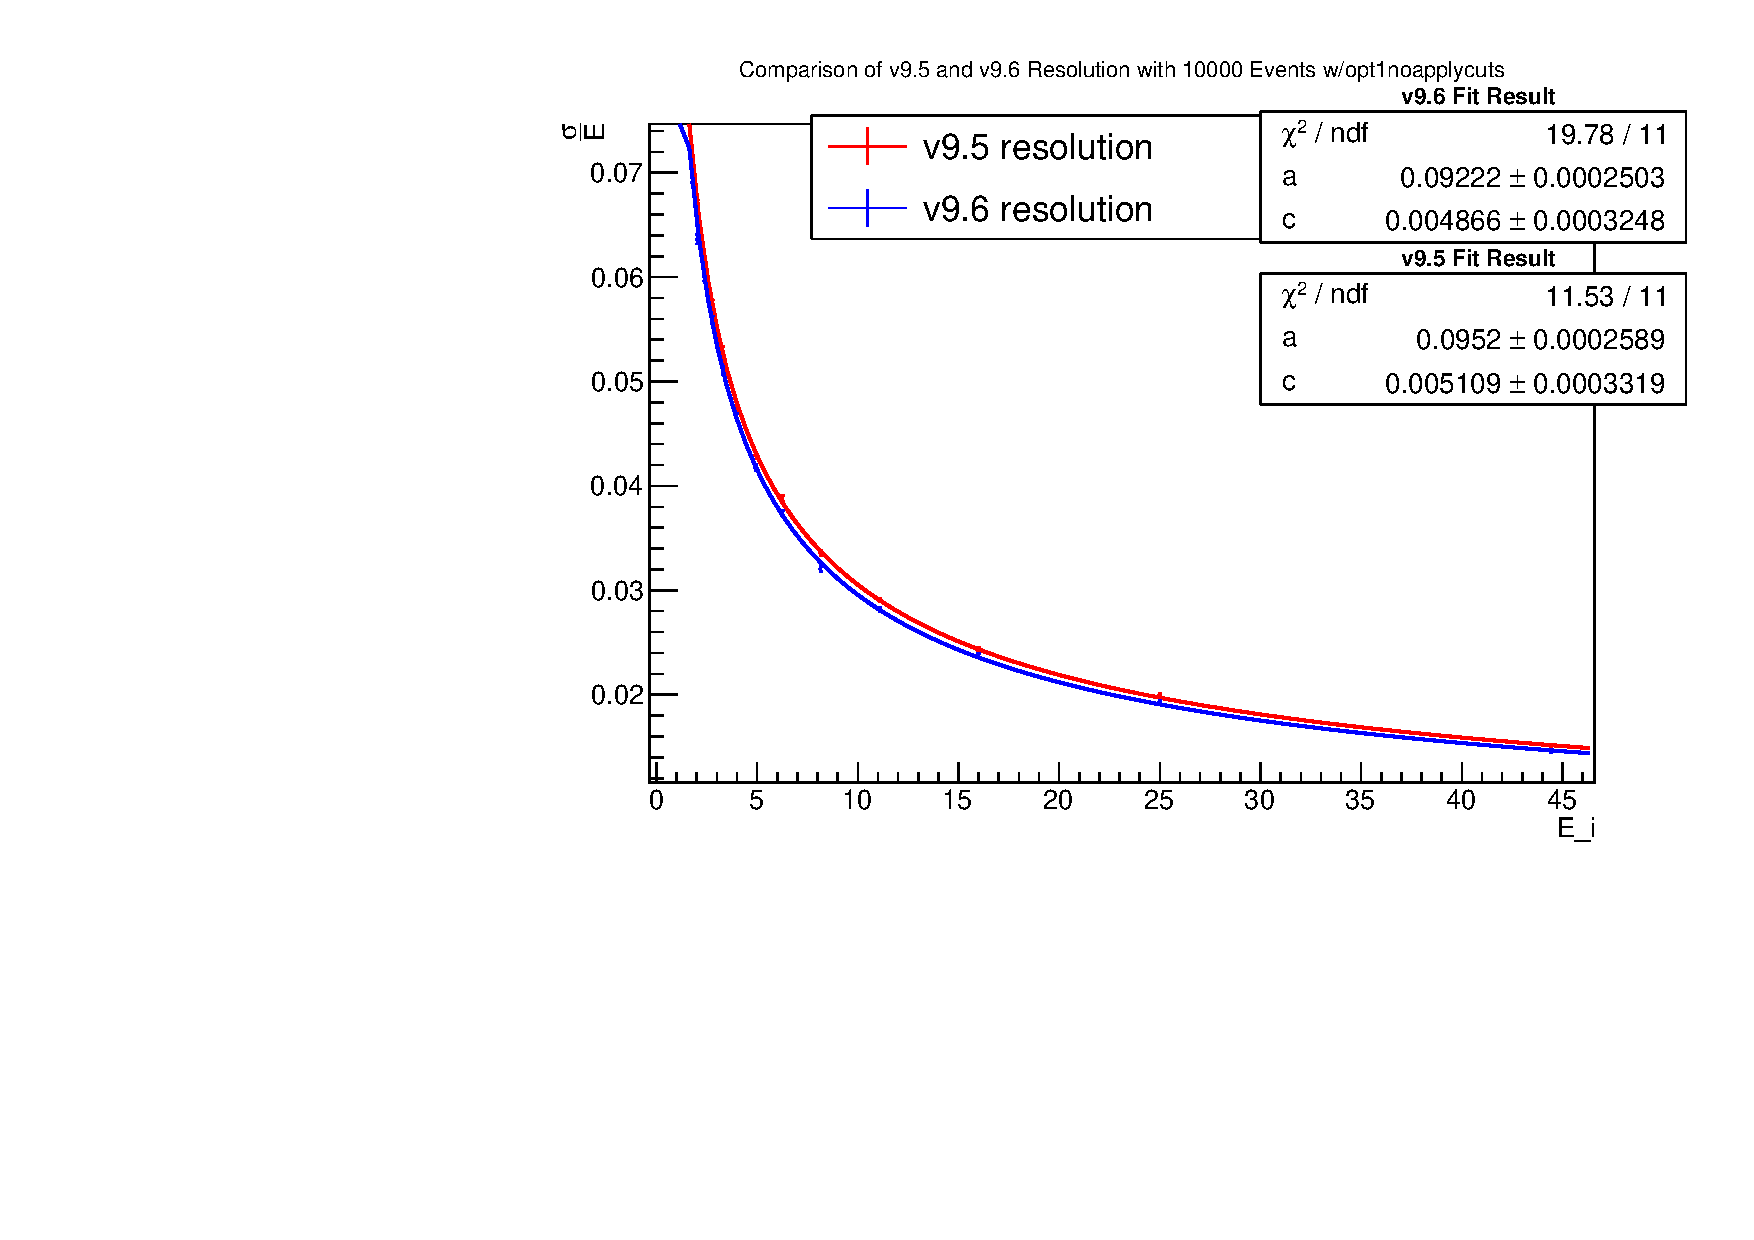
\includegraphics[width=\textwidth]{CurvedCompare.pdf}
  %\caption{A plot of fractional resolution against $E$ comparing versions of \geant. The fit is the function given in equation \ref{eq:fitfr}.}
  %\label{fig:coolres}
%\end{figure}

\begin{table}[h]
  \centering
  \begin{tabular}{|c|c|c|c|}
      \hline
      Version: & v9.5 & v9.6 & Difference  \\ \hline
      A term    & 0.0952$\pm$0.0003 & 0.0922$\pm$0.0003  & 8.43$\sigma$, 3.3\% \\ \hline
      C term    & 0.0051$\pm$0.0003 & 0.0049$\pm$0.0003 & consistent \\ \hline
      $\frac{\chi^2}{ndf}$   &1.798  & 1.048 &  \\ \hline
  \end{tabular}
  \caption{Fractional resolution results for comparison of \geant versions.  These results are obtained from the fits shown in figures \ref{fig:straightres}}
  \label{tab:results}
\end{table}

It is clear from these fits that there is a significant discrepancy in the statistical term of the fractional resolution parameterisation between \geant versions, despite the same PL being used in both versions.  The simulation of electromagnetic showers is a well established process that, in general, shows good agreement with data.  Therefore, progression of results this significant is not expected.  As many different processes contribute to electromagnetic showering more investigations were needed to understand exactly which part of the simulation is giving rise to this discrepancy.

\paragraph{Sampling Fraction and Shower Profile Investigations}
\label{sec:Sampling Fraction and Shower Profile Investigations}
In order to understand the unexpected results described in section \ref{sec:Fractional Resolution Investigation} it was decided that a study of the shower profiles in both active and passive layers of the calorimeter would be performed.  A shower profile is a plot of dE/dX against X, where X is the longitudinal depth from the front face of the calorimeter and E is the energy deposited.  Although X is often expressed in terms of radiation lengths, in this case the layer number was used because the shower profiles were in bins corresponding to the thickness of one layer of the ECAL.

Again, electrons at 13 different energies between 1.78GeV and 44.44GeV were fired into the ECAL using both \geant versions.  At each energy, shower profiles for active and passive layers were considered seperately and the profiles resulting from each version of \geant were plotted on top of each other for comparison.  The results at 1.78GeV and 44.44 GeV are shown in figures \ref{fig:1.78sp} and \ref{fig:44.44sp} respectively, all other energies are shown in \ref{ap:sp}.
\begin{figure}[h]
  \centering
  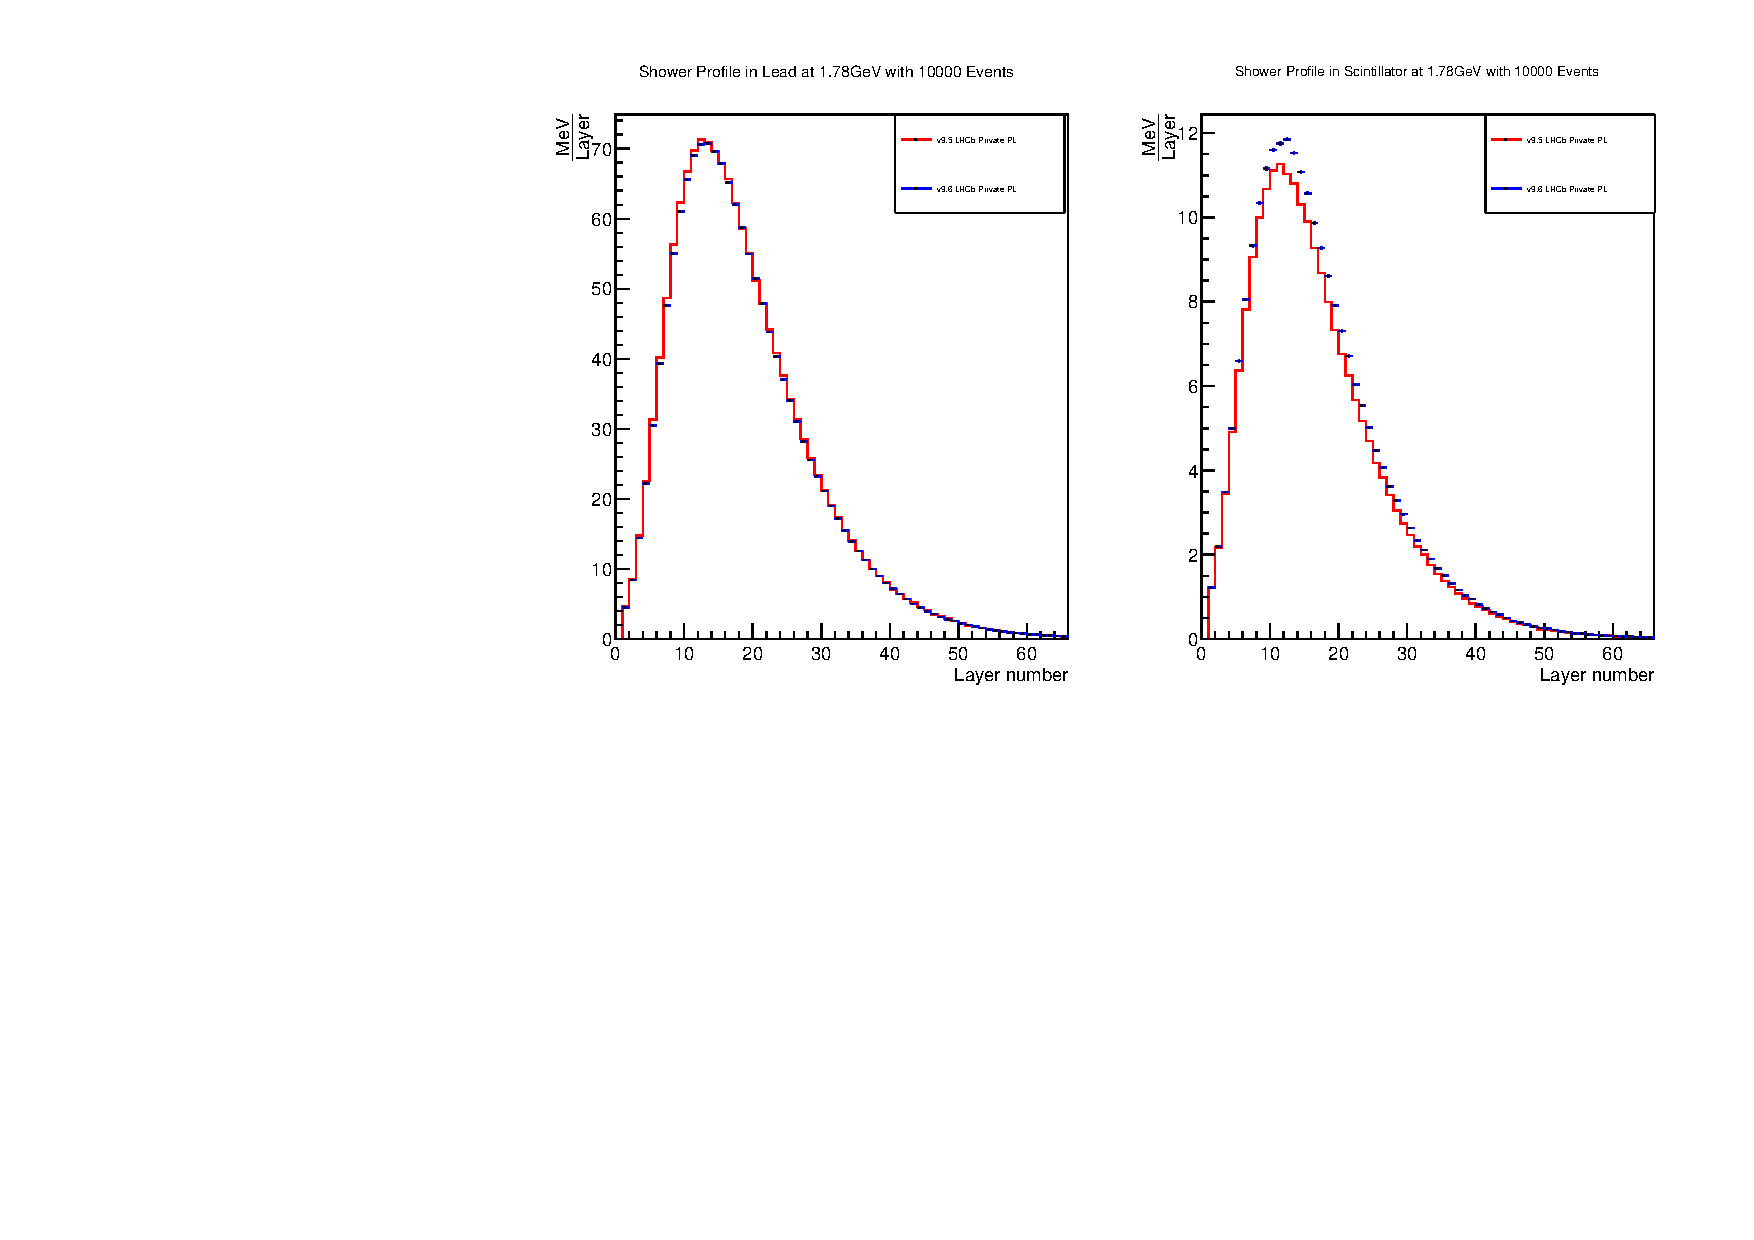
\includegraphics[width=\textwidth]{ShowerProfiles178.pdf}
  \caption{A comparison of shower profiles between \geant version 9.5 and 9.6 using the \lhcb private physics list for 1.78GeV electrons.  These profiles are normalised.}
    \label{fig:1.78sp}
\end{figure}
\begin{figure}[h]
  \centering
  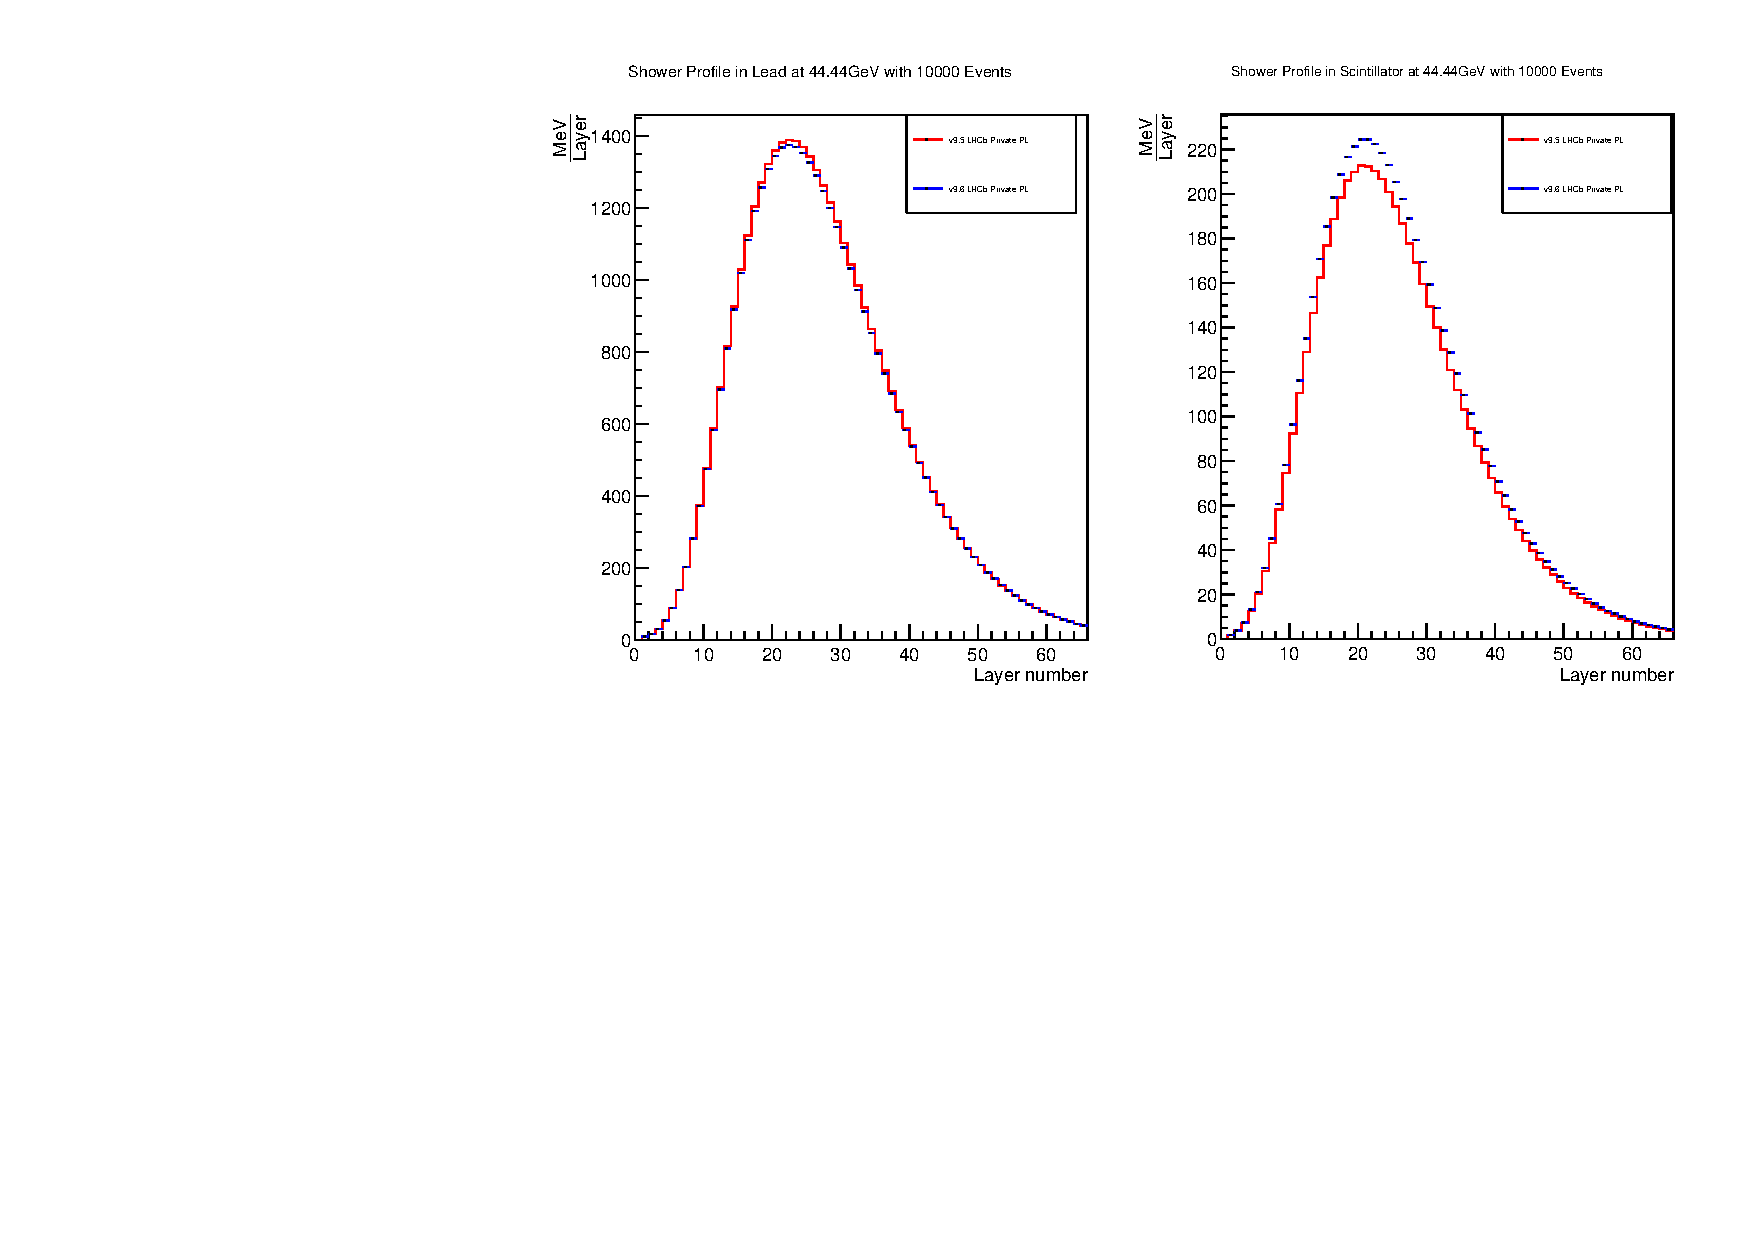
\includegraphics[width=\textwidth]{ShowerProfiles44.pdf}
  \caption{A comparison of shower profiles between \geant version 9.5 and 9.6 using the \lhcb private physics list at 44.44GeV electrons. These profiles are normalised.}
    \label{fig:44.44sp}
\end{figure}

It is clear from these shower profiles that \geant version 9.6.p04 is depositing more energy in active layers and less energy in passive layers compared to \geant 9.5.p02.  This pattern is observed at all energies simulated.

%To further investigate this behaviour the shower profiles were split by particle type; seperate shower profiles were plotted for electrons, positrons and photons.  These results can be seen in figures \ref{fig:1.78spseperate}  and \ref{fig:44.44spseperate}.
%PUT SEPERATE SHOWER PROFILES HERE
%These reuslts show that the observed discrepancy can not be attributed to the way in which photons are modelled because the total energy deposited by photons is negligable and would therefore not be able to influence the overall shower profiles.

In order to quantify further this observed change in behaviour, the ECAL sampling fraction as a function of energy was studied for both \geant versions.  The sampling fraction, in this context, is defined as the energy deposited in active layers (visible energy) divided by the incident particle energy.  The total energy deposited in each type of material was obtained by integrating the shower profiles over all layers.  The resulting sampling fraction as a function of energy is shown in \ref{fig:sfcomp}.
\begin{figure}[h]
  \centering
  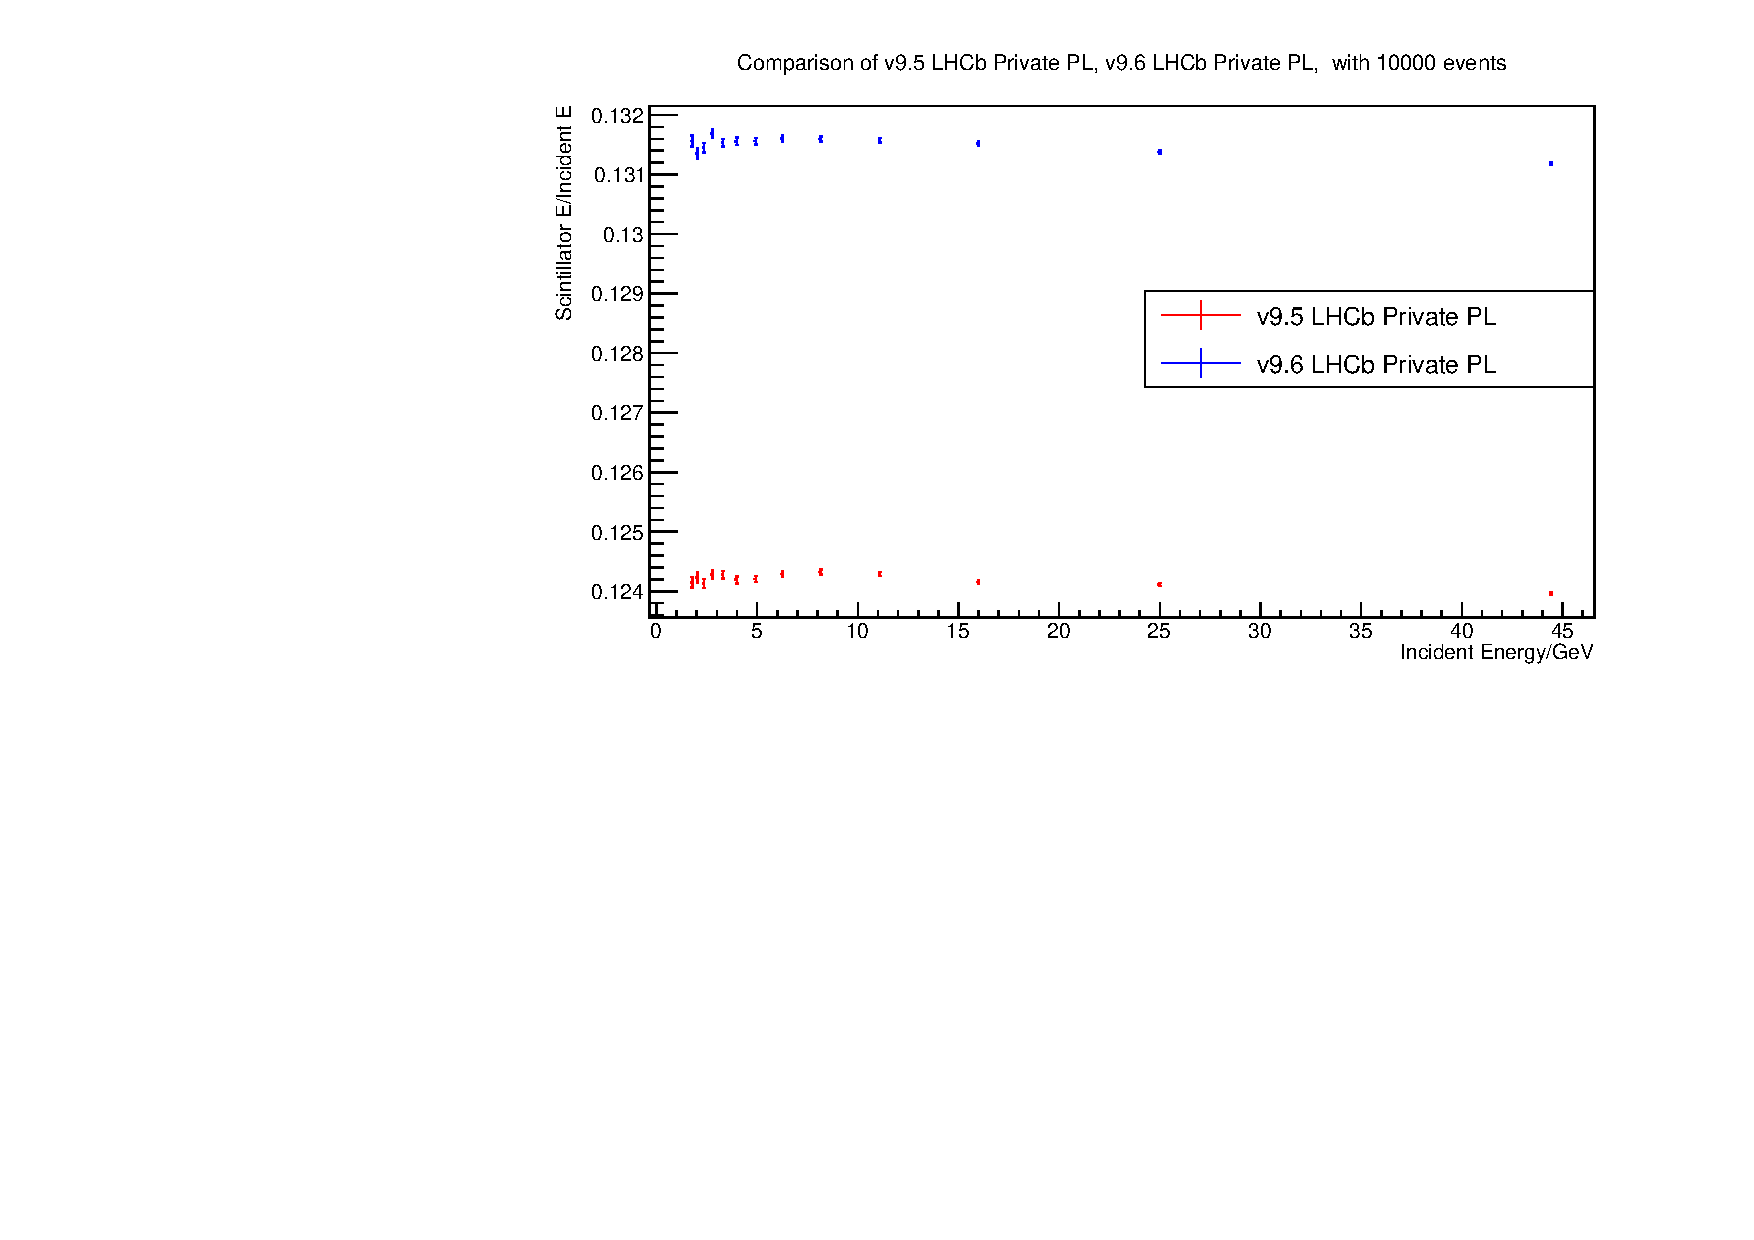
\includegraphics[width=\textwidth]{SamplingFractionVersions.pdf}
  \caption{A plot of sampling fraction as a function of energy for both versions of \geant}
  \label{fig:sfcomp}
\end{figure}
To further this quantification the ratio of energy deposited in active layers to passive layers was also plotted as a function of energy for both \geant versions and the results are shown in figure \ref{fig:ratiocomp}.
\begin{figure}[h]
  \centering
  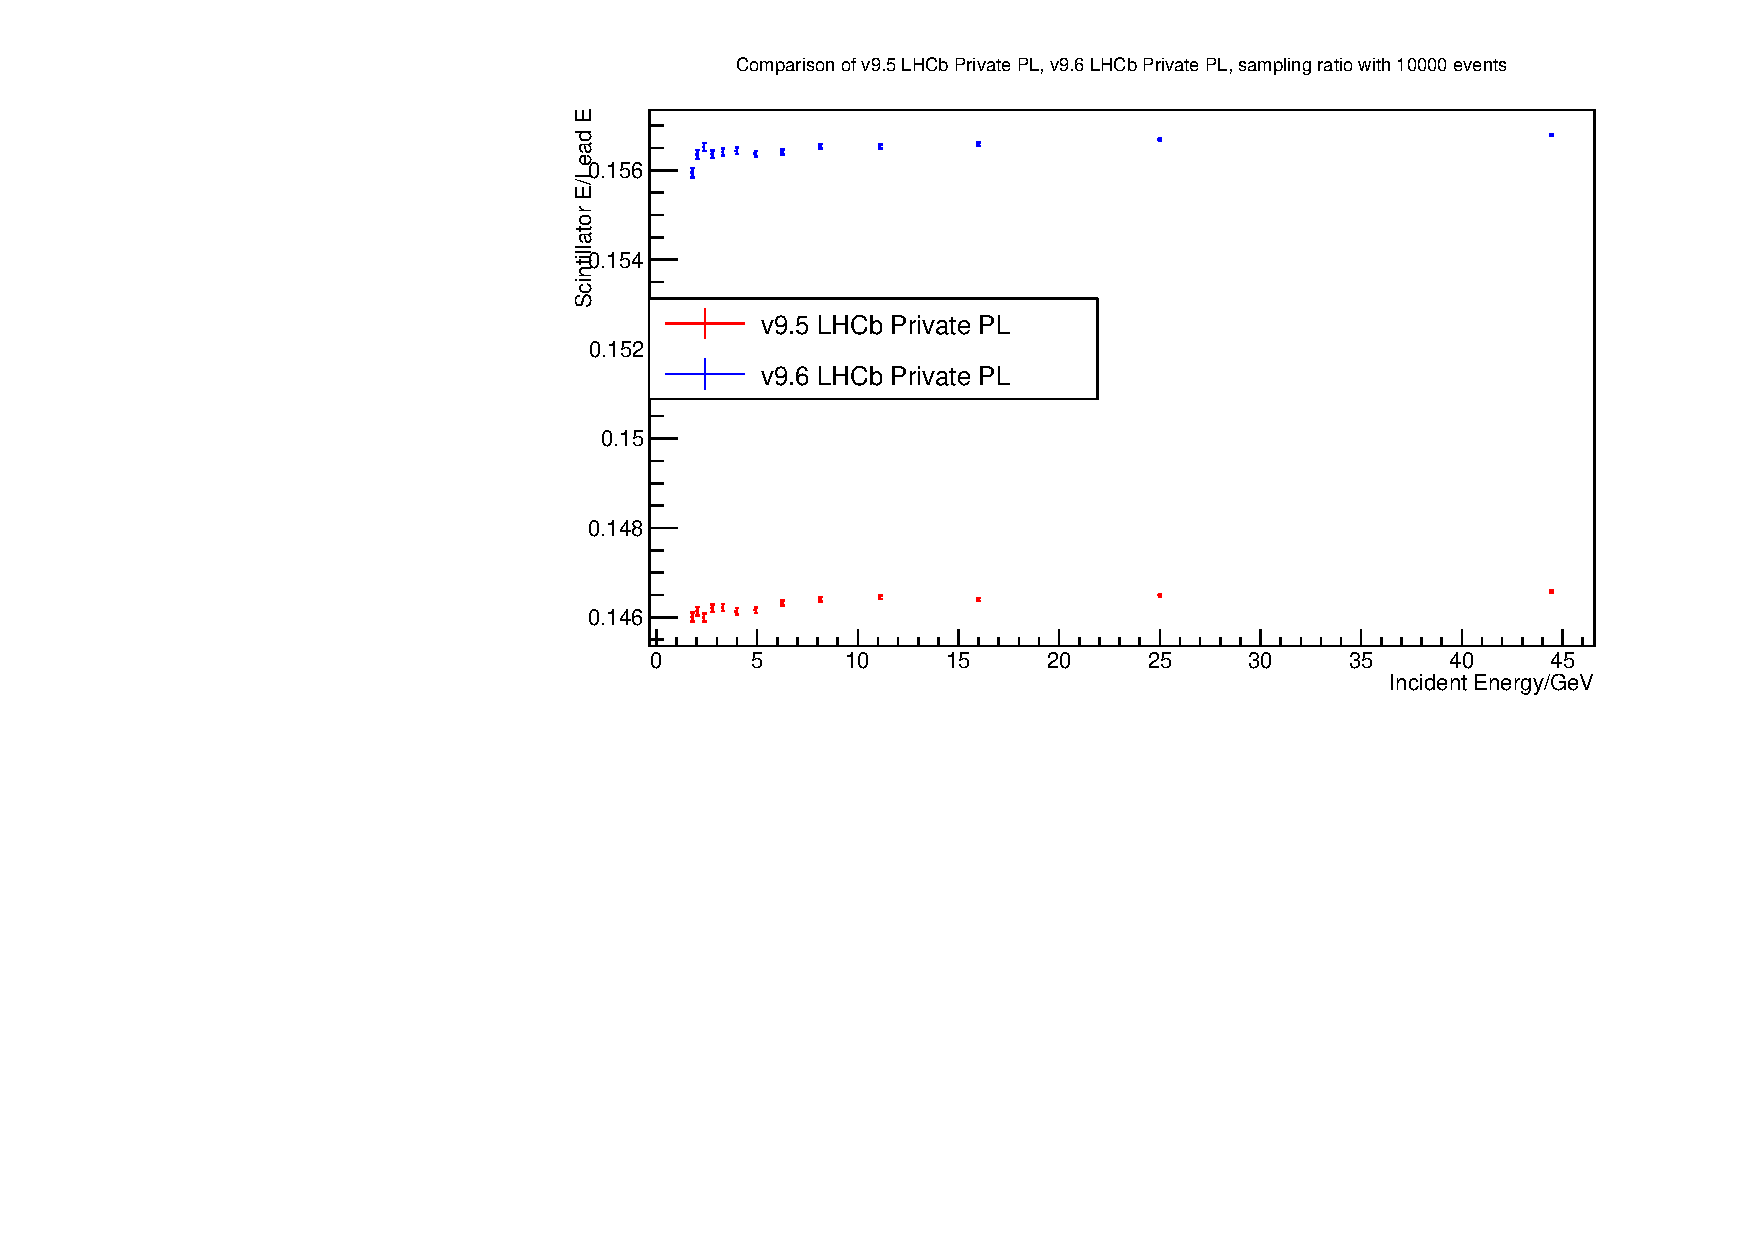
\includegraphics[width=\textwidth]{SamplingRatioVersions.pdf}
  \caption{A plot of the ratio of energy deposited in active layers to passive layers as a function of energy for both \geant versions}
  \label{fig:ratiocomp}
\end{figure}
The results from the investigation of sampling fraction and sampling ratio are summarised in table \ref{tab:sfcomp}.

\paragraph{Discussion of results for \geant version comparison}
\label{sec:Discussionofresultsone}
The results of these sampling fraction studies are significant, both statistically and in terms of the implications for the next simulation package used by \lhcb.  It is very clear that the sampling fractions have changed between \geant versions and this change would explain the observed discrepancy in fractional resolution seen in section \ref{sec:Fractional Resolution Investigation}.  Sampling more energy would always improve the fractional resolution of an ECAL because it means any statistical fluctutations are relatively less significant. The ECAL has to be calibrated in monte carlo such that an observed value of visible energy corresponds to the correct incident energy.  Since these results show that the visible energy of the ECAL has changed in this new version of \geant this calibration will have to be performed again when the new simulation package is released.

The precise cause of these discrepancies needs to be understood because there could be implications for the simulation of other detector components.

After contacting the \geant collaboration, the cause of the observed discrepancy is believed to lie with the changes to the multiple scattering model.  In fact, the \geant collaboration recommended that the multiple scattering models used in the \lhcb private PL are changed from \textit{UrbanMsc95} to \textit{UrbanMsc93} below 100MeV and \textit{WentzelVI} above 100MeV.  This would bring the simulation of multiple scattering within the LHCb private PL inline with the \geant \textit{emstandard opt1} physics list.
\clearpage
\subsubsection{Comparison of Physics Lists}
\label{sec:Comaprison of PL}
As the \geant collaboration had recommended a change to the LHCb private PL it was decided a thorough investigation of other PL options would be carried out using the simple calorimeter test.  This would be done using \geant version 9.6.p04, so that investigations directly related to the next version of the \lhcb simulation package could be carried out.  The results of these investigations would help to inform the decision of which PL to use for the next release of \gauss.  

The following physics lists supplied by \geant were investigated:
\begin{itemize}
\item \textit{emstandard option0}
  This is the default electromagnetic phyics list used by \geant (in general).  This is designed to give optimal accuracy at medium and high energies, which are the typical energies present at HEP experiments.  In version 9.6 this PL uses the \textit{UrbanMsc95} multiple scattering model.
\item \textit{emstandard option1}
  This physics list is designed for HEP experiments but is described as \cms focused. This PL has moved back to using the \textit{UrbanMsc93} multiple scattering model below 100MeV and the WentzelVI model above 100MeV in version 9.6.  It also uses the \textit{minimal} step limit type which applys looser limitations on the maximum length of a single simulation step.  This results in less steps being simulated, leading to large savings in CPU time.  However, this is known to cause bias in the results and this bias increases for longer production cuts \cite{1742-6596-219-3-032045}.
\item \textit{emstandard option2}
  This physics list is also designed for HEP experiements but is described as \lhcb focused.  It uses the \textit{UrbanMsc93} multiple scattering model and uses a different angular distribution generator for bremsstrahlung.  Like \textit{opt1} it also uses the \textit{minimal} step limit type to save CPU time at the expense of accuracy.
\item \textit{emstandard option3}
  This PL provides the best accuracy of charged particle tracking in the absence of a magnetic field.  It uses the \textit{UrbanMscModel96} for multiple scattering.
\item \textit{emstandard option 4}
  This PL, like option 3, is designed to provide the best accuracy for charged particle tracking in the absence of a magnetic field and also uses the \textit{UrbanMscModel96} for multiple scattering.  However, it is designed to provide the highest accuracy at medium and low energies.
\end{itemize}

As well as the \geant supplied PLs there is also the \lhcb private physics list to consider.  This is simply \textit{emstandard option1} with the \textit{applycuts} option disabled.  However, it is based on the \textit{opt1} PL from \geant v9.4 which differs to both the v9.5 and v9.6 \textit{opt1} PLs.  Therefore, rather than just updating the multiple scattering model used in the \lhcb private PL (as suggested by the \geant collaboration  and discussed in section \ref{sec:Discussionofresultsone}) it was decided that the new version of the \lhcb private PL would be the \textit{opt1} PL from v9.6 with the \textit{ApplyCuts} option disabled. Consequently, this study investigates both the old version of the \lhcb private PL (LHCbOld) and the new version (LHCbNew).

\paragraph{Fractional Resolution}
The first quantity used to test all the PLs described above was, again, the fractional resolution of the model ECAL.  Just as described in section \ref{sec:Fractional Resolution Investigation}, 10000 electrons were fired into the model ECAL at 13 different energies between 1.78GeV and 44.44GeV.  The same procedure as described in section \ref{sec:Fractional Resolution} was again used to extract $\frac{\sigma}{E}$ for each energy and a minimum $\chi^2$ fit to equation \ref{eq:fitfr} was performed to obtain the values of 'a' and 'c'.  The simulation was run with all of the PLs described in section \ref{sec:Comparison of PL}, allowing them to all be considered as a potential PL for the next version of \gauss.
\begin{figure}[h]
  \centering
  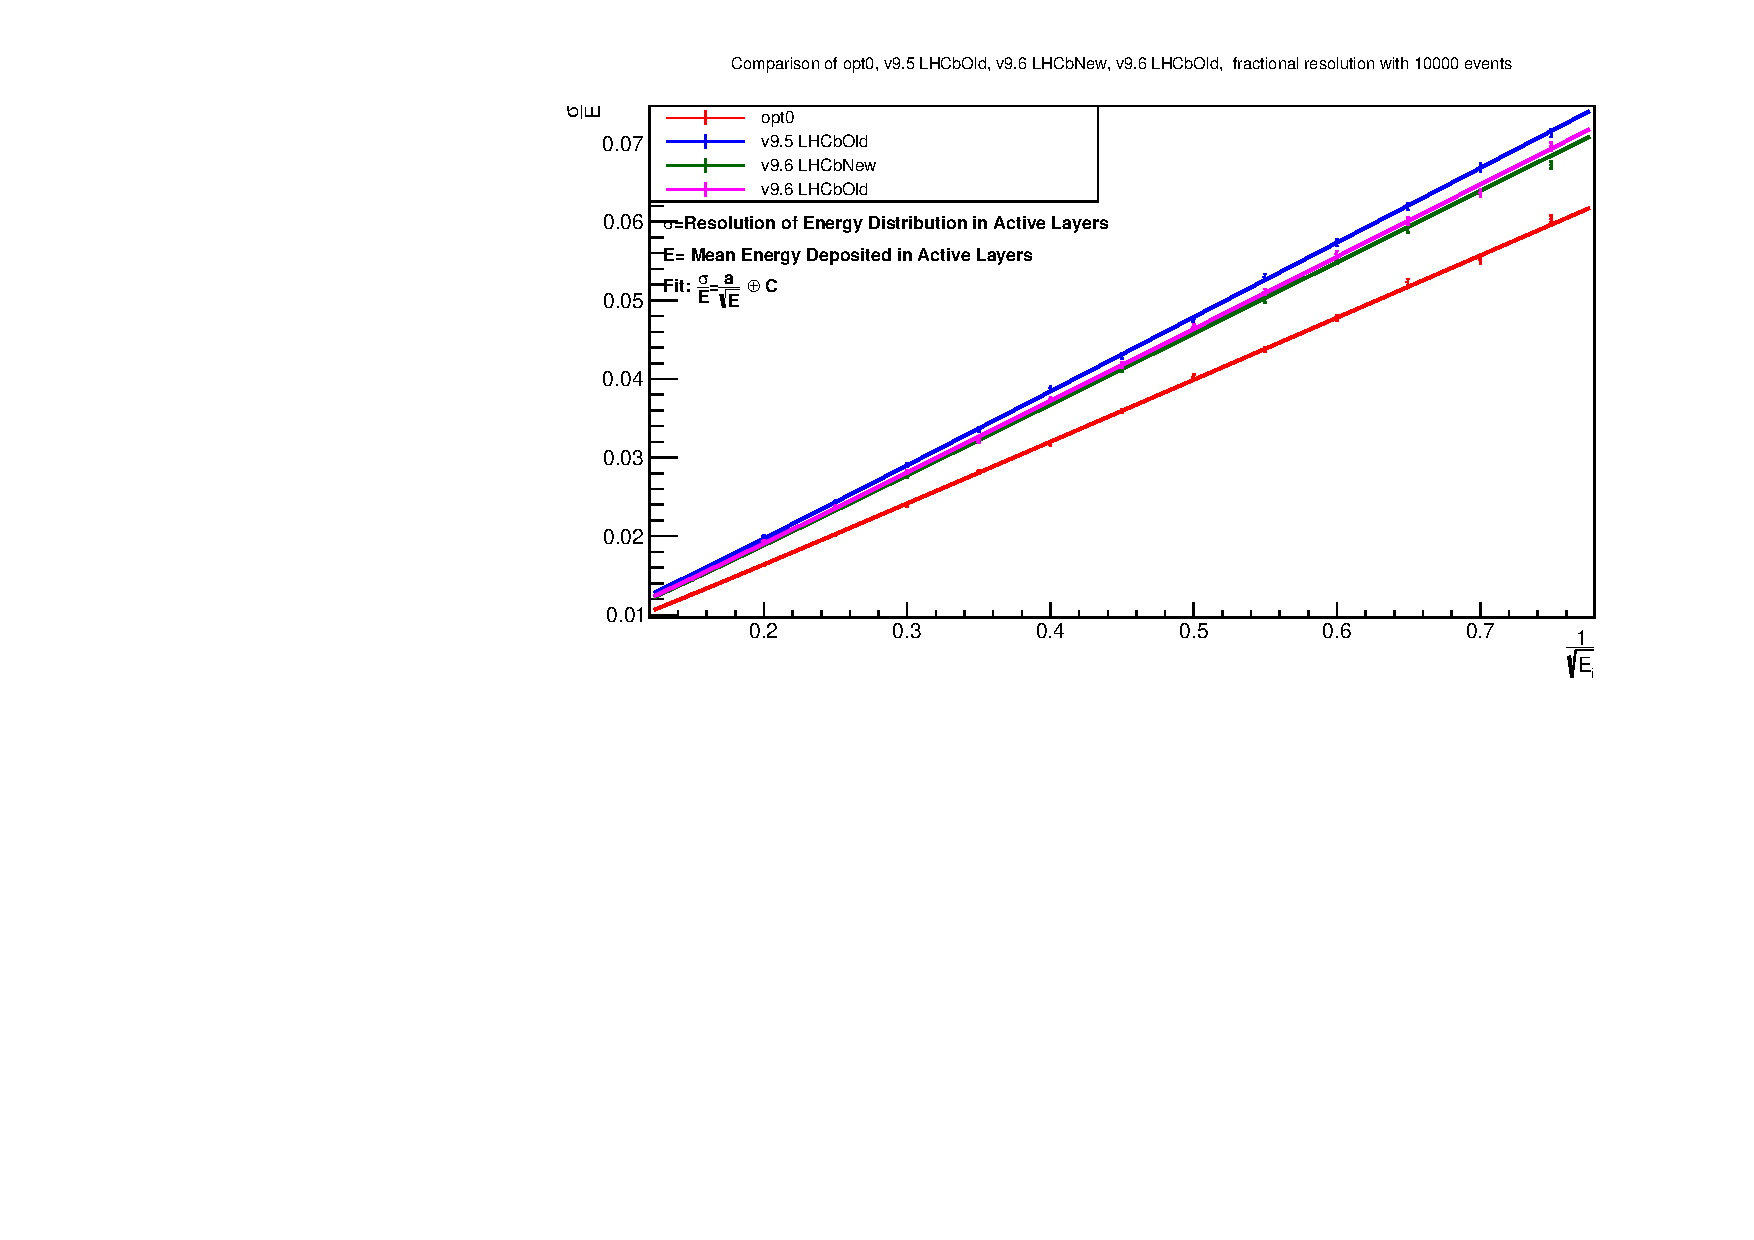
\includegraphics[width=\textwidth]{LHCbPLsStraight2.pdf}
  \caption{A plot of fractional resolution against $\frac{1}{\sqrt{E}}$ for \geant v9.5 with the old PL and v9.6 with the new and old physics list options}
  \label{fig:LHCbPLStraightFR}
\end{figure}

Figure \ref{fig:LHCbPLStraightFR} shows the fractional resolution results with the two LHCb private PL options, the results from v9.5 and the opt0 physics lists are included for comparison. A similar comparison is also made between all of the standard PLs supplied by the \geant collaboration, which is shown in Figure \ref{fig:BoxPLStraightFR}.  A summary of all fit results is shown in Table \ref{tab:AllPL}
\begin{figure}[h]
  \centering
  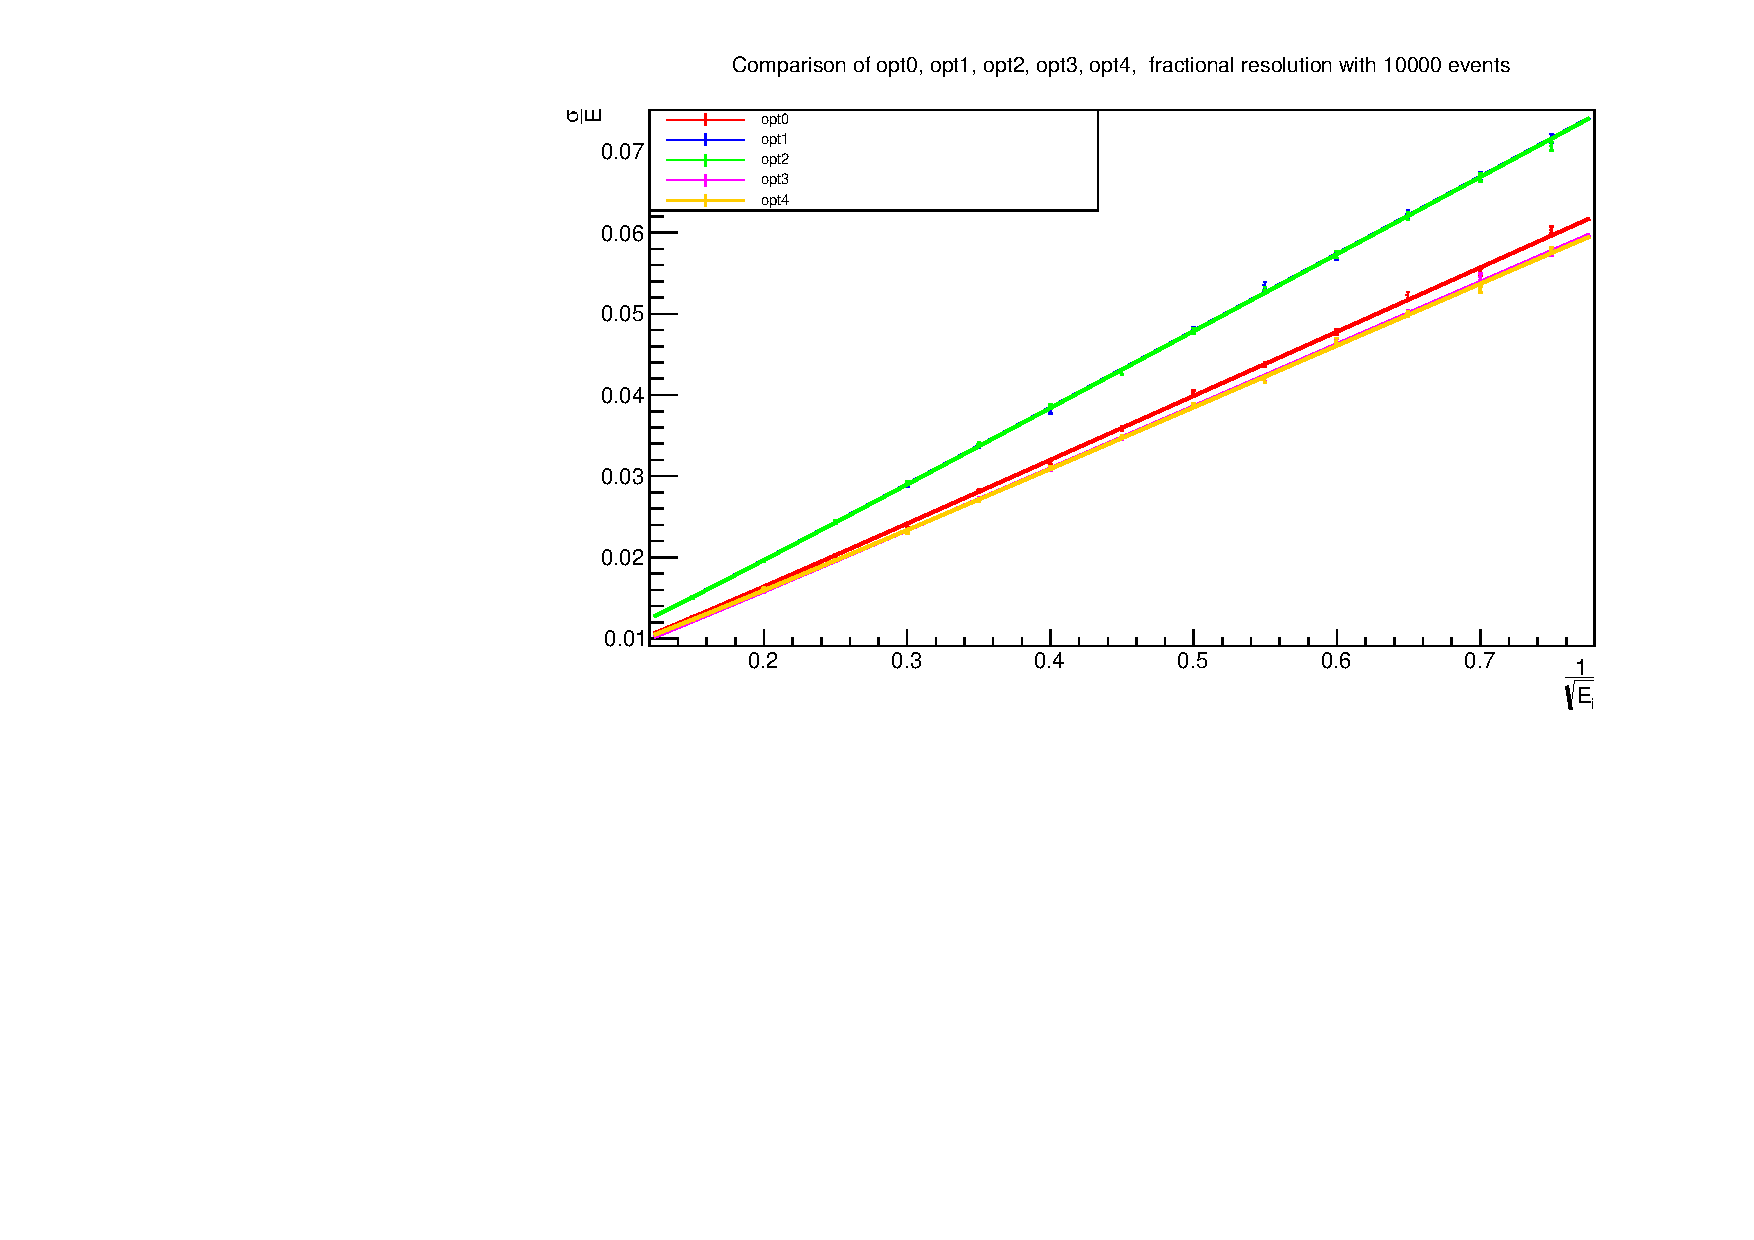
\includegraphics[width=\textwidth]{BoxStraightRes.pdf}
  \caption{A plot of fractional resolution against $\frac{1}{\sqrt{E}}$ for \geant v9.6 with all of the \textit{emstandard} PLs.}
  \label{fig:BoxPLStraightFR}
\end{figure}

\begin{table}[h]
  \centering
  \begin{tabular}{|c|c|c|c|}
      \hline
      PL & A term & C term & $\frac{\chi^2}{ndf}$  \\ \hline
      v9.5 LHCbOld & 0.0952 $\pm$ 0.0003 & 0.0051 $\pm$ 0.0003 & 1.05 \\ \hline
      LHCbOld & 0.0922 $\pm$ 0.0003 & 0.0049 $\pm$ 0.0003 & 1.80 \\ \hline 
      LHCbNew & 0.0910 $\pm$ 0.0002 & 0.0049 $\pm$ 0.0003 & 1.55 \\ \hline
      opt0 & 0.0794 $\pm$ 0.0002 & 0.0041 $\pm$ 0.0003 & 1.39 \\ \hline
      opt1 & 0.0953 $\pm$ 0.0003 & 0.0048 $\pm$ 0.0004 & 0.91 \\ \hline
      opt2 & 0.0953 $\pm$ 0.0003 & 0.0048 $\pm$ 0.0003 & 0.64 \\ \hline 
      opt3 & 0.0768 $\pm$ 0.0002 & 0.0037 $\pm$ 0.0003 & 0.67 \\ \hline 
      opt4 & 0.0764 $\pm$ 0.0002 & 0.0045 $\pm$ 0.0002 & 1.60 \\ \hline
  \end{tabular}
  \caption{Fractional resolution results for comparison of \geant physics lists.  These results are obtained from the fits shown in figures \ref{fig:LHCbPLStraightFR} and \ref{fig:BoxPLStraightFR}}
  \label{tab:AllPL}
\end{table}

Figure \ref{fig:LHCbPLStraightFR} shows that updating the \lhcb private PL to follow \textit{emstandard opt1} has, in fact, increased the discrepancy with v9.5.  Although this initially seems troublesome, one should not necessarily expect the results from the new PL to match those of the old PL and \geant version because progression of results is expcected.  There is nothing to say the old PL would show the best agreement with data, in fact one should expect the newer version to be the most accurate.  It is, however, important that the progression of results is observed and calibrated for.

A direct comparison with data is not possible in this scenario due to limited test beam data and the absence of electronic noise in this simplifed scenario.   It is known that the \lhcb private PL has to use a simplified and consequently bias multiple scattering model due to CPU time constraints.  Therefore, the PLs that do not use a simplifed multiple scattering model (namely \textit{opt0}, \textit{opt3} and \textit{opt4}) should provide the best agreement with data and can consequently be used to check if progress towards greater accuracy has been made.  On this basis, Figure \ref{fig:LHCbPLStraightFR} shows that progress towards a more accurate fractional resolution result has been made by both moving to \geant v9.6 and updating the \lhcb private PL. Nevertheless, progress this large for well understood electromagnetic processes is still surprising.

Figure \ref{fig:BoxPLStraightFR} shows that there is a big difference in results between models that use a simplifed multiple scattering model and those that don't.  There is almost no difference between \textit{opt1} and \textit{opt2}, both of which \textbf{do} use a simplified multiple scattering model.  Likewise, \textit{opt3}, \textit{opt4}, and \textit{opt0} show results that are within $5\%$ of each other, all of which \textbf{do not} use a simpified multiple scattering model.  This is useful confirmation that, as expected and observed by \geant themselves, simplifying the multiple scattering model with the \textit{minimal} step limit option introduces bias to the result \cite{1742-6596-219-3-032045}.

\paragraph{Sampling Fractions and Shower Profiles} 
Using the same procedure as descirbed in section \ref{sec:Sampling Fraction and Shower Profile Investigations} shower profiles were created for all PLs under investigation.  
\begin{figure}[h]
  \centering
  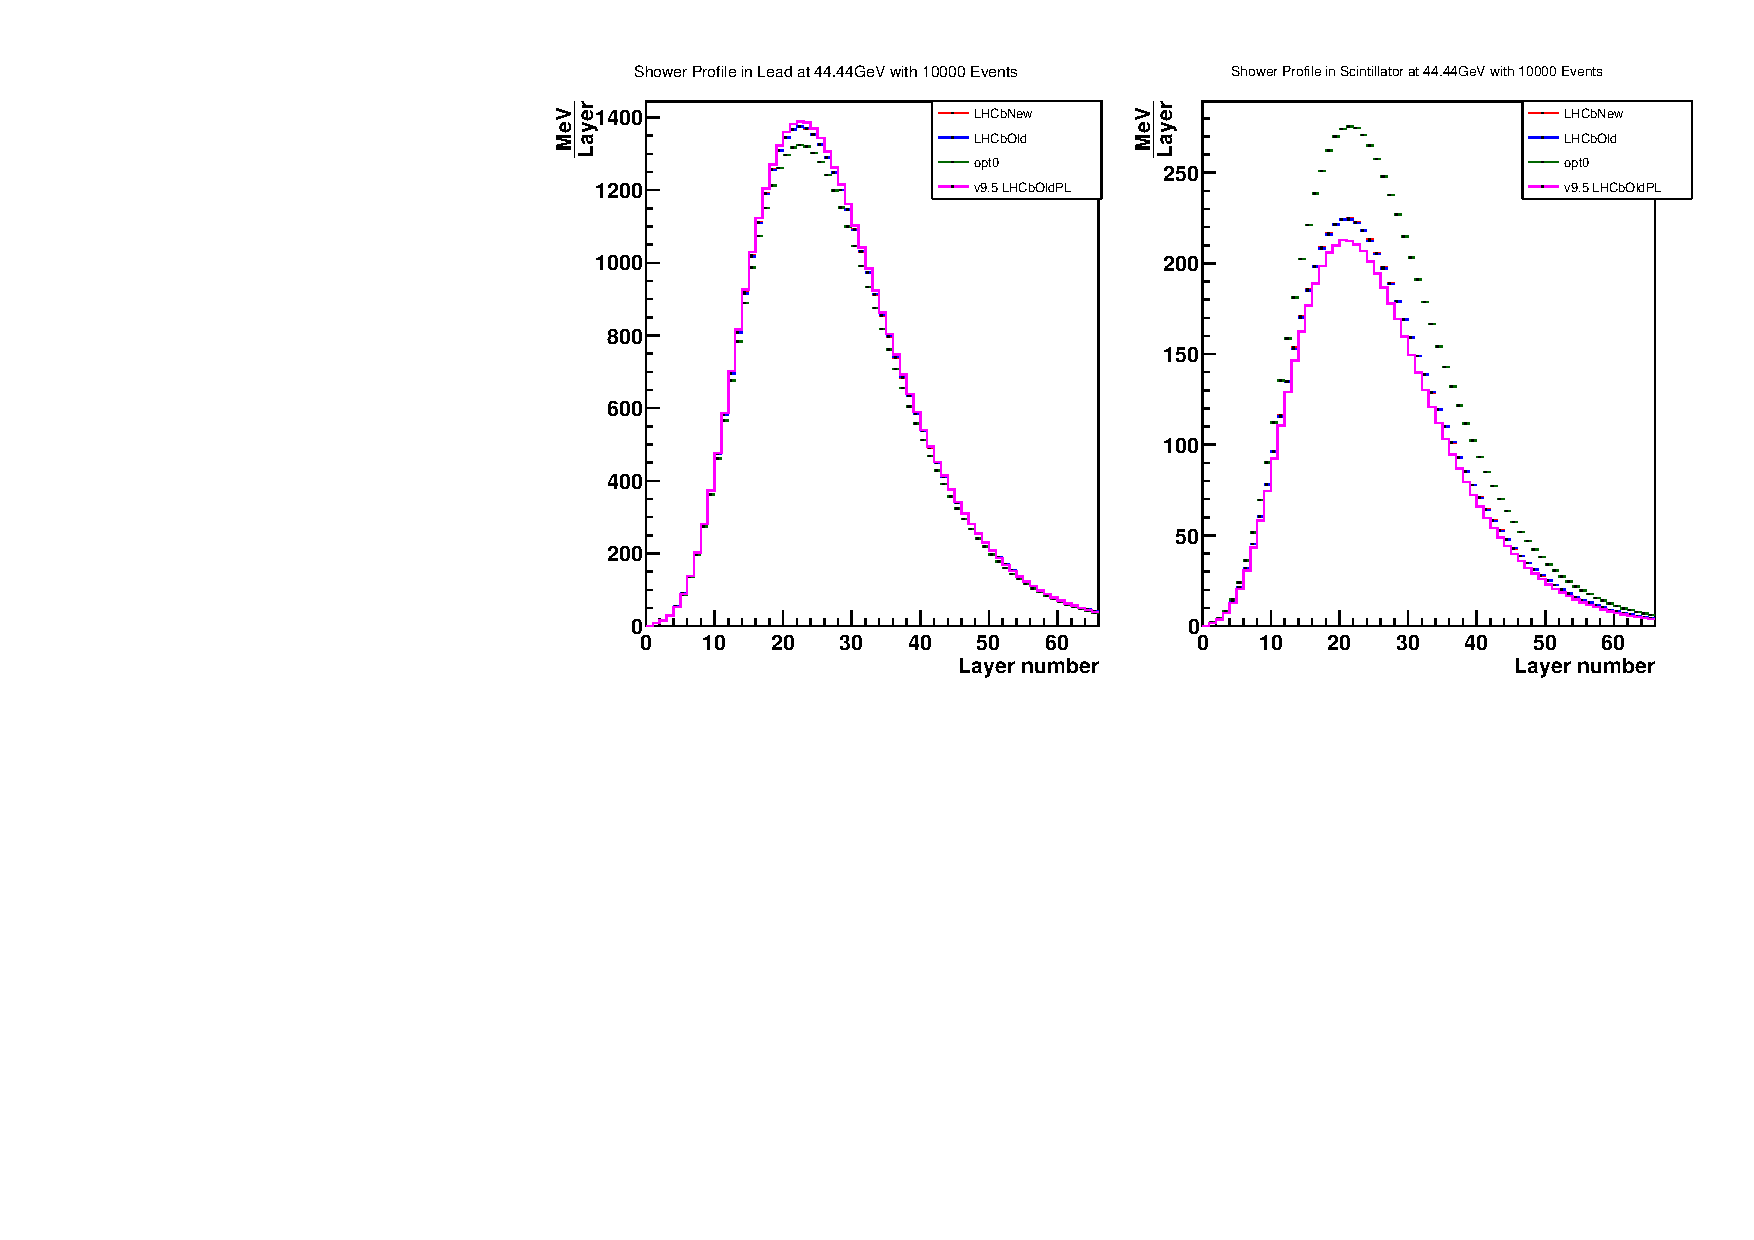
\includegraphics[width=\textwidth]{ProgressShowers.pdf}
  \caption{Shower profiles in Lead and Scintillator layers of the ECAL using LHCb private PLs and \geant PLs without simplified multiple scattering models.}
  \label{fig:LHCbPLShowers}
\end{figure}

Figure \ref{fig:LHCbPLShowers} shows shower profiles in lead and scintillator layers at 44.44GeV for the \lhcb private PLs; \textit{opt0} and the v9.5 results are included for comparison.  This shows that changing to \geant v9.6 has moved the shower profiles towards, what is understood to be, the results with the most accurate PL.  However, in the case of shower profiles the results from the new and old \lhcb private PLs are too close to draw any conclusions about which is the more accurate.

\begin{figure}[h]
  \centering
  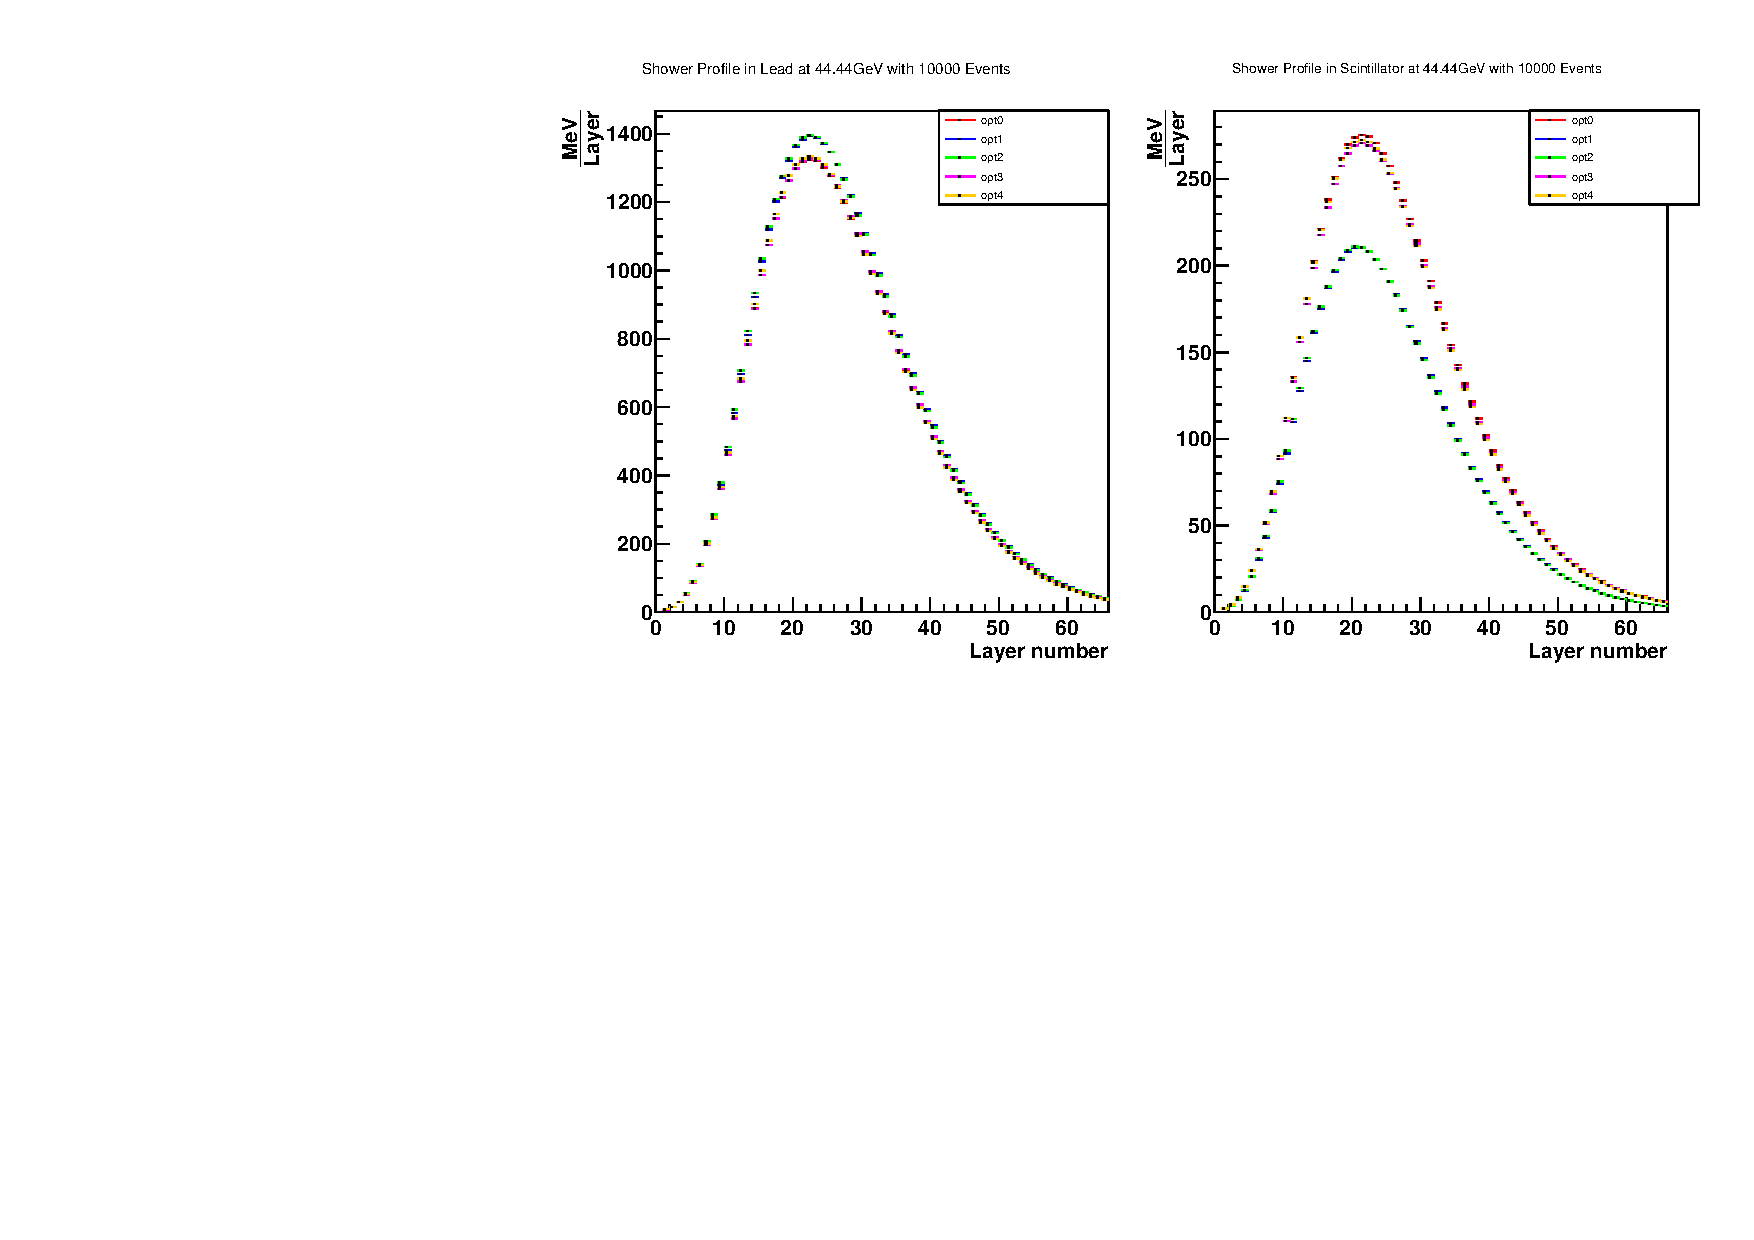
\includegraphics[width=\textwidth]{BoxShowers.pdf}
  \caption{Shower profiles in Lead and Scintillator layers of the ECAL using \geant supplied PLs}
  \label{fig:BoxPLShowers}
\end{figure}

Figure \ref{fig:BoxPLShowers} shows a comparison of shower profiles, in both mediums, for all of the \textit{emstandard} PLs.  This shows a significant discrepancy between PLs with and without a simplified multiple scattering model.  This is again useful confirmation that a simplified multiple scattering model does unfortuantely introduce bias to the results.


As in section \ref{sec:Sampling Fraction and Shower Profile Investigations} the shower profiles were integrated to obtain the sampling fraction and sampling ratio for each PL.
\begin{figure}[h]
  \centering
  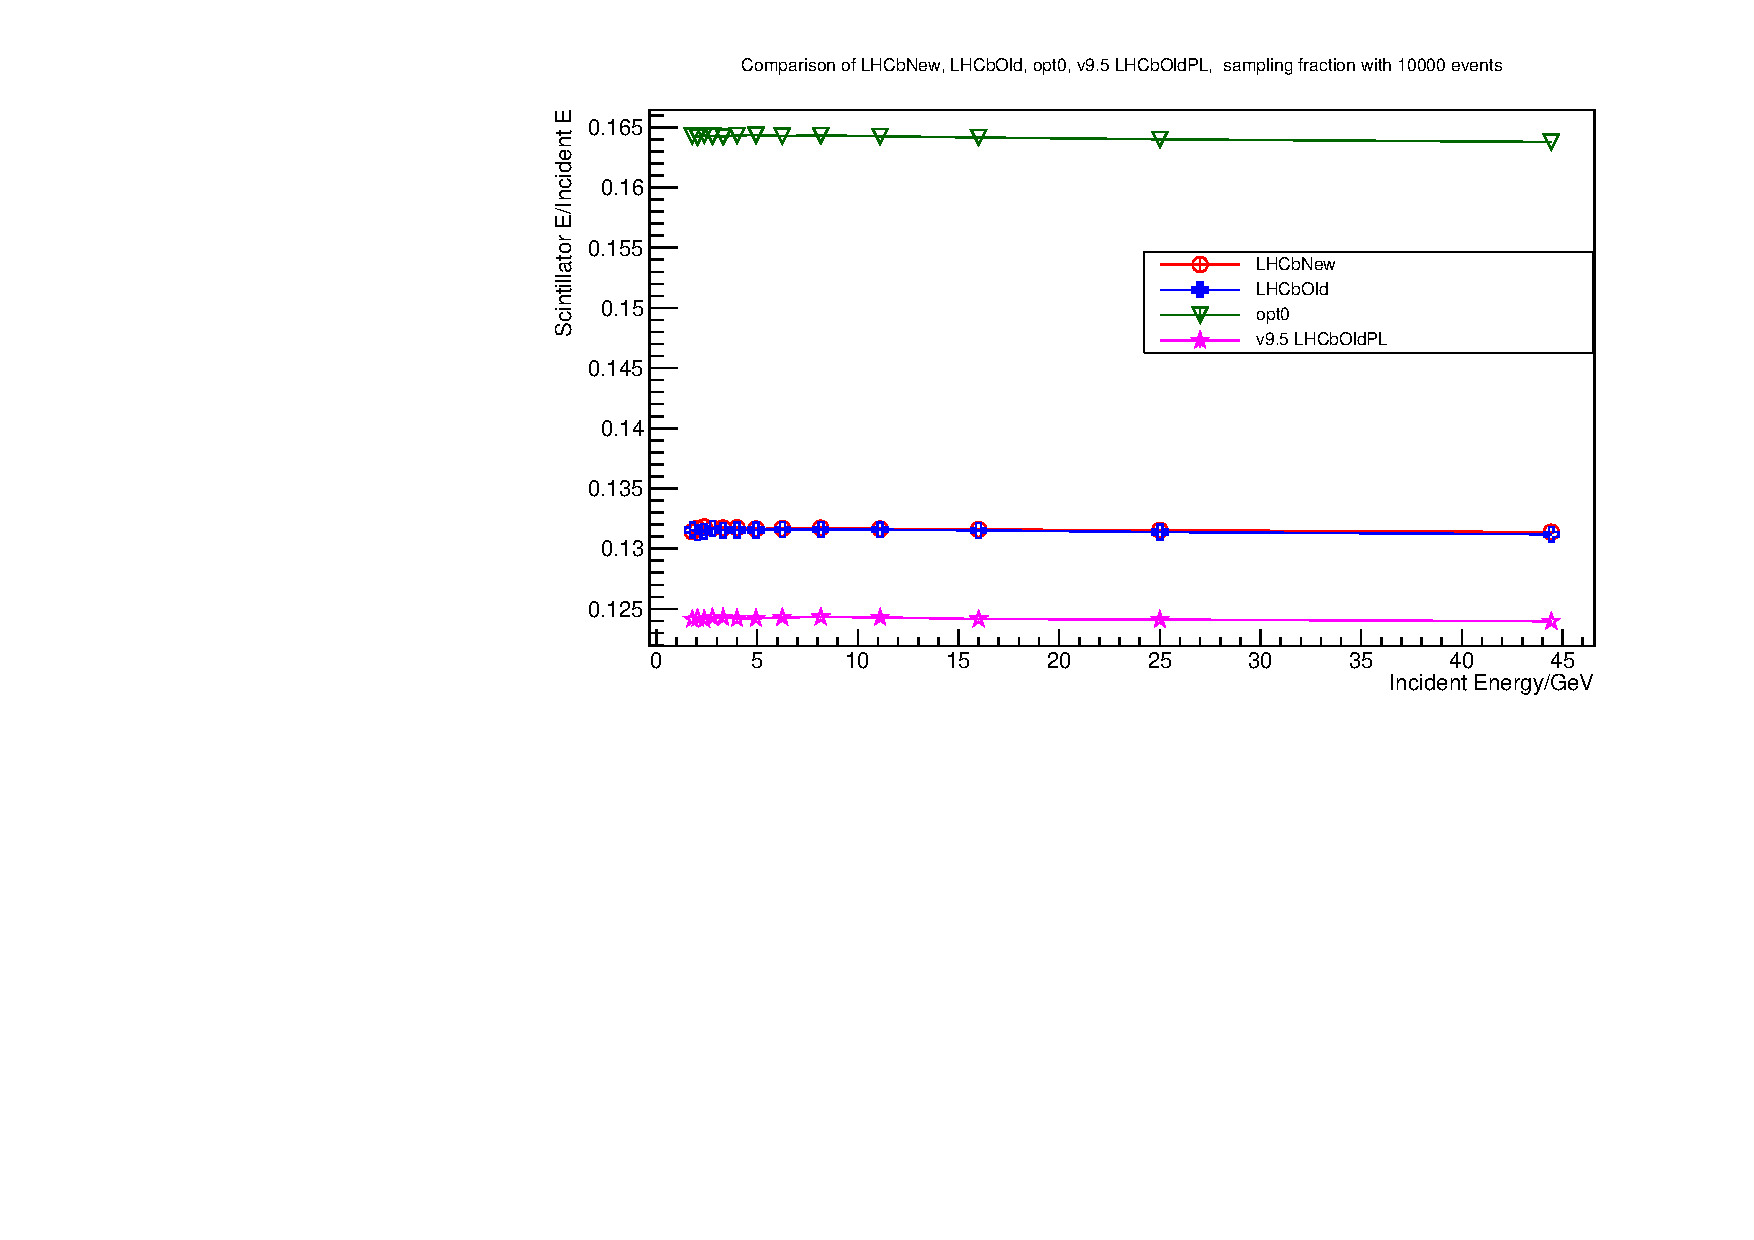
\includegraphics[width=\textwidth]{ProgressSF.pdf}
  \caption{Sampling fraction of the ECAL as a function of energy}
  \label{fig:ProgressSF}
\end{figure}
%\begin{figure}[h]
 % \centering
 % 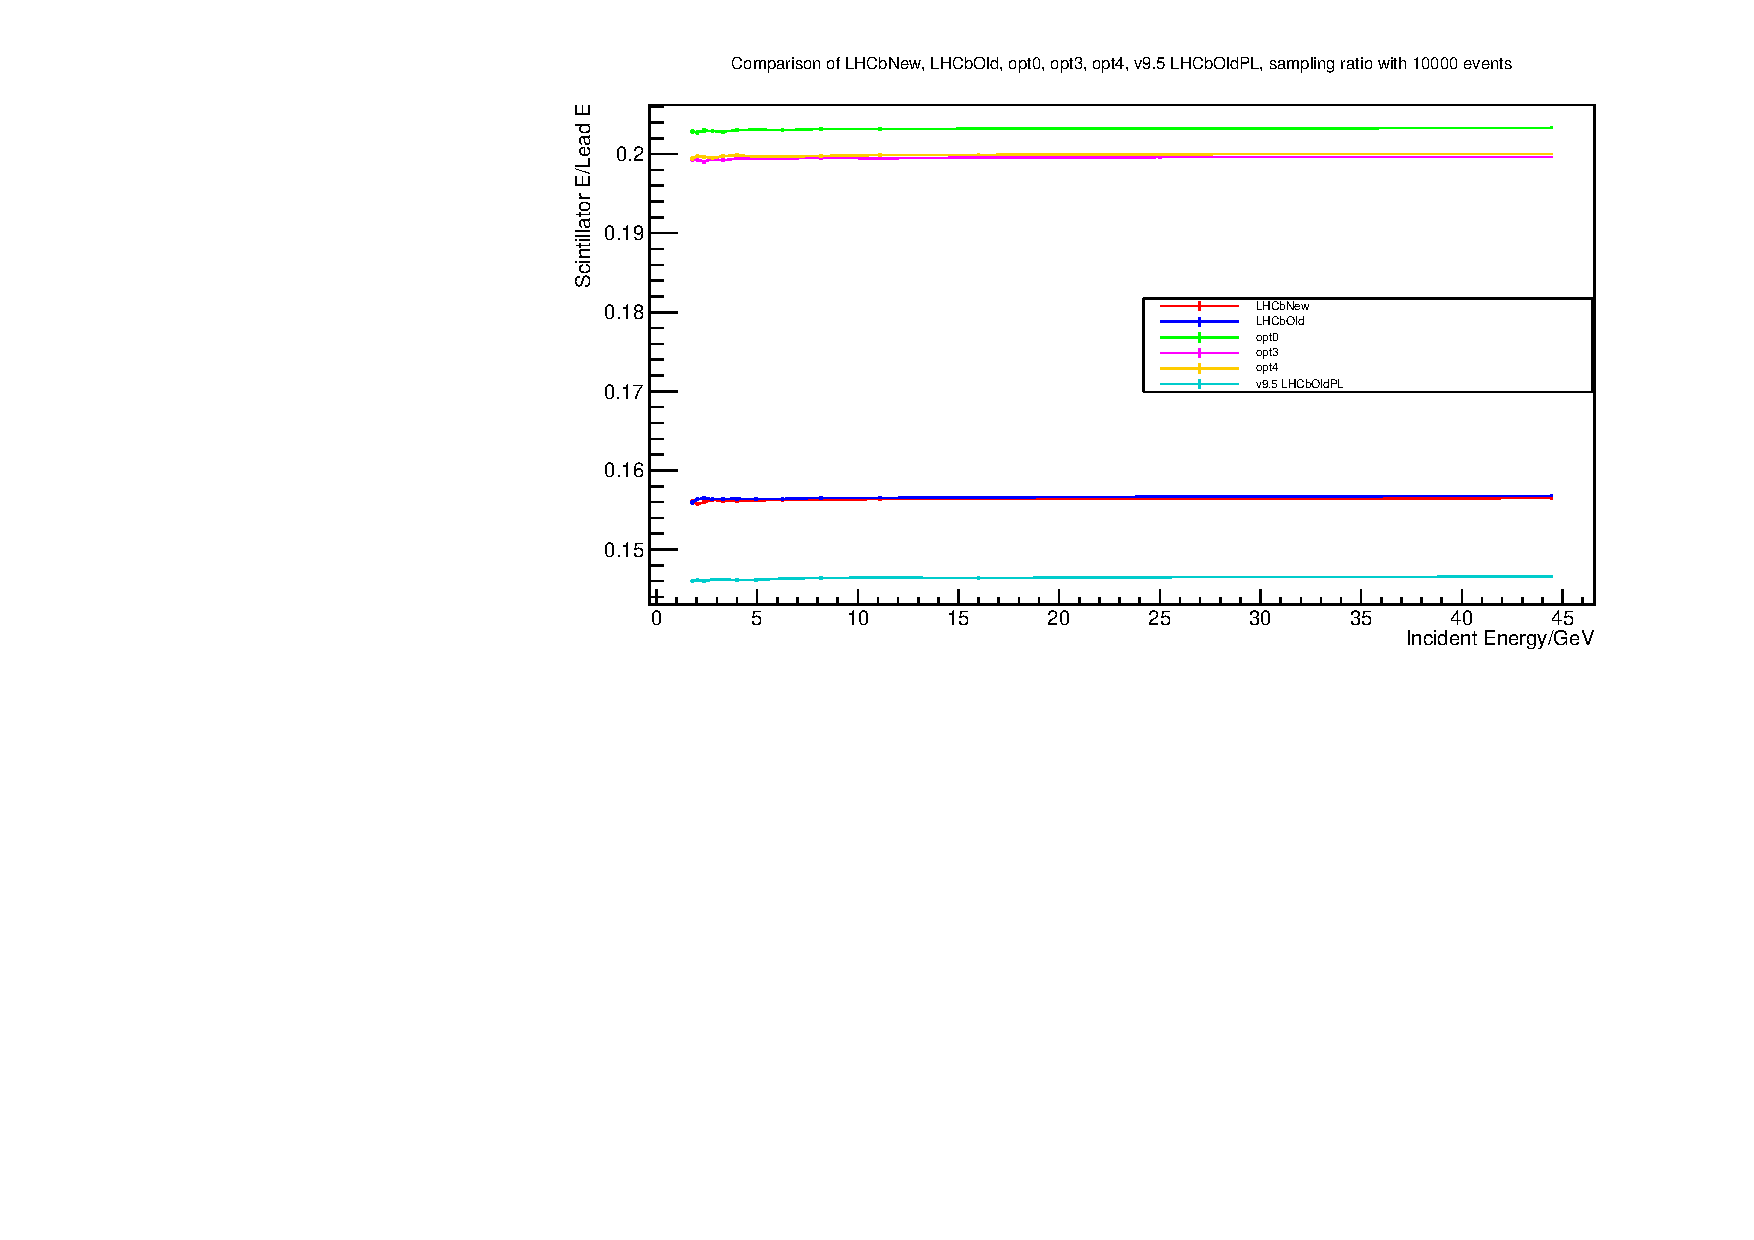
\includegraphics[width=\textwidth]{ProgressRatio.pdf}
 % \caption{Sampling ratio of the ECAL as a function of energy}
  %\label{fig:ProgressRatio}
%\end{figure}

Figure \ref{fig:ProgressSF} also shows that moving to \geant v9.6 has made progress towards more accurate results for the \lhcb private PLs.  Unlike the fractional resolution, however, the LHCbOld PL and LHCbNew PL sampling fractions are within uncertainties of each other at the majority of energies.  Therefore, for the purposes of choosing a new EM PL they have to be considered to be equally as accurate.

\begin{figure}[h]
  \centering
  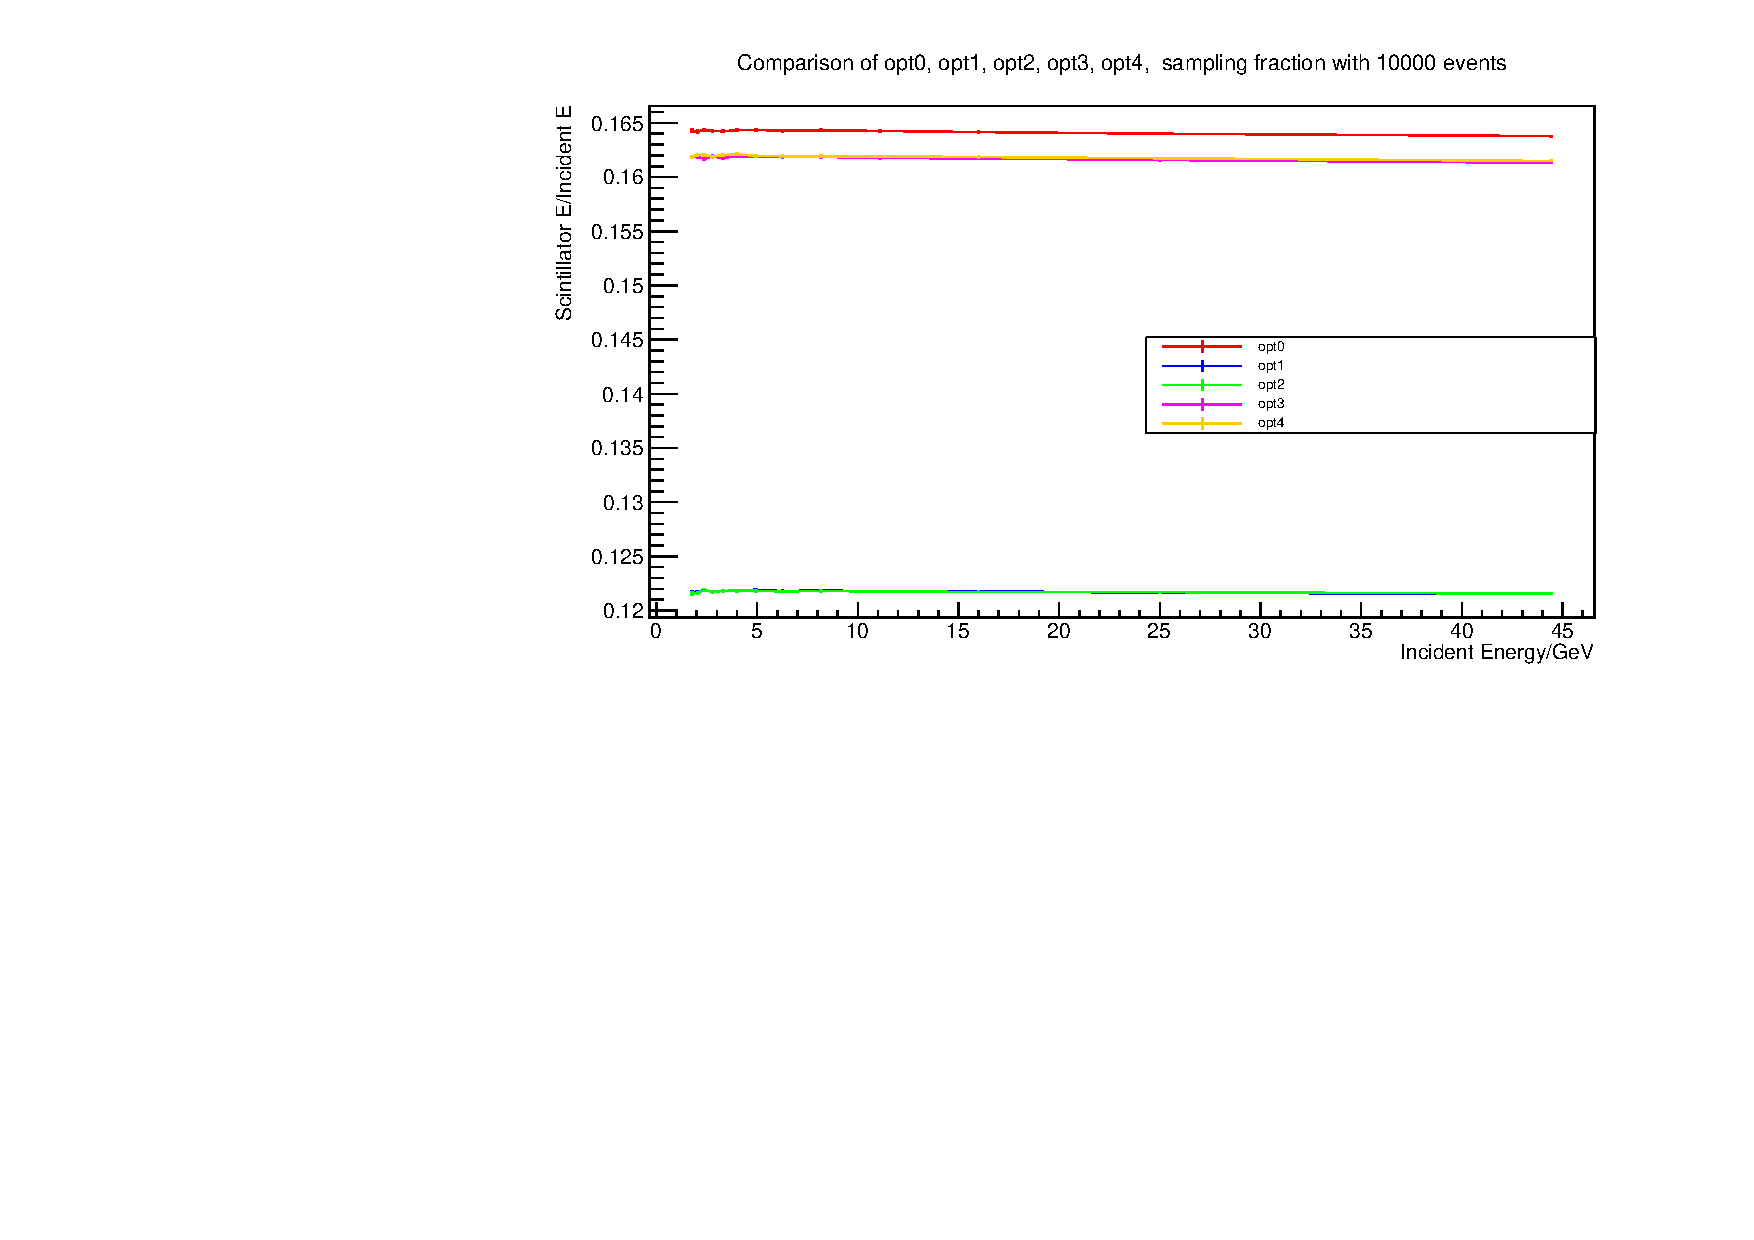
\includegraphics[width=\textwidth]{BoxSF.pdf}
  \caption{Comparison of sampling fractions from \geant supplied PLs}
  \label{fig:BoxSF}
\end{figure}
%\begin{figure}[h]
 % \centering
  %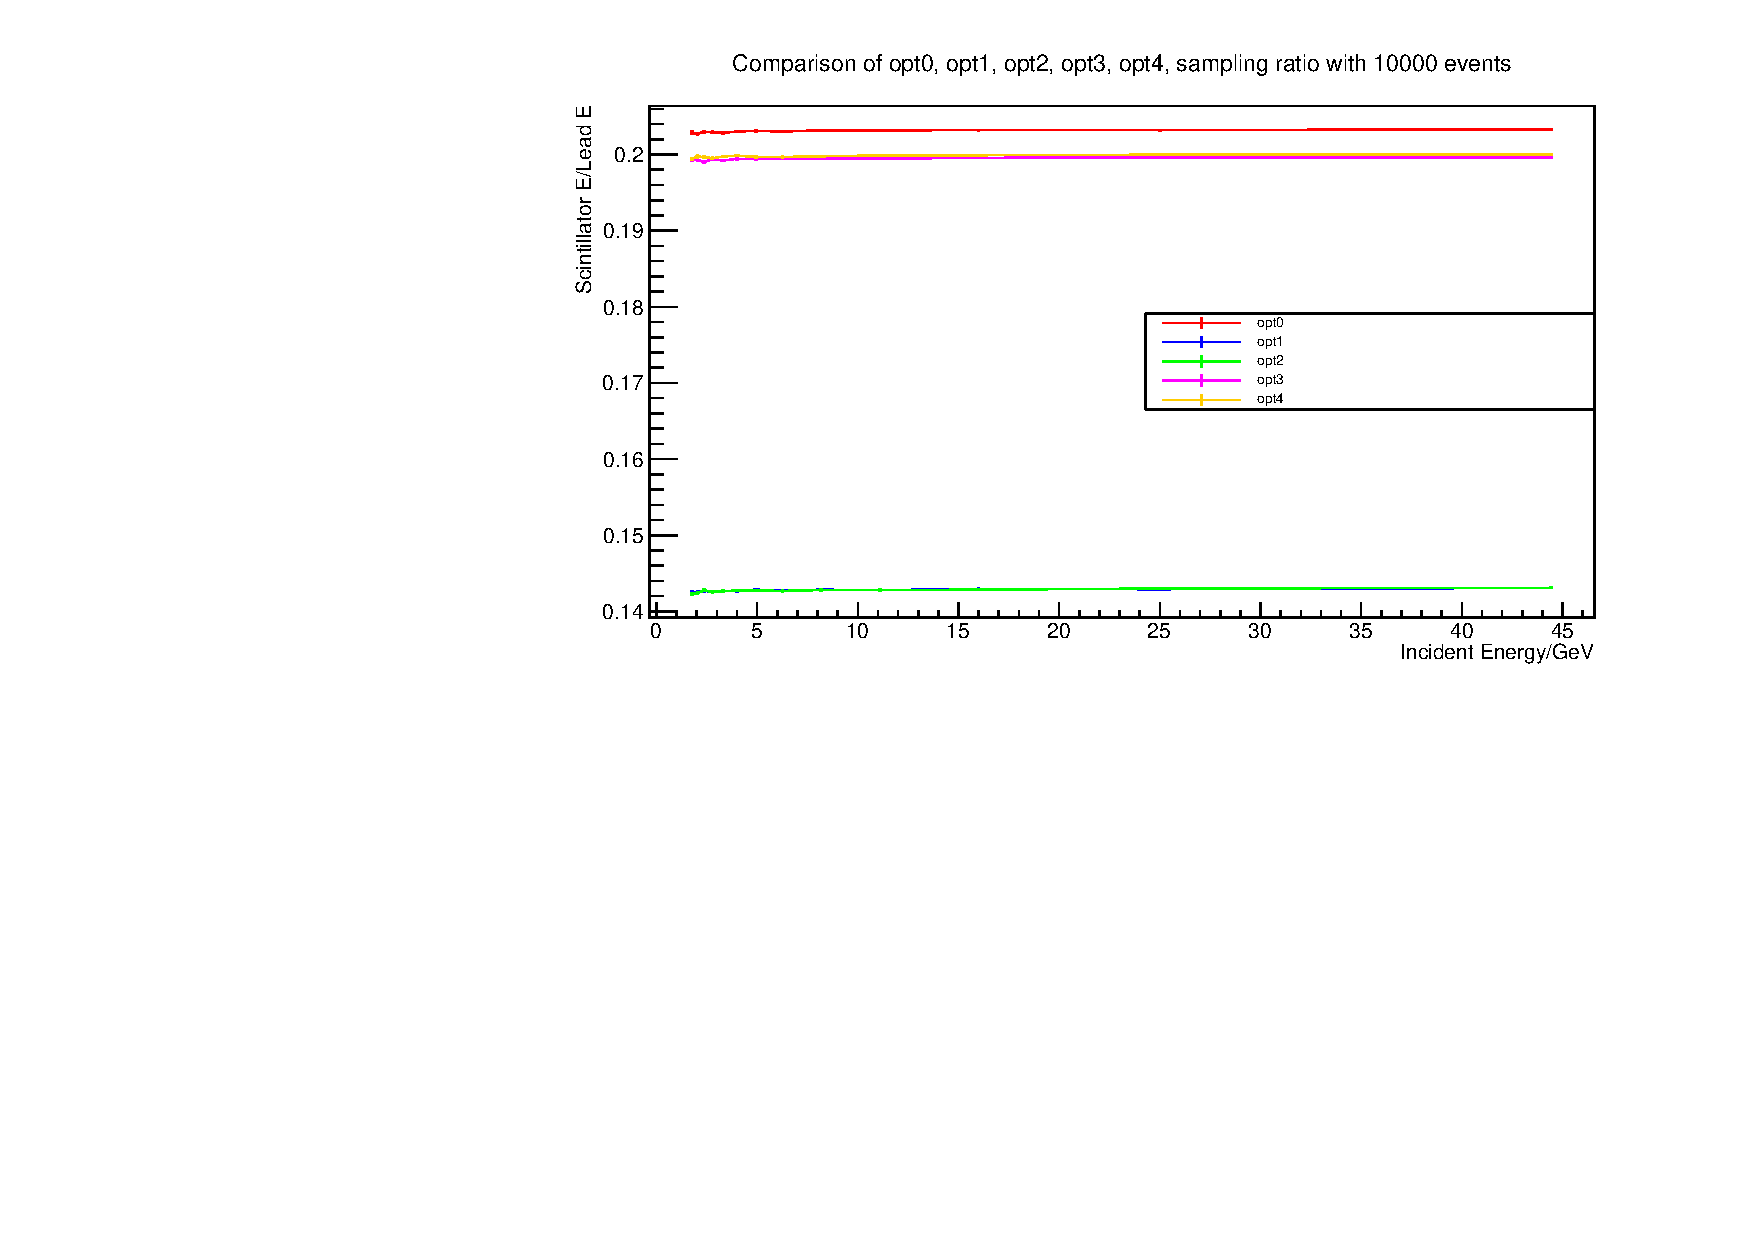
\includegraphics[width=\textwidth]{BoxRatio.pdf}
  %\caption{Comparison of sampling ratio from \geant supplied PLs}
  %\label{fig:BoxRatio}
%\end{figure}
Figure \ref{fig:BoxSF} shows that the \textit{opt1} and \textit{opt2} physics lists produce very similar results.  However, they are very different to the results produced by the more accurate PLs that do not use a simplified multiple scattering model.  The same effect is observed under \geant internal tests, which is a useful cross check\cite{1742-6596-219-3-032045}.

These results shows that using the \textit{fMimimal} option in the multiple scattering model has a large inpact on the amount of energy deposited, which is a quantity one would not intuitively expect to be effected by multiple scattering.  However, as described in section \ref{sec:steps}, the length of a step taken before all particle properties are re calculated is the minimium of the step length for all physics processes.  Consequently, the distance between positions where the energy loss is sampled can be effected by multiple scattering even though it plays no role in the energy loss calculations.  With \textit{fMinimal} applied the step lengths calculated for the multiple scattering process are longer, meaning that in some cases the step length used is also longer.  Therefore, energy losses are sampled less often which decreases the accuracy of the simulation.

\subsubsection{Simple Calorimeter Test Conclusions}
\label{ref:CaloConclusions}
Firstly, a significant discrepancy in fractional resolution and sampling fraction of a model \lhcb ECAL has been observed between \geant v9.5 and v9.6.  Consequently, the \lhcb calorimeter group will have to re calibrate the ECAL for the new release of \gauss. This discrepancy is believed to be a result of the new \geant version depositing more energy in scintillator and less in lead layers, most likely as a reuslt of updates to the multiple scattering models used.  This discrepancy has resulted in the \geant collaboration suggesting the \lhcb EM PL should be updated to a new multiple scattering model.  The studies in section \ref{sec:Comaprison of PL} show that updating the \lhcb EM PL to follow the \textit{emstandard opt1} PL actually increases this discrepancy. The stochastic component of the fractional resolution parameterisation changes from $0.922 \pm 0.0003$ with the old \lhcb PL to $0.910\pm 0.002$ with the updated \lhcb PL. However, the fractional resolution study using the most accurate PL available for the energy ranges considered here (\textit{emstandard opt0}) yields a stochastic term of $0.794\pm0.0002$.  Therefore, updating the \lhcb PL would cause progression of results towards a more accurate measurement.

A choice of PL has to be made for the next release of \gauss.  Throughout this study CPU time was monitored because it is a valuable and limited resource in particle physics.  It was noted that there was a siginificant increase in CPU time required when a PL without a simplified multiple scattering model was used. This increase varied from a factor of 2, to a factor of 6 compared to v9.5.  Other studies have shown that approximately $45\%$ of the time taken to simulate an event in \gauss is spent simulating the electromagnetic shower.  Therefore, even a factor of 2 increase in CPU time is not feasible.  The consequences of this are that only \textit{emstandard opt1}, \textit{emstandard opt2}, \textit{LHCbOld} and \textit{LHCbNew} are viable choices for the new PL.

Section \ref{sec:Comaprison of PL} shows that \textit{LHCbNew} produces results closest to a non simplified multiple scattering models for fractional resolution studies.  Moreover, \textit{LHCbNew} and \textit{LHCbOld} both show closer agreement to the unbias PLs for sampling fractions and sampling resolutions compared to \textit{opt1} and \textit{opt2}.  Therefore, either of the \lhcb private PLs were deemed to be a better choice. 

Furthermore, \lhcb has previously experienced issues with the agreement between data and MC for the impact parameter resolution.  The conclusion of an extensive investigation into this issue was to use the PL described here as \textit{LHCbOld}.  Therefore, it was decided that the new PL should stay as close as possible to \textit{LHCbOld} to avoid introducing disagreements between data and MC elsewhere in the detector simulation.  Therefore, it was decided that the updated \lhcb private PL \textit{LHCbNew} should be adopted as the new EM PL.

%TODO cite geant4 testing.

%TODO cite jimmys thesis . 


%Figure \ref{fig:BoxPLStraightFR} shows 
%Simple Calorimeter Test
%----Calorimetry Background
%----Comparison of Geant4 versions
%---------Resolution investigations
%---------Sampling fraction investigations
%---------Geant4 version comparison results discussion
%----Physics List investigations
%---------Fractional Resolution
%---------Sampling Fraction Results
%---------Results Discussion

%MSC
%--results
\clearpage

\subsection{Multiple Scattering Test}
\label{sec:Multiple Scattering Test}
Since the multiple scattering model has been updated in the EM PL, it was decided a direct study of multiple scattering was necessary.  When a charged particle traverses a material there is a non-zero probability that it will undergo elastic coulomb scattering from a nuclei within the material.  The differential cross section for this process is given by,
\begin{equation}
  \label{eq:Rutherford}
  \frac{d\sigma}{d\Omega}=\big(\frac{1}{4\pi\epsilon_0}\big)^2\frac{z^2e^4}{M^2c^4\beta^4}\frac{1}{sin^4(\theta/2)}
  \end{equation}
where $\Omega$ is solid angle, z is the atomic number of the material, M is the mass of the charged particle and $\theta$ is the angle through which the charged particle is scattered\cite{eisberg1974quantum}.

Except for cases where the scattering material is a very thin film, the charged particle will scatter multiple times before exiting the material.  Hence, multiple coulomb scattering occurs which is more commonly known as just multiple scattering. The net effect is a lateral displacement as well as a scattering angle, as depicted in Figure \ref{fig:MSCPDG}.  In this case a statistical treatment has to be used to obtain a distibrution for the scattering angle, which is defined as $\theta$ in Figure \ref{fig:MSCPDG}. This was first carried out successfully by Moliere theory, which has been shown to give very good agreement with data over a wide range of particles, materials and energies \cite{PhysRev.89.1256,Gottschalk1993467}.  Several other theories have been shown to produce consistent results but the most complete is Lewis theory, which also provides moments for the spatial displacement distribution \cite{PhysRev.78.526}.

Both the Moliere and Lewis theory give a scattering angle distribution that is gaussian for the central $98\%$ of scattering angle values, but the tails of the distibrution fall off slower than a gaussian due to the $\frac{1}{sin^4(\theta/2)}$ term in equation \ref{eq:Rutherford}.  The width of the central gaussian is defined as $\theta_0$ which can be approximated by the Highland formula,
\begin{equation}
  \label{eq:Highland}
  \theta_0=\frac{14.1MeV}{pv}z\sqrt{\frac{L}{L_R}}\big[1+\frac{1}{9}log_{10}\big(\frac{L}{L_R}\big)\big]
\end{equation}
where p is the incident particles momentum, v is the incdient particles velocity, L is the length of the material and $L_r$ is the radiation length of the material.  This formula is an emperical formula that arises from fits to moliere theory \cite{Highland1975497}.

\begin{figure}[h]
  \centering
  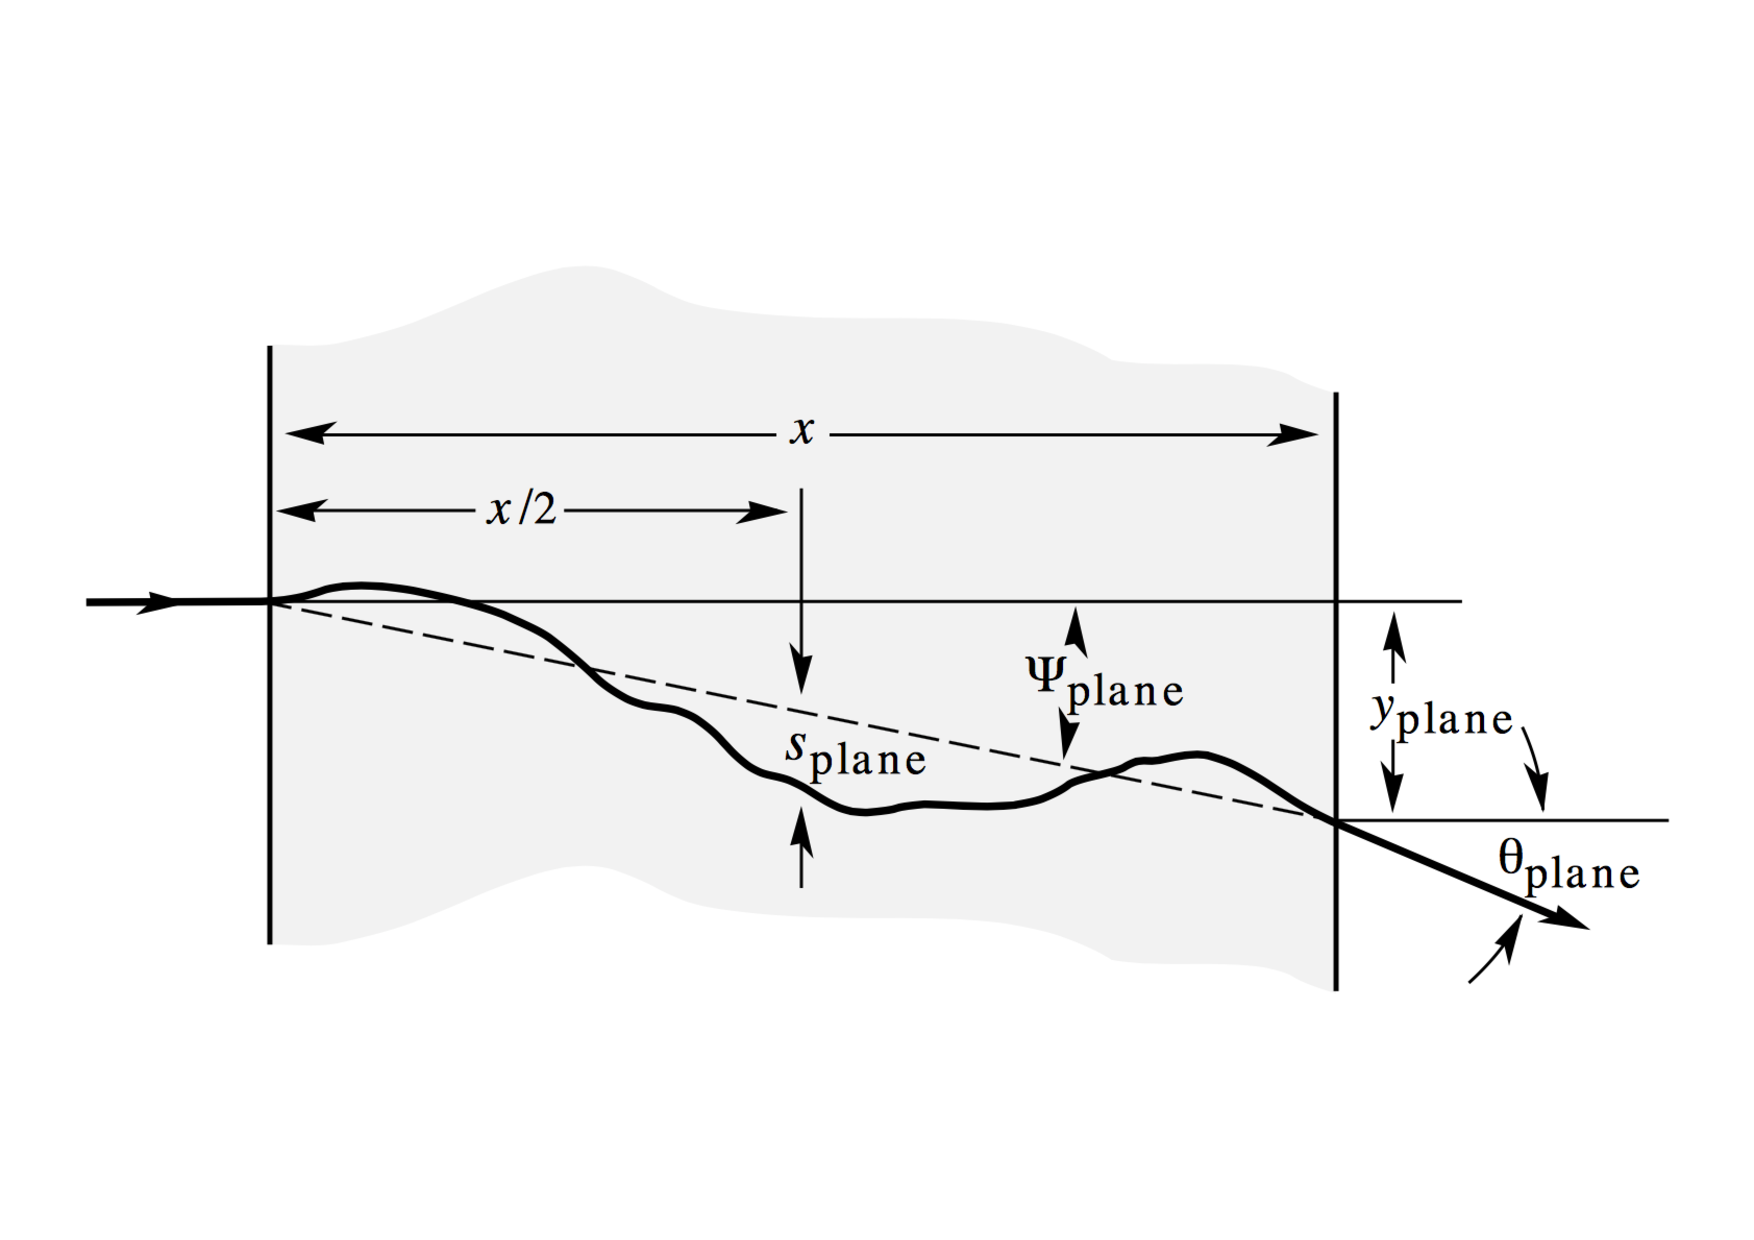
\includegraphics[width=\textwidth]{MSCPDG.pdf}
  \caption{A diagram showing the lateral displacement and angular dispersion when a charged particles traverses a medium.}
  \label{fig:MSCPDG}
\end{figure}

When one simulates multiple scattering, in a similar way to the theoretical models, it is rarely possible to simulate every individual collision.  It is only possible if the number of scatters is small and large amount of CPU time is available.  For the latter reason, this type of simulation based on simulating every single scatter was not implemented until 2005.  Unfortuantely, there is still a limited number of applications where this is a viable option.  The \textit{UrbanMsc} models get around this by using  a ``condensed'' simulation of multiple scattering, which involves simulating a step of the particles path at a time and applying net effects at the end of each step \cite{Urbàn:592633}.  More sepcifically, the angle through which the particle has been scattered and the lateral displacement are applied at the end of each step as part of the multiple scattering simulation.  The scattering angle is sampled from distributions calculated using Lewis theory but no theory of a full displacement distribution exists.  Therefore, \geant uses its own, non-exact, algorithms to calculate the lateral displacement after each step %TODO cite physics reference manual.

Another approach to simulating multiple scattering, that has been implemented more recently, is to use a ``mixed'' approach.  This involves sampling scatterers, where the scattering angle $\theta$ is below a threshold $\theta_{max}$, in a similar way to the ``condensed'' approach discussed previously.  However, if the scattering angle is above $\theta_{max}$ then a single scattering approach is used.  This is implemented in \geant as the \textit{WentzelVI} model.

In moving to the new EM PL the multiple scattering model for electrons and positrons has changed from \textit{UrbanMsc95} to \textit{WentzelVI} above 100MeV, therefore the model has moved from being condensed to mixed.  However, below 100MeV the model has moved from \textit{UrbanMsc95} to the older \textit{UrbanMsc93} which involves some subtle changes. %TODO write more.

To carry out a direct investigation of multiple scattering and how it is effected by these changes, the \geant example TestEm5 was used. The example provides the facility to fire particles into a square sheet of material at normal incidence and study the angle of the scattered particle, to the normal, as it exits the material on the other side. A diagram of this is shown in Figure \ref{fig:TestDiam}.  The type of material used, the width of the material and thickness of the material can all be specified. In this case the setup used was a $300 \mu m$ thick sheet of silicon designed to model the \lhcb VELO as closely as possible, because this is the area of the detector where the most precise tracking measurements sensitive to multiple scattering take place.
\begin{figure}[h]
  \centering
  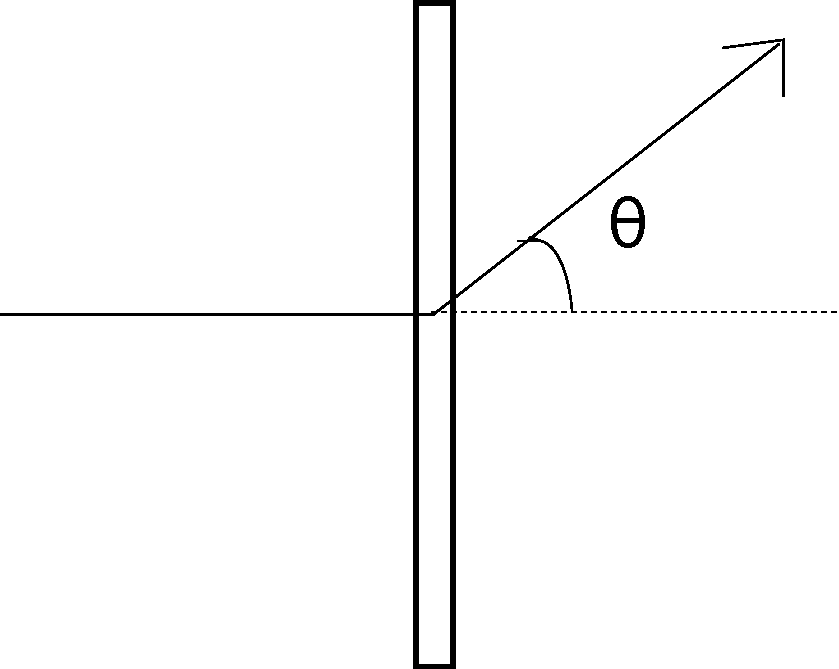
\includegraphics[width=0.7\textwidth]{TestEm5Diag.pdf}
  \caption{A diagram showing the setup of TestEm5.  $\theta$ is the angle under investigation by this test}
  \label{fig:TestDiam}
\end{figure}

The aim of this investigation was to measure the parameter $\theta_0$ of the scattered particles angular distribtuion for electrons at a range of energies and use it as a comparison tool between PL configurations and \geant versions.  The \geant example is pre-configured to calculate $\theta_0$ by taking the standard deviation of the central $98\%$ of values after each run.  However, no estimation of the uncertainty is performed by the example. As the time to simulate 10000 electrons with this minimal geometry was <1 second, the simulation was re-run 10000 times at each energy and configuration.  $\theta_0$ was recorded for each run and the end result was assigned as the mean of all runs with an uncertainty given by the RMS of all 10000 runs.

The energies chosen for this investigation were 1,2,3,4,5,7,9,12,15,20,25,30 and 40 GeV as these were considered representative of the expected electron energies at \lhcb. The following configurations were tested with these energies: \geant version 9.5 with the \textit{LHCbOld} PL and version 9.6 with \textit{LHCbNew} PL and verision 9.6 \textit{LHCbOld} PL.  These were chosen because it allows a direct comparison between the old release of \geant and the new release of \geant to be made.  v9.6 \textit{LHCbOld} was included to offer insight into the cause of any discrepancies observed.

\subsubsection{Results}
\label{sec:MscResults}
The results for $\theta_0$ from running the simulation with v9.6 \textit{LHCbOld} and \textit{LHCbNew} were divided by the results from running the simulation with v9.5 and \textit{LHCbOld} to make a direct comparison with the previous release of \geant.
\begin{figure}[h]
  \centering
  \includegraphics[width=\textwidth]{theta0.pdf}
  \caption{$\theta_0$ as a function of energy normalised to \geant v9.5 \textit{LHCbOld}}
  \label{fig:theta0}
\end{figure}

Firstly, and most imporatantly, Figure \ref{fig:theta} shows that the width of the angular distribution from the new version of \geant with the new physics list has increased by $4-6\%$ compared to what was used in the previous release of \geant.  The statistical significance of this change varies from $5.77\sigma$ at 1GeV to $7.95\sigma$ at 40GeV, meaning there is no doubt that this is due to a systematic change in the simulation process.

Secondly, Figure \ref{fig:theta} also shows that this change in $\theta_0$ must be largely attributed to the changes made to the multiple scattering model rather than moving to a new version of \geant.  Although the results with the new version of \geant and the old PL are systematiclly $0.5-1.3\%$ and upto $1.7\sigma$ larger, this is still considerably smaller than when the new PL is used with v9.6.

\subsubsection{Conclusions}
\label{sec:Conclusions}
Clearly the angular distribution with the new \geant version and PL has changed when a \lhcb VELO like situation is considered.  Unfortuantely, due to limitations of the \geant example it is only possible to consider scattering from one sheet of silicon which is not completely representative of the entire VELO system (see section detector).  Therefore a full detector simulation using \gauss is required to study this discrepancy and, importantly, the effect on the impact parameter resolution.  This simulation will be carried out by the \lhcb VELO group when the new release of \gauss is made.
%TODO ref detector section.

\clearpage


% $Id: introduction.tex 65669 2015-01-09 14:55:20Z tgershon $
\section{Investigation of $\Bd \rightarrow \Kstar(892) \etaz$}
\label{sec:Analysis}
%motivation and stuff here TODO
The intention of this analysis is to use the decay \Bd \to \Kstar \etaz as a control channel in the search for \Lb \to \proton \Km \etaz.  As of yet a \Lb baryon has never been observed to decay to a final state involving an \etapr or \etaz particle.  However, evidence for the decay \Lb \to \Lz\etaz at the level of $3\sigma$ has been observed by \lhcb \cite{LHCb-PAPER-2015-019}. Unfortunately, the search for \Lb \to \Lz \etaz suffered from low trigger efficiencies due to the long lived nature of the \Lz baryon. However if the \Lb instead deacys to a short lived \Lz resonance and an \etaz particle, trigger efficiencies are expected to be higher.  If this intermediate resonance is the $\Lz^{*}$(1520) or heavier, it can then decay to \proton \Km giving the final state that is the subject of this analysis.  The dominant feynman diagram for this decay is shown in Figure \ref{fig:feynman}, where the b\to s transition is mediated by an electroweak loop.
\begin{figure}[h]
  \centering
  \begin{subfigure}[b]{0.49\textwidth}
    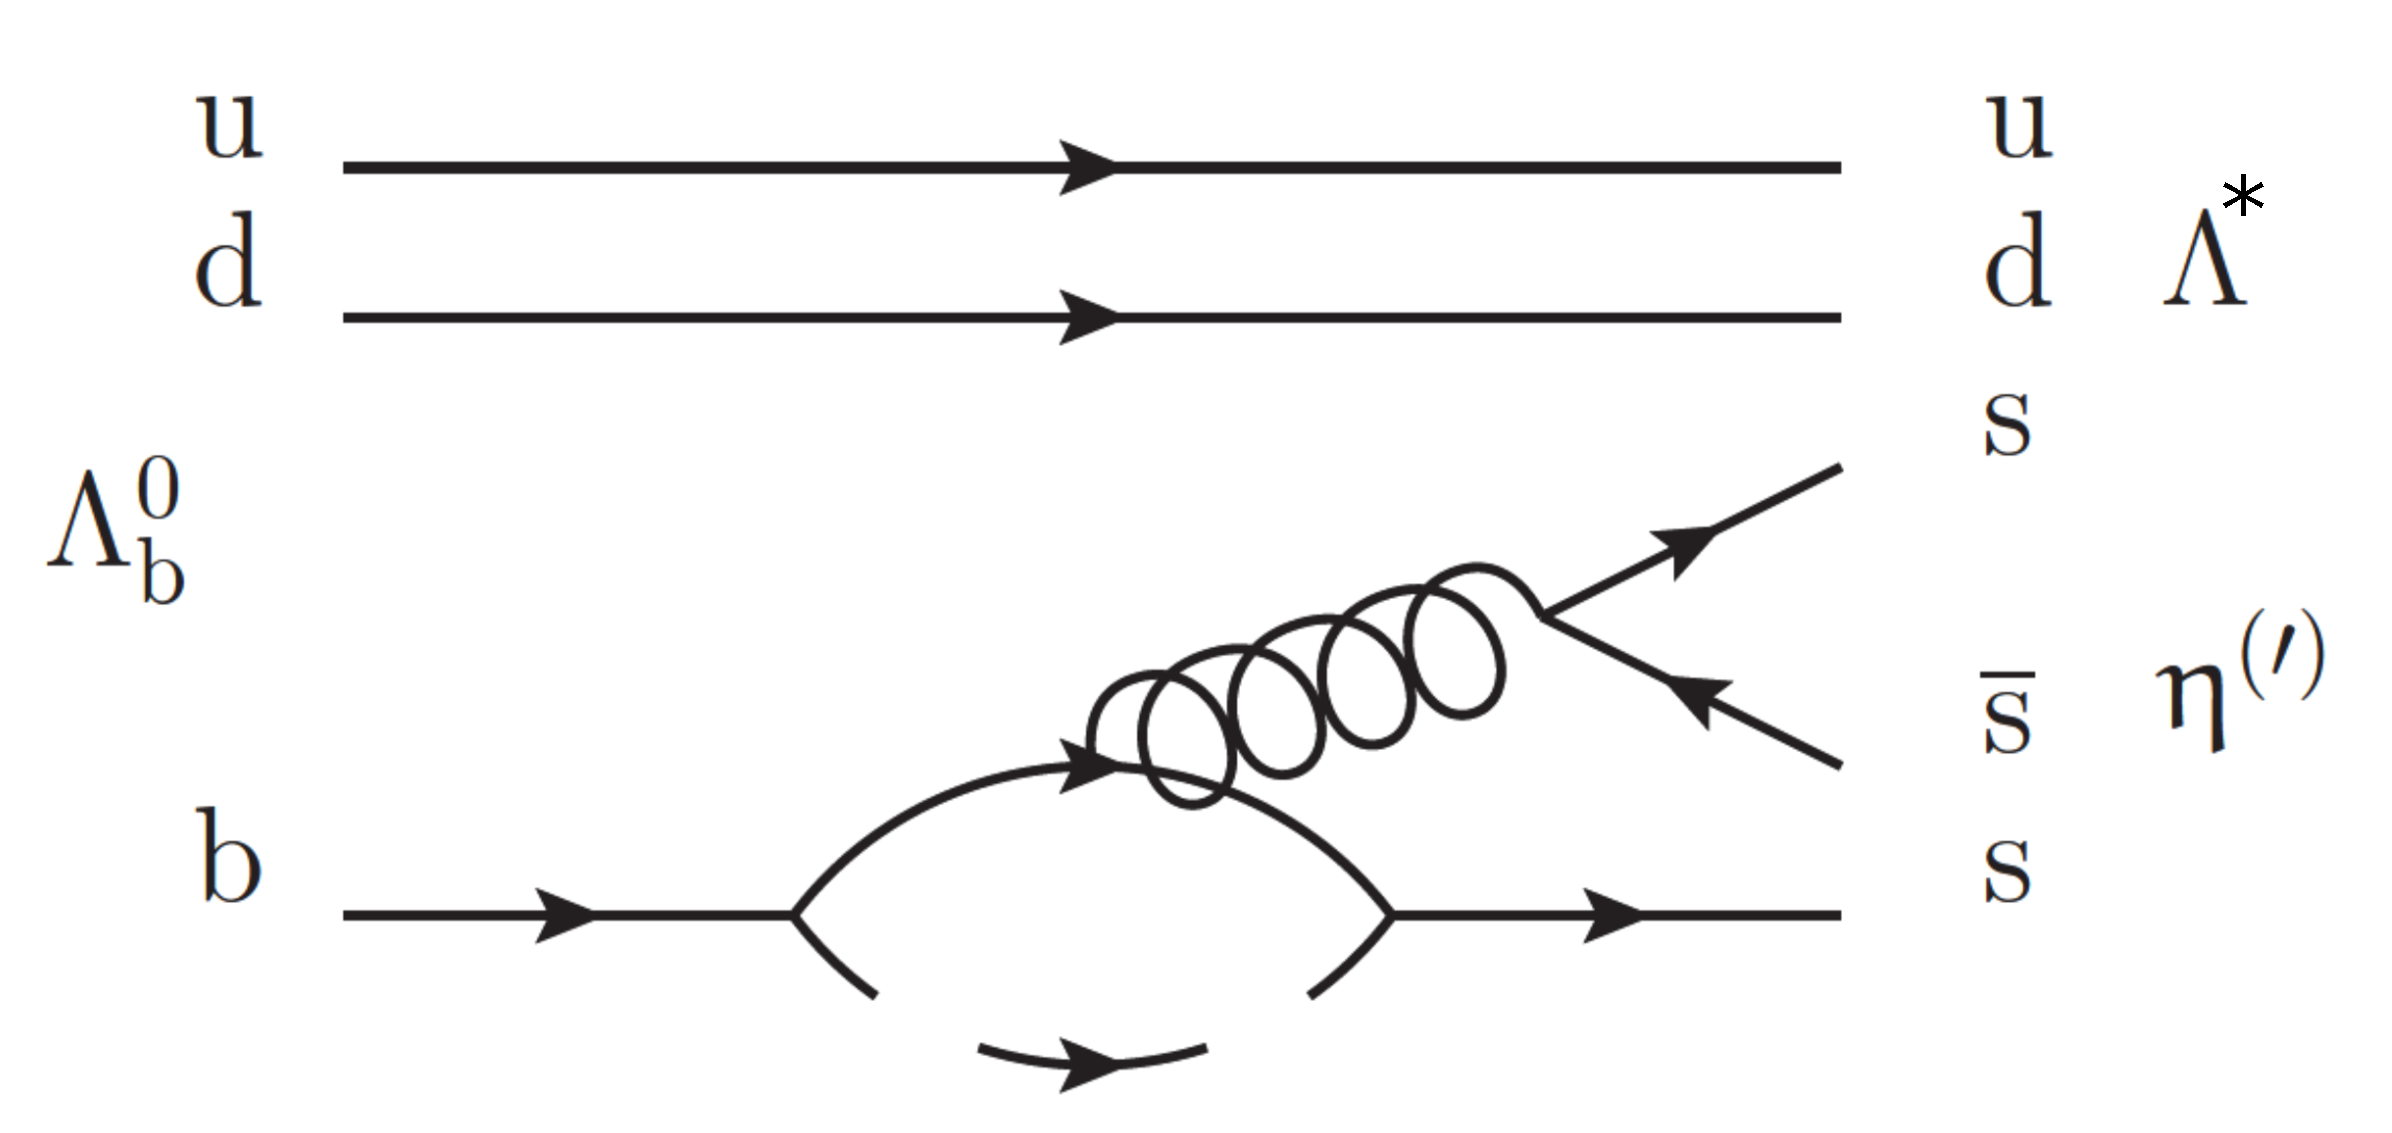
\includegraphics[width=\textwidth]{lambdaresfeynman.pdf}
    \caption{ \Lb decaying to $\Lz^{*}$ and $\etaz^{(')}$ }
    \label{fig:Initial}
  \end{subfigure}
  \begin{subfigure}[b]{0.49\textwidth}
    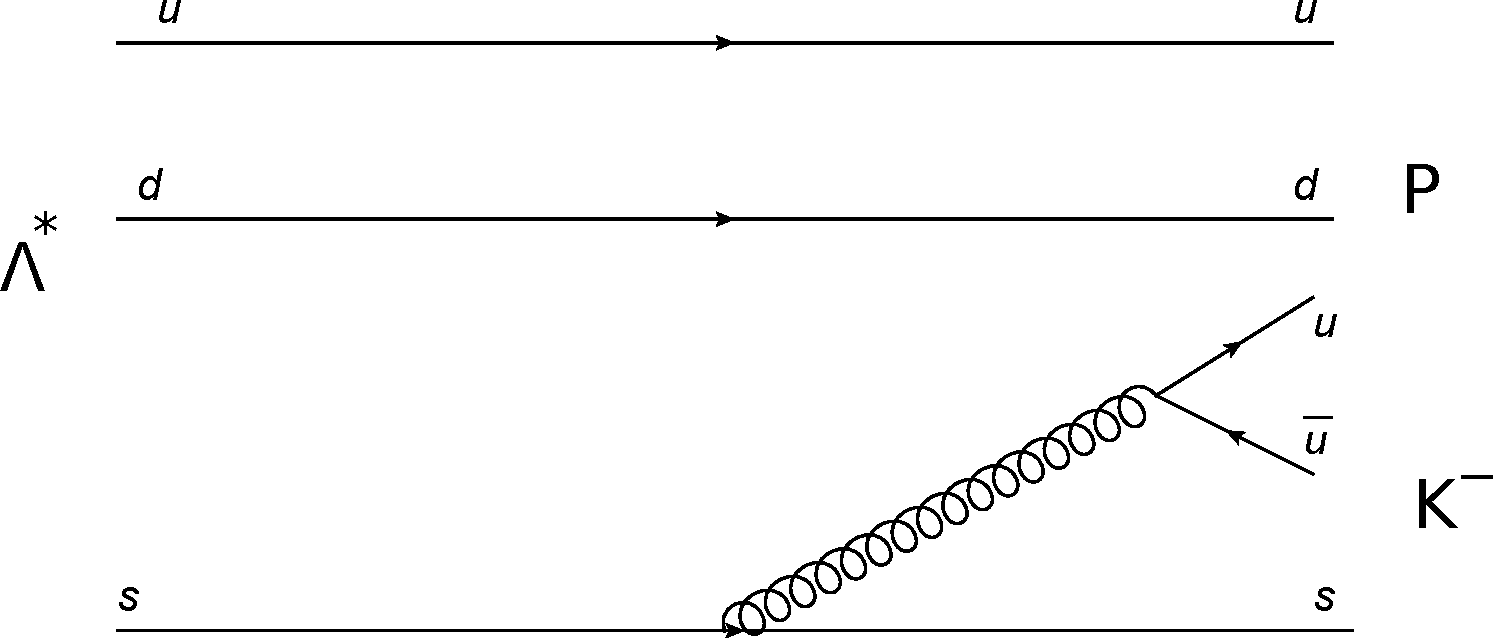
\includegraphics[width=\textwidth]{LambdaDecFeyn.pdf}
    \caption{$\Lz^{*}$ decaying to \proton \Km.}
    \label{fig:next}
  \end{subfigure}
  \label{fig:feynman}
  \caption{Feynman diagrams showing how the rare decay often proceeds.}
  \end{figure}

In order to measure (or set a limit on) the branching fraction of \Lb \to \proton \Km the number of events observed has to be measured relative to the yield of a decay with a know branching fraction.  This is because it is incredibly difficult to measure the efficiency of the detector well enough to make an absolute measurement.  \Bd \to \Kstar \etaz is a good control channel for this search because it has only a pion/proton difference in the final state meaning minimal efficiency differences between the decays will need to accounted for when the relative branching fraction is calculated.  The world average of the branching fraction is currently $1.59\pm0.10 \times10^{-5}$, which means the uncertainty on this branching fraction should not be dominant in the measurement of the branching fraction for the rare mode.  This branching fraction measurement has been made, most recently, at  \babar and \belle\cite{Wang:2007rzb,Aubert:2006fj}.

The intention of this analysis is to use the full $3fb^{-1}$ dataset collected by \lhcb in run I of the LHC.  However, the $1fb^{-1}$ of data collected at a 7TeV centre of mass energy (CoM) and the $2fb^{-1}$ of data collected at an 8TeV centre of mass energy will be treated seperateley at least for the selection stage of this analysis.  This is because the differences in kinematic variables between these two CoM energies would make a common selection for both sub-optimal. So far only the $2fb^{-1}$ of 8TeV data has been considered, therefore all results in this report are based on that dataset.

\subsection{Decay Reconstruction}
\label{sec:Decay Reconstruction}
The \Kstar will be reconstructed in the channel $\Kstar \to \Kp\pim$ which has a branching fraction of $99.901\pm0.009\%$ \cite{PDG2014}.  The \etaz will be reconstructed in the channel $\etaz \to \pip\pim\piz$ where the \piz decays to 2 photons, which has a combined branching fraction of $21.83\pm0.28\%$\cite{PDG2014}.  This is not the dominant decay mode of the \etaz particle but the 2 decay modes with higher branching fractions contain only neutral particles in the final state.  This means there is no tracking information available and the \lhcb calorimeter (unlike the \atlas calorimeter) does not provide any directional information for the photons it detects.  Consequently, reconstruction efficiencies for all neutral final states are significantly lower and backgrounds are higher, which makes the \pip\pim\piz channel the optimal choice.  

Each of the final state particles in the decay chain are assigned a mass hypothesis based on information from all of the \lhcb sub detectors before being combined to form their respective mother particles.  The properties of the mother particle (e.g Energy, momentum, flight distance) are then determined with a fit to the daughter particles;   the $\chi^2$ of this fit can then aid the choice of candidate decays.

The combination of particles to form a \Bd candidate described is all done by the \lhcb reconstruction packages and the initial, loose, selection of \Bd candidates is based on this reconstruction. However, a better mass resolution can be achieved by refitting the entire decay tree of \Bd candidates whilst applying extra constraints.  This technique was first used by the \babar and is practically implemented with a Kalman fitter\cite{Hulsbergen:2005pu}.  Most commonly, any intermediate daughter particles are constrained to have their known masses and all tracks are constrained to come from the position where the hard pp interaction took place (primary vertex).  In this analysis all daughter particles are constrained to come from the primary vertex and the \etaz mass is constrained to the current world average ($547.826\pm0.018MeV$)\cite{PDG2014}.  The \Kstar mass is not constrained because it is a wide resonance; the natrual width of the \Kstar is around 50MeV.  It is impossible to reconstruct a particle with a better resolution than what is dictated by it's natural width.  Consequently, one can expect correctly reconstructed \Kstar particles to still have a mass a considerable distance from the PDG value.  Therefore, constraining the \Kstar candidate to its PDG value can bias the refitted \Bd mass.

\subsection{Event Selection}
\label{sec:Selection}

The first stage of any analysis is selecting a subset of the \lhcb dataset that contains a high purity of events of interest to the analysis.  Essentially, one has to mimise the number of background events that pass a set of selection criteria whilst keeping as many signal events as possible. These selection criteria are composed of several stages.

\subsubsection{Stripping Selection}
\label{sec:Stripping}
As the data collected by \lhcb in run I is of the order of 10s of Petabytes it is impossible for every user to start with the full dataset.  Therefore, loose selection criteria need to be applied to the full dataset to produce a subset of data that can be worked with.  A set of these loose selection criteria are refered to as a stripping line, some of which are quite general (e.g dimuon final state) whereas others are for a specific analysis.  The amount of CPU time taken to run over the full run I dataset is very large, therefore stripping takes place when the data is taken and then incremental re-strippings take place no more than a few times a year.  The stripping process is always run centrally.
%TODO check how to make a stripping line
The cuts that go into a stripping line are determined such that they give maximal signal efficiency whilst keeping within the amount of per event CPU time allocated to that stripping line.  The signal efficiencies are assessed by applying the same selection to simulated (MC) signal events.  In the case of this analysis, the stripping line was already completed before this analysis started otherwise the deadline for submitting stripping lines would not have been met.

The cuts applied as part of the stripping selection used for this analysis are shown in Table \ref{tab:stripping}.

\begin{table}[h]
  \label{tab:stripping}
  \scriptsize
  \centering
  \begin{tabular}{ccc}
    \hline
    Particle      & Cut            & Value      \\ \hline
    \Bz          & \chisqvtx$<$   & 15         \\
    & DOCA \chisq$<$ & 20           \\
    & \pt $>$        & 1500\mev     \\
    & DIRA $>$       & 0.9995       \\
    & IP \chisq $<$  & 20           \\
    & m(\Bz)$\pm$    & 750\mev      \\ \hline
    \Peta & \chisqvtx$<$   & 15           \\
    & DOCA \chisq$<$ & 20           \\
    & \pt $>$        & 2000\mev     \\
    & m(\etaz)$\pm$ & 100\mev \\ \hline
    Track        & \pt $>$        & 300\mev      \\
    & Ghost Prob $<$ & 0.5          \\\hline
    \Kstar     & \chisqvtx$<$     & 9        \\
    & IP \chisq$<$     & 5        \\
    & \pt $>$          & 1200\mev \\
    & m(\Kstar)$\pm$   & 100MeV   \\ 
    & Daughter \pt $>$ & 500\mev  \\\hline
  \end{tabular}
  \caption{The stripping selection applied}
\end{table}

The meaning of these variables is as follows:
\begin{itemize}
\item \textbf{$\chi_{vtx}^2$} is the $\chi^2$ per degree of freedom of the initial vertex fit used to determine the properties of the daughter particles (see section \label{sec:Decay Reconstruction}).
\item \textbf{DOCA $\chi^2$} requires the $\chi^2$ of the distance of closest approach between all possible pairs of particles that form the \Bd to be less than the given value. See Figure \ref{fig:DOCAandIP}.
\item \textbf{$P_t$}: Momentum transverse to the beam pipe.
\item \textbf{DIRA}: The cosine of the angle between the \Bd momentum direction and the vector between the most likely primary vertex and the \Bd decay vertex.
\item \textbf{IP $\chi^2$}: The $\chi^2$ of the impact parameter (see Figure \ref{fig:DOCAandIP}).
\item \textbf{m(X)$\pm$}: Requires the mass of the candidate to lie no more than this value from the PDG mass.
\item \textbf{Ghost Prob}: The probability that a track is fake, as determined by the \lhcb tracking system.
\end{itemize}
In addition to the cuts shown in Table \ref{tab:stripping}, candidates are required to pass either of the  ``HLT1TrackAllL0Decision'' trigger lines which are explained in section \ref{sec:trigger}.

\begin{figure}
  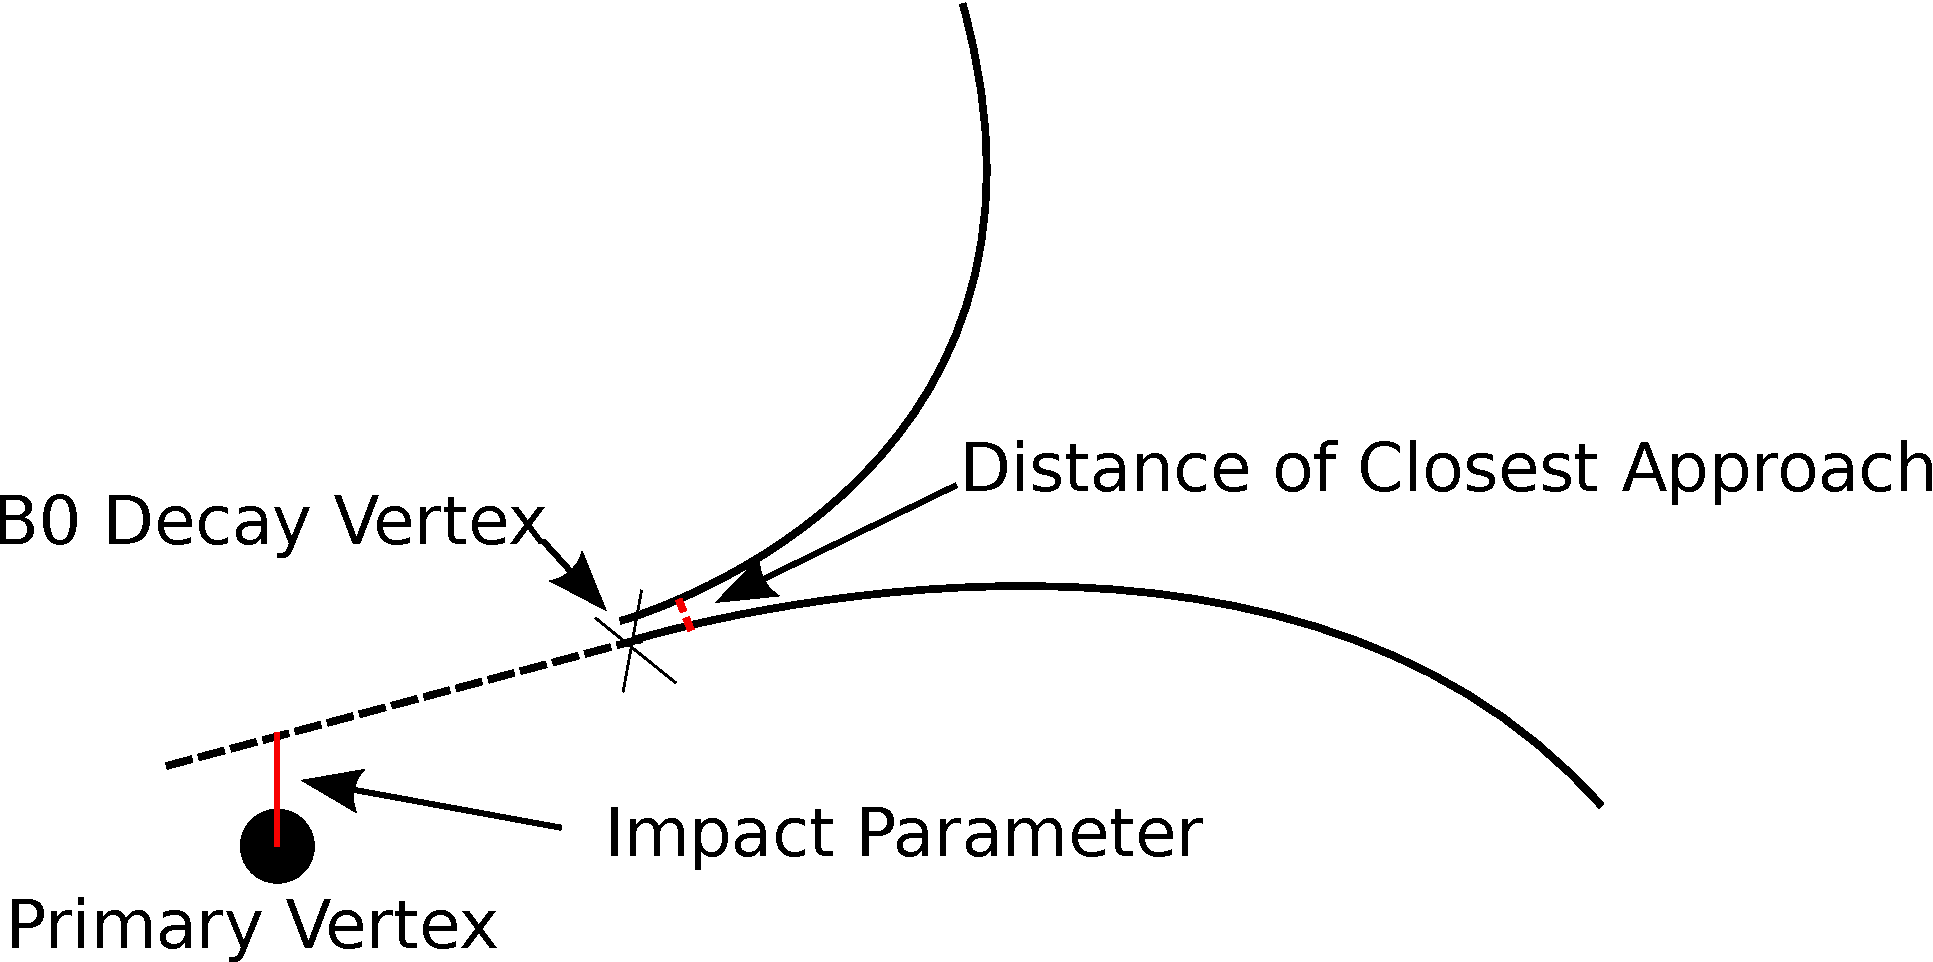
\includegraphics[width=\textwidth]{IPandDOCA.pdf}
  \caption{A schematic diagram showing DOCA and IP in a typical \Bd decay.}
  \label{fig:DOCAandIP}
\end{figure}
The efficiency of this selction can be assessed by applying it to signal MC; the efficiency is then simply $\frac{No. True Signal Events Passing Stripping}{ No. Generated}$.
%However, when the \lhcb analysis software is ran on MC not every resulting event is a true signal event.  This is because false candidates can easily be created for a variety of reasons, but the most common of which is when particles from other pp interactions in the same bunch crossing get wrongly attributed as a candidate particle.  To ensure only true MC signal events are used in this analysis truth cuts are applied before it is used.

The stripping efficiency is then found to be $0.00317 \pm 0.00002$, which is a quite typical stripping efficiency at \lhcb.

\subsubsection{Trigger}
\label{sec:trigger}
\lhcb has many trigger selections (trigger lines) that are applied as part of the triggering process, each of which is tailored towards a set of analyses with common properties. If an event passes any of these trigger lines it is stored, but the specific trigger lines that it passed are flagged.  Therefore, the next step of the analyses is to require events to pass trigger lines more specific to this analysis.

When an event passes a trigger line it can be described as triggered on signal (TOS) or triggered independent of signal (TIS).  TOS is when a candidate signal particle, or any component of the event contributing to it's reconstruction, causes the event to pass the trigger line.  More specifically, a minimum of $70\%$ of the trigger objects (e.g track, calorimeter cluster) that caused the event to pass the trigger line have to belong to the signal candidate. An event is classified as TIS if objects not used to reconstruct the signal candidate caused the caused the event to pass the trigger line \cite{1748-0221-8-04-P04022}. This TIS and TOS information can be used to perform a data driven assessment of triggering efficiencies, although this is not performed for this analysis(yet)\cite{Tolk:1701134}.

In order to pass the trigger selection, an event must satisfy the following criteria:
\textit{
  (L0GlobalTIS \textbf{OR} L0HadronDecision TOS) \textbf{AND} (Hlt1TrackAllL0Decision TOS) \textbf{AND} (Hlt2Top2BodyBBDTDecision TOS \textbf{OR} B0 Hlt2Topo3BodyBBDTDecision TOS \textbf{OR} Hlt2Topo4BodyBBDTDecision TOS)
}

The L0 Hadron Decision TOS line is required because the final state of this analysis contains 4 hadrons, therefore events that do not pass this trigger line are unlikely to be signal.  The Hlt2 trigger lines make use of the fact that this stage of the trigger is applied offline and apply a boosted decision tree (BDT) using topological variables, more description of BDTs is given in section \ref{sec:multivar}.

As part of the monte carlo production process the \lhcb trigger system is emulated, therefore MC events are also flagged with the trigger lines they pass.  This means the signal efficiecny of this trigger selection can be assessed simply by applying it to MC.  The signal efficiency of this trigger selection is found to be $0.715\pm0.006$.  This is a good trigger efficiency for \lhcb, and considerably higher than the approximately $20\%$ efficiency that hampered the analysis of \Lb \to \Lz\etaz \cite{LHCb-PAPER-2015-019}.

\subsubsection{Multivariate Selection}
\label{sec:multivar}
There are many kinematic and detector variables associated with every event that can be used to discriminate signal events from background events.  However, applying cuts to these variables individually does not provide optimal signal and background seperation.  Furthermore, there are often correlations between the variables that are difficult to account for when individual cuts are used.  For both of these reasons a multivariate selection procedure is applied in this analysis which makes use of all the available variables at the same time.  It has been seen in many other \lhcb analyses that the most effective type of multivariate analysis is a boosted decision tree(BDT).  BDT's were first developed as a way of perforiming particle identification at the MiniBooNE neutrino experiment but have since been used very widely within HEP experiments as well \cite{2005NIMPA.555..370Y}.

\paragraph{Decision Tree}
A simple decision tree (DT) is just a set of binary cuts applied one after the other to decide if an event is signal or background.  Each cut is known as a node. The positions of these cuts are chosen (trained) based on control samples of data that are known to be signal and background.  The gini index is given by, $G=P(1-P)$ where P is the purity of a subset of events.  At each node the positon of the cut is chosen to optimise the criterion C which is given by,

\begin{equation}
  C=G_{node}-G_{passing}-G_{not passing}
\end{equation}

An example of a trained DT is shown in Figure \ref{fig:DT}.  Every event in this tree has the initial selection criteria at the top of the tree applied, and then the further cuts are applied depending on the output of the first.  Every event is then classified as signal or background by this tree.

The specific tree shown in Figure \ref{fig:DT} has been used to classify artificial events just based on the variables $x$ and $y$.  Figure \ref{fig:square} shows a scatter plot of $x$ against $y$ populated by both ``signal'' and ``background'' events.  The positions of the cuts applied by this DT are also shown; it can be seen they seperate signal and background reasonably well.  If more variables are used, more nodes can be added to the decision tree and the cuts become multi dimensonial.
\begin{figure}[h]
  \centering
  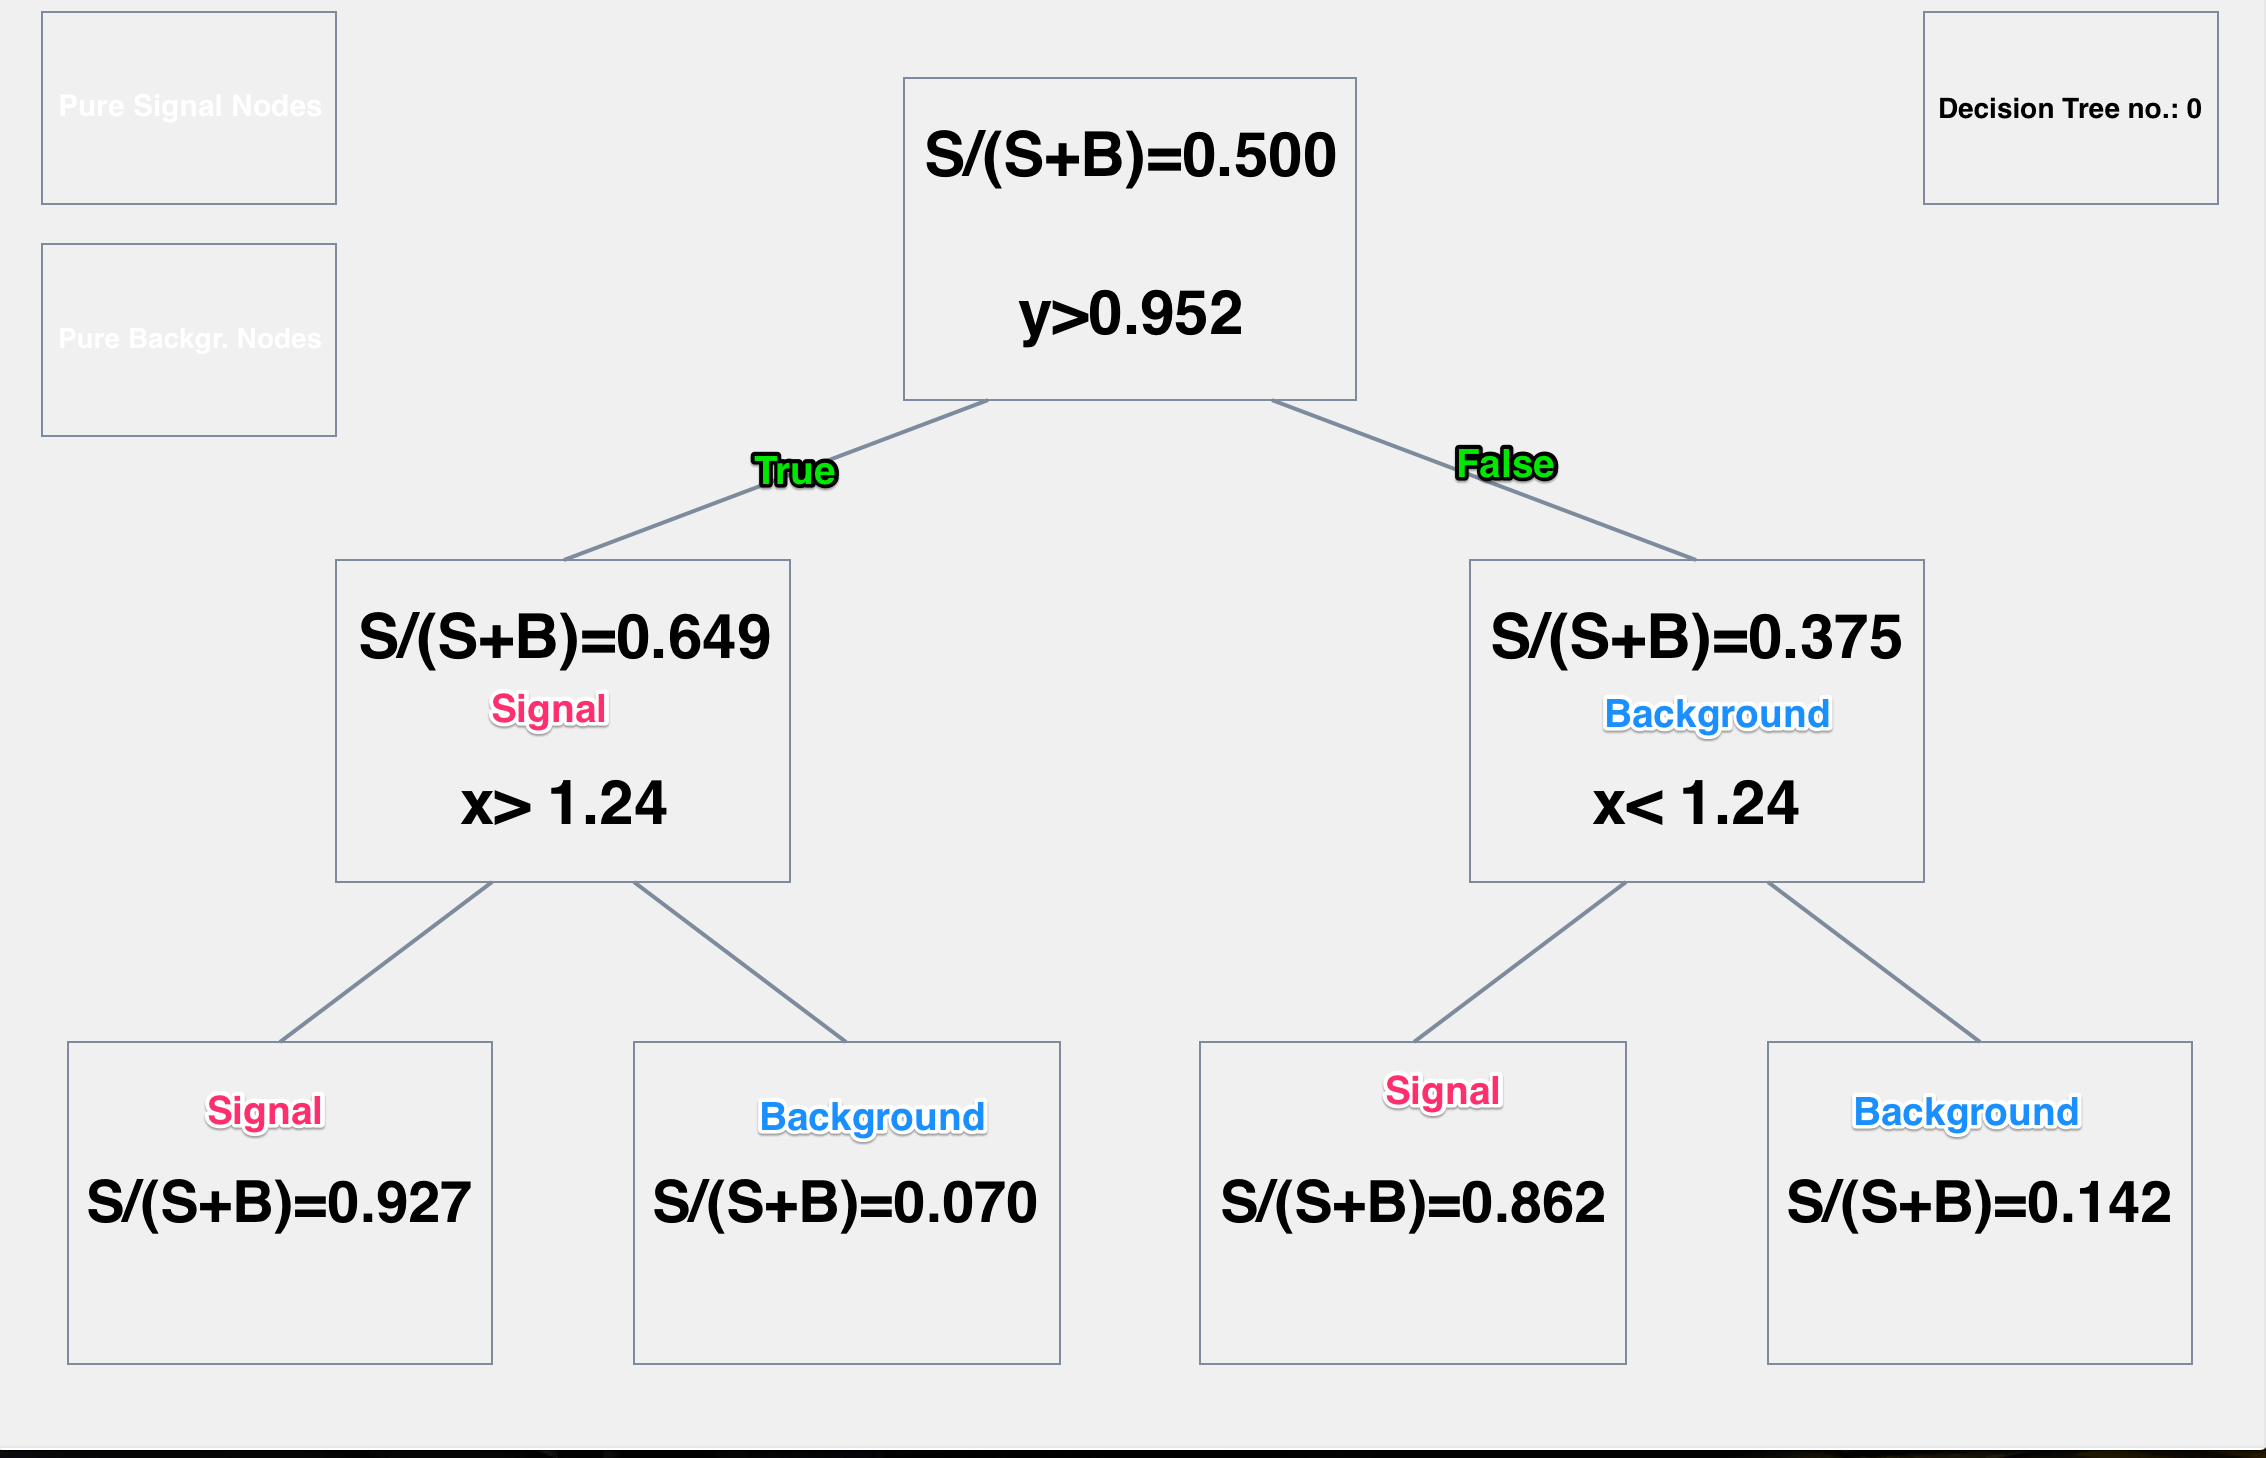
\includegraphics[width=\textwidth]{DT.png}
  \caption{A single decision tree that is classifying events as signal or background based on the artificial variables x and y}
  \label{fig:DT}
\end{figure}
\begin{figure}[h]
  \centering
  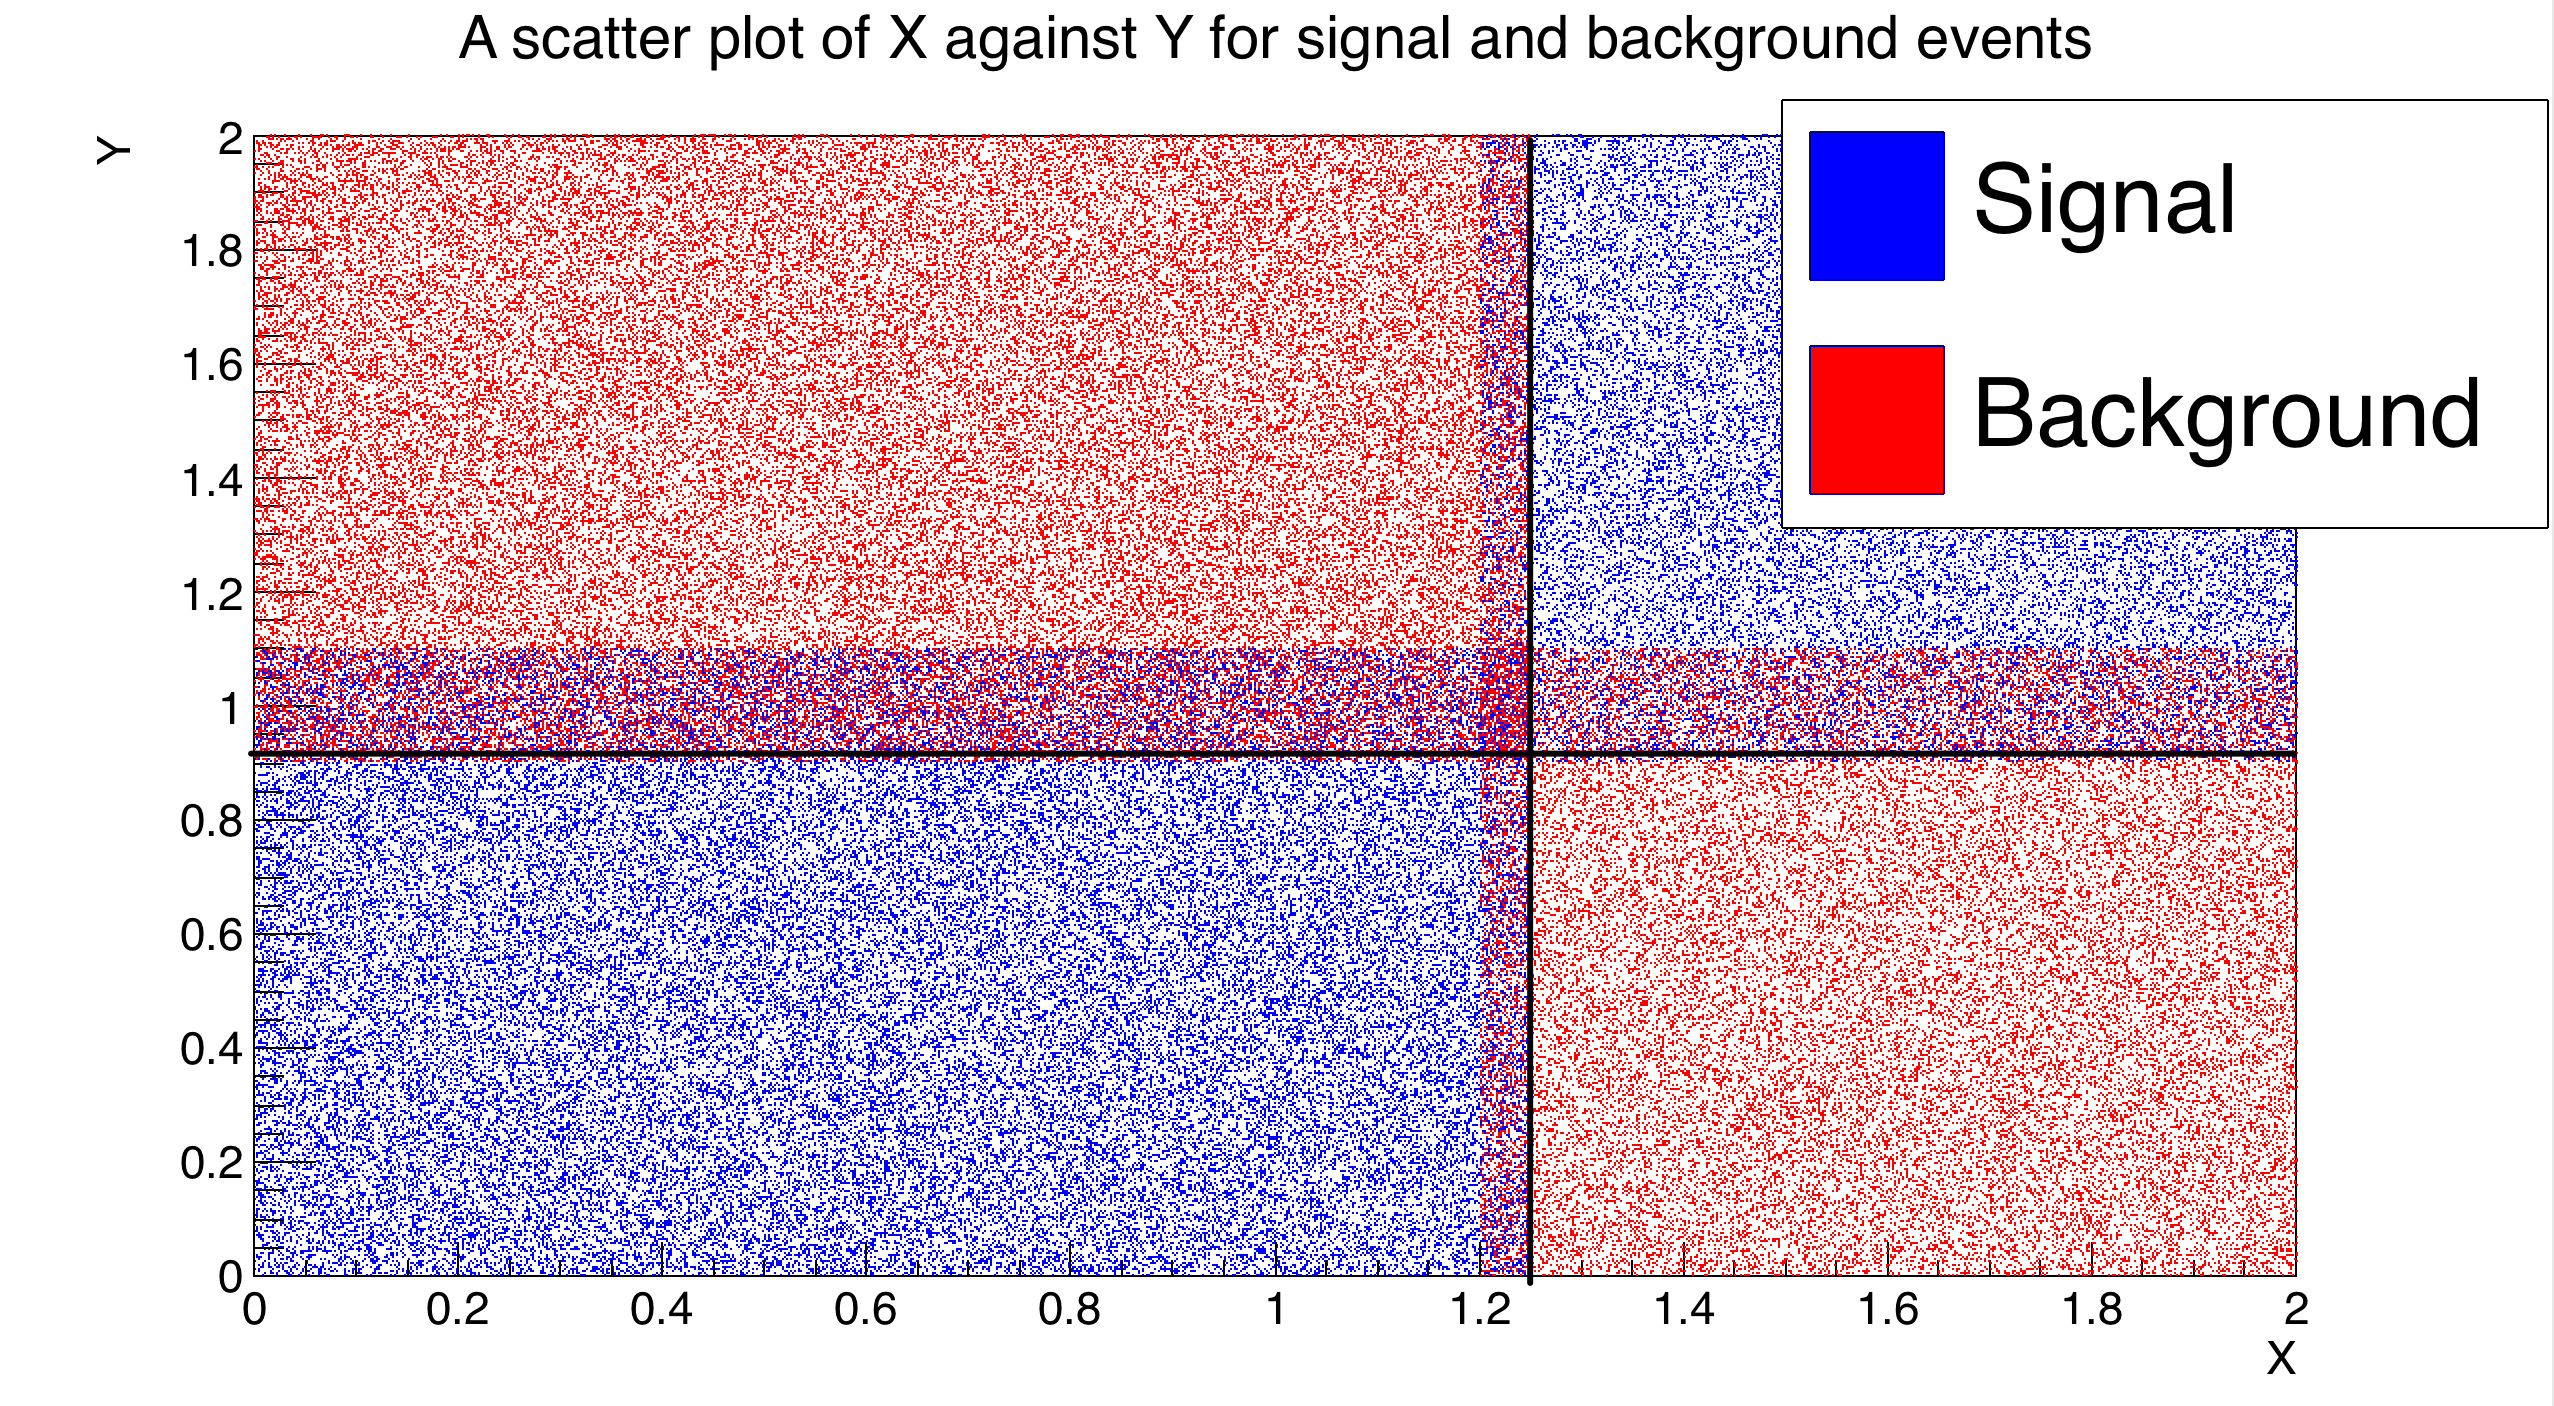
\includegraphics[width=\textwidth]{square.png}
  \caption{A scatter plot of $x$ against $y$ for the artificially generated events. The black lines show the cuts applied by the trained decision tree in Figure \ref{fig:DT}}
  \label{fig:square}
\end{figure}

It should be noted that the artificial variables provide better seperation than any found in real data but despite this there are still background events that are classified as signal events and vica versa. Also, it is not unusual for some analyses to use as many as 30 variables in a multi variate analysis which would make a single decision tree very complex.  The biggest reason why a single decision tree is not used, however, is because the training of a single tree is not stable; it is highly susceptible to statistical fluctuations.

\paragraph{Boosting}
These issues are solved by the boosting process, which involves training many decision trees (400-1200), scoring the effectiveness of the tree and returning a single value that is the weighted average of the response from all the trees.  In this analysis the TMVA package is used to train and apply BDTs which uses the Adaboost algorithm\cite{Hocker:2007ht}. 

After all the DTs are trained, the first step in the boosting process is to assign all events a weight $W=\frac{1}{m}$ where m is the number of events in the control sample.  To caluclate the score, $\alpha$, of each DT the fraction of events that are mis identified,E, is calcualted for every DT. This is another reason why control samples of known signal and background events are required for training.  A DT with a low value of E is chosen as the first DT to score and the value of $\alpha$ for that DT is calculated as,
\begin{equation}
  \alpha=\beta ln\big(\frac{1-E}{E}\big)
\end{equation}
where $\beta$ is a constant.  Next, the weights of events mis identified by the first DT are re assigned to be,
\begin{equation}
  W=W e^{\alpha}
\end{equation}
and all event weights are renormalised.  This lends more weight to mis idenitifed events. The same scoring process is then iteratively applied to every DT trained, but mis identified events are only re weighted until the total weight of all mis identified events reaches $50\%$. 

For a given event the final BDT value assigned is given by,

\begin{equation}
  V=\sum \limits_{i}^{N_{Trees}}\alpha_iV_i
\end{equation}

where $\alpha_i$ is the score assigned to the i'th decision tree and $V_i$ is the output of the $i_{th}$ decision tree which is -1 if the DT classifys the event as background and 1 if it is classified as signal.  This means the final value assigned to an event by the BDT is between -1 and 1 with 1 being more likely to be signal.  After the BDT is applied, there is a single BDT variable that can be cut on.

%TODO add adaboost reference.
\paragraph{Application for \Bd \to \Kstar \etaz}
A BDT was trained, and applied to candidates that passed the trigger and stripping selections to discriminate signal from combinatorial background.  Truth matched signal MC was used as a signal control sample and data with a refitted \Bd mass greater than 5500MeV was used as a background control sample to train the BDT.  This mass was chosen because it is far enough away from the real \Bd mass to definitely be background whilst still keeping a reasonable sample size.  Data from the lower mass sideband was not used for training as it is highly likely to contain partially reconstructed backgrounds rather than pure combinatorial background.  This would be a problem because BDTs are only effective for discriminating between two classes of events.

The variables used in the BDT are shown in Table \ref{tab:vars}.  The TMVA package ranks all input variables in order of importance based on the gini value and the number of times it is the variable in the top node of the tree.  These variables were chosen by adding all variables that could possibly discriminate signal from background and then iteratively removing the lowest ranked variables.  This was done until the lowest ranked variable still made a significant contribution to the signal and background seperation.  Care was also taken to ensure variables that are poorly modelled in MC were not used, as this could lead to false seperation.  Plots comparing a selection of these input variables in the signal and background control samples are shown in Figure \ref{fig:vars}.

\begin{table}[h]
  \label{tab:vars}
  \scriptsize
  \centering
  \begin{tabular}{|c|p{10cm}|}
    \hline
    Variable & Explanation \\ \hline
    B0 PT & Transverse momentum of \Bd candidate \\ \hline
    log(1-B0 DIRA OWNPV) & natural log of one minus the DIRA angle (see section \ref{sec:stripping}) \\ \hline
    B0 ENDVERTEX CHI2 & The $\chi^2$ of the \Bd endvertex from the least squares fit used to assign the daughters to the B0 endvertex \\ \hline
    log(B0 PVFit Chi2) & The natural logarithm of the $\chi^2$ of the fit used to refit the entire decaytree described in section \ref{sec:Decay Reconstruction} \\ \hline
    B0 eta & The pseudorapidity of the \Bd candidate \\ \hline
    B0 FD OWNPV & The flight distance of the \Bd between the primary vertex and decay vertex \\ \hline
    log(B0 TAU CHI2) & The $\chi^2$ of the \Bd lifetime. \\ \hline
    Kstar CosTheta & The cosine of the angle between the \Kstar candidates momentum in the \Bd rest frame and the \Bd momentum in the lab frame. \\ \hline
    Kstar eta & The pseudorapidity of the \Kstar \\ \hline
    piminus0 OWNPV CHI2 & The $\chi^2$ of the \pim belonging to the \etaz `vertex \\ \hline
    pi0 CosTheta & The cosine of the angle between the \piz candidates momentum in the \etaz rest frame and the \etaz momentum in the lab frame.\\ \hline
    gamma PT and gamma0 PT & The transverse momentum of the photons from the \piz \\ \hline
    log B0RF KPlusKst costheta & The logarithm of the cosine of the angle between the \Kp and the \Kstar candidate in the rest frame of the \Bd. \\ \hline
    etaRF PiPlusPiMinus0 costheta & The cosine of the angle between the \pip and \pim from the \etaz in the rest frame of the \etaz. \\ \hline
    gamma0 CL and gamma CL & The probability that the photons from the \piz are actually photons.  This is assigned by the \lhcb calorimeter system. \\ \hline
    B0 Sum Track PT & The sum of the transverse momentum for all tracks in a candiate event (\pim,\Kp,\pim,\pip). \\ \hline
    B0 Sum PCHI2 & The sum of the $chi^2$ probabilities for each track belonging to the event. \\ \hline
    B0RF KPlusPiMinus costheta & The cosine of the angle between the \Kp and \pim in the rest frame of the \Bd \\ \hline
  \end{tabular}
  \caption{The variables used in the BDT, a diagram of the decay is shown in Figure \ref{fig:decaytree}}
\end{table}

\begin{figure}[h]
  \centering
  \includegraphics[width=\textwidth]{vars.png}
  \caption{Plots of 6 of the input variables showing the seperation between signal and background they provide}
  \label{fig:vars}
\end{figure}

The overall ouptut of the trained BDT for the control samples is shown in Figure \ref{fig:BDTOut}.  Firstly, this plot shows that the BDT is able to provide good seperation between signal and background.  This plot also shows the overtraining check that TMVA performs.  Overtraining occurs when the BDT becomes too sensitive to statistical fluctuations in the input variable distributions.  In the case of overtraining, the BDT shows excellent seperation for the specific control samples used but worse seperation for the input variables in general.  TMVA checks for this by splitting the control samples in half before training, and only one half is used to train the BDT.  When the BDT is trained, it is applied to the remaining half of the control sampeles, and in the case of no overtraining the distirbution of the BDT response varaible should be the same for both halves of the control samples.  Figure \ref{fig:BDTOut} shows the BDT response distributions for both the training and test samples. These are considered to be consistent, there are no systematic disrepencies between the distributions.  The Kolomogrov-Smirnov test shown on the plot should be ignored, as internal \lhcb studies have shown this to be unreliable\cite{Grünberg:2019861}.  This trained BDT was then applied to all events that passed the stripping and trigger cuts.

\begin{figure}[h]
  \centering
  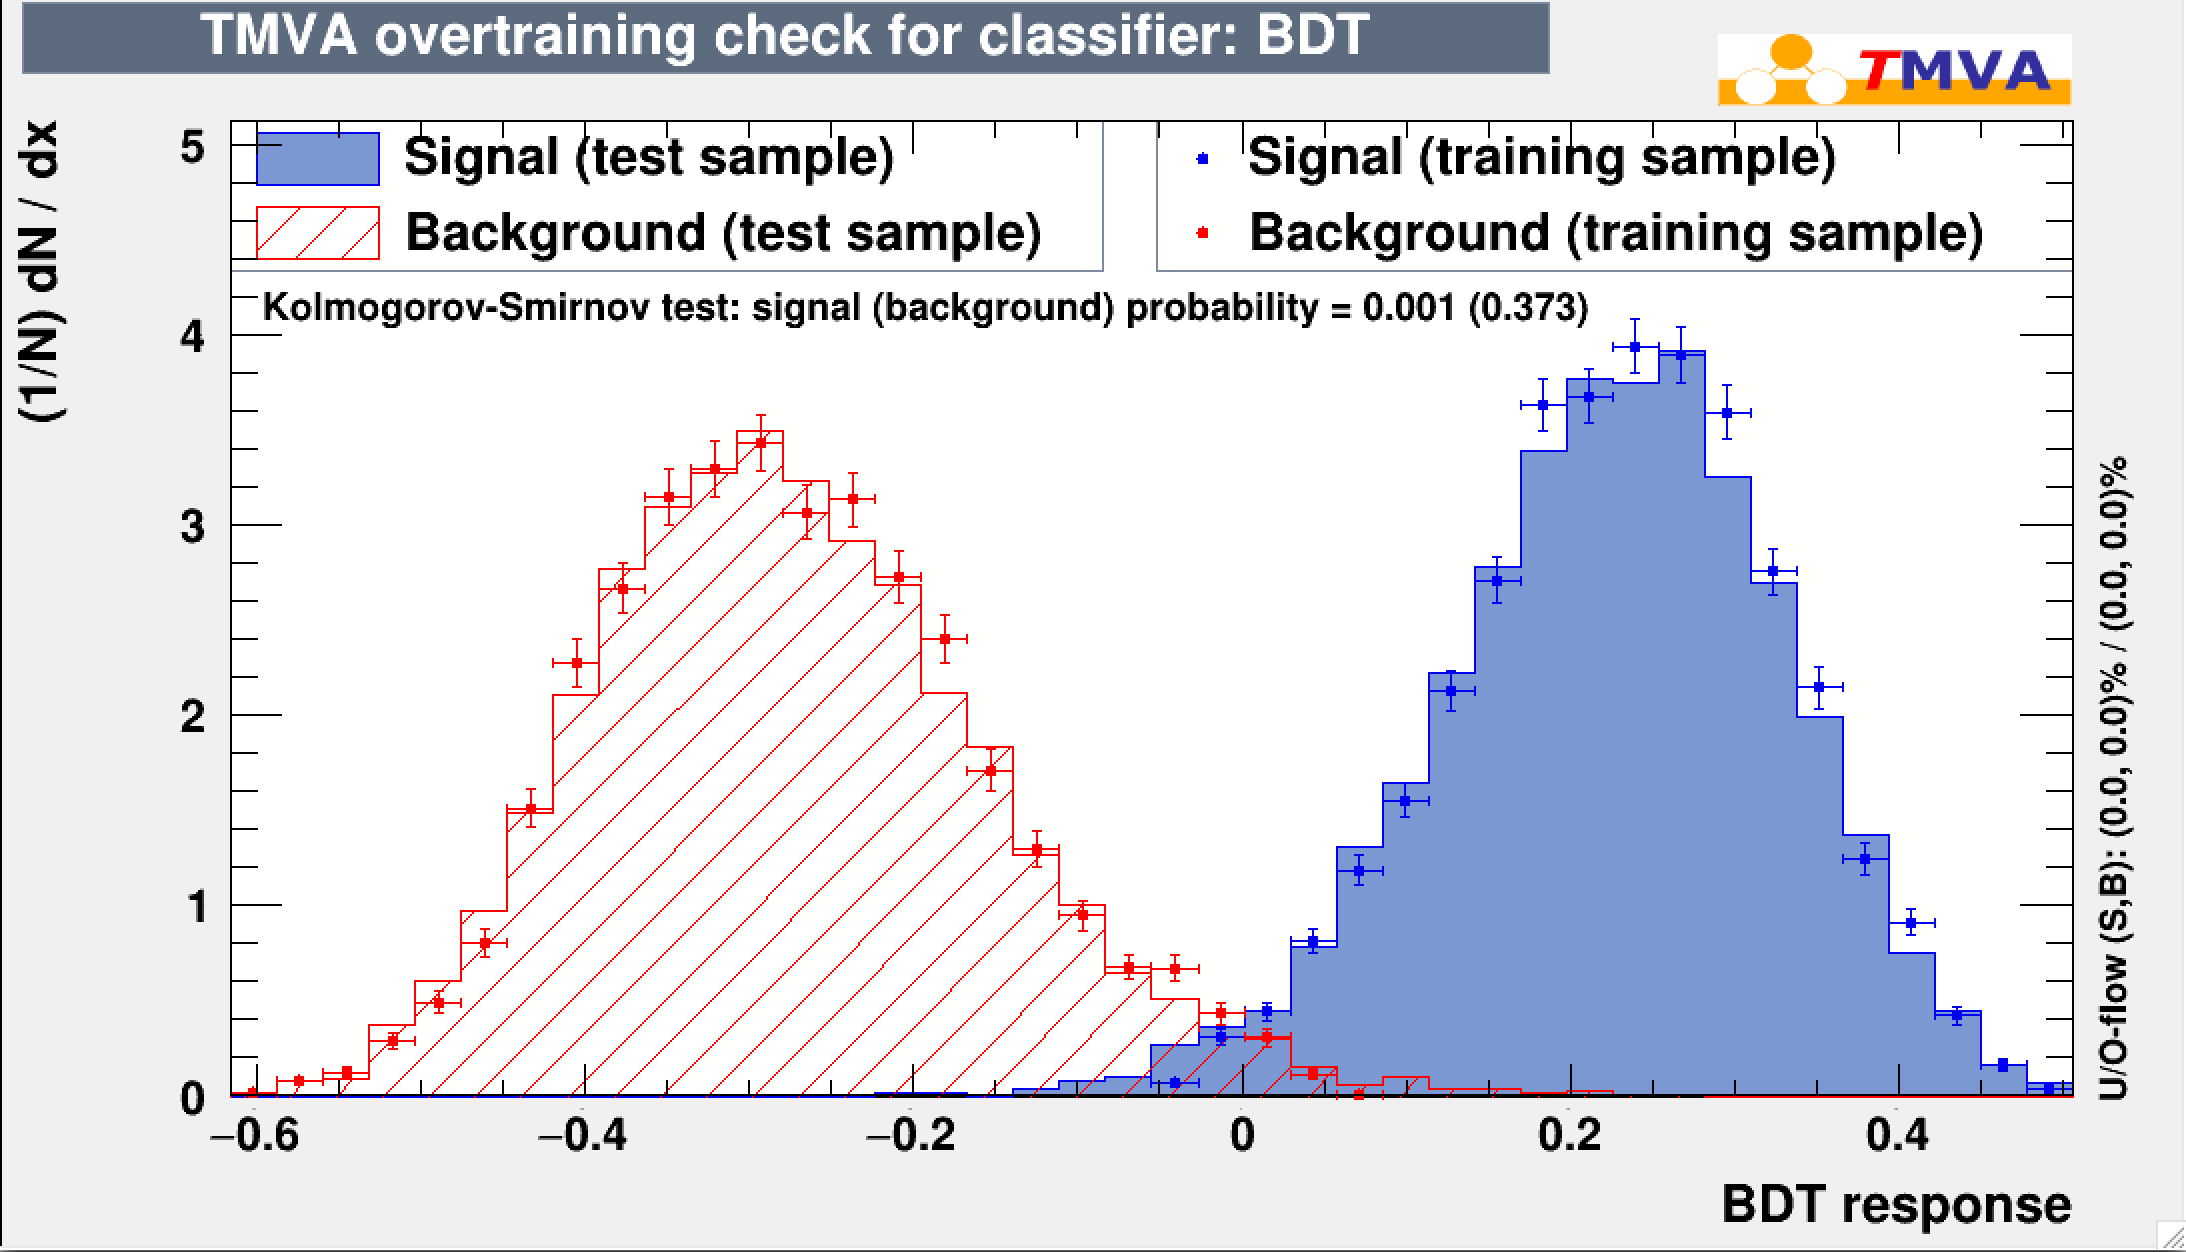
\includegraphics[width=\textwidth]{BDTOut.png}
  \caption{The output of the BDT as applied to the control samples.  This also shows the overtraining check}
  \label{fig:BDTOut}
\end{figure}
%TODO maybe do BDT double training thin

%optimisation of BDT Cut
\clearpage
\paragraph{Optimisation of BDT Cut}
A cut on the BDT response now needs to be applied.  As the \Bd meson has been observed to decay to \Kstar \etaz previously, this analysis is not performed blinded.  The consequences of this is that signal significance can be used to optimise the BDT cut.  The signal significance, $\sigma$, is defined as,
\begin{equation}
  \sigma=\frac{S}{\sqrt{S+B}}
\end{equation}
where S/B is the number of signal/background events present in a defined signal window.  The values of S and B have to be extracted with a mass fit to data at each BDT cut.

In order to paramaterise the signal shape, a mass fit to truth matched MC was first performed using Crystal Ball probability density functions(PDF).  The Crystal Ball experiment was the first to use this PDF, which is centrally a gaussian with a power law tail after a given cut off \cite{CrystallBall}.  It is a given by the function,
\begin{equation}
f(x;\alpha,n,\bar x,\sigma) = N \cdot \begin{cases} \exp(- \frac{(x - \bar x)^2}{2 \sigma^2}), & \mbox{for }\frac{x - \bar x}{\sigma} > -\alpha \\
  A \cdot (B - \frac{x - \bar x}{\sigma})^{-n}, & \mbox{for }\frac{x - \bar x}{\sigma} \leqslant -\alpha \end{cases}
\end{equation}

where
\begin{equation}
  A = \left(\frac{n}{\left| \alpha \right|}\right)^n \cdot \exp\left(- \frac {\left| \alpha \right|^2}{2}\right)
\end{equation}
\begin{equation}
  B = \frac{n}{\left| \alpha \right|}  - \left| \alpha \right|
\end{equation}
\begin{equation}
  N = \frac{1}{\sigma (C + D)}
\end{equation}
  \begin{equation}
  C = \frac{n}{\left| \alpha \right|} \cdot \frac{1}{n-1} \cdot \exp\left(- \frac {\left| \alpha \right|^2}{2}\right)
  \end{equation}
  \begin{equation}
  D = \sqrt{\frac{\pi}{2}} \left(1 + \operatorname{erf}\left(\frac{\left| \alpha \right|}{\sqrt 2}\right)\right)
  \end{equation}

  The parameter $\alpha$ describes the cut off where the function changes from a gaussian to a power law. A positive value of $\alpha$ gives a low side tail and a negative value gives a high side tail.  $\bar{x}$ is the mean of the gaussian function, $\sigma$ is the width of the gaussian and n can be interpreted as the power for the tail.  In this fit, two crystal ball functions with opposite side tails and a common mean were used.  More specifically, an extended unbinned maximum likelihood fit was used, for which the likelihood function was given by,
  \begin{equation}
    L=e^{-N_{C1}-N_{C2}}\prod_i^{D}N_{C1}C1(x_i,\alpha_1,n_1,\bar{x},\sigma_1)+N_{C2}C2(x_i,\alpha_2,n_2,\bar{x},\sigma_2)
  \end{equation}

  where $N_{c}$ is the number of signal events in each of the crystal ball functions, C1 and C2 are the two crystal ball functions with opposite side tails.  $x_{i}$ is the mass of the i'th \Bd candidate. The parameters $N_{C1}, N_{C2},\alpha_1, n_1,\bar{x}, \sigma_1, \alpha_2,n_2,\sigma_2$ are free parameters to be determined by the fit.  Practically, this was performed using the RooFit package and the MINOS method was used to determine uncertainties\cite{Verkerke:2003ir}.

  Figure \ref{fig:MCfit} shows the results of the fit performed to truth matched MC with the values of the free parameters determined by the fit.  The fit fraction in this Figure is $N_{C2}/N_{C1}$.  This shows a good quality fit to monte carlo and, crucially, it recovers the known signal yield within uncertainties.

%TODO maybe provide PULLS
  \begin{figure}[h]
    \centering
    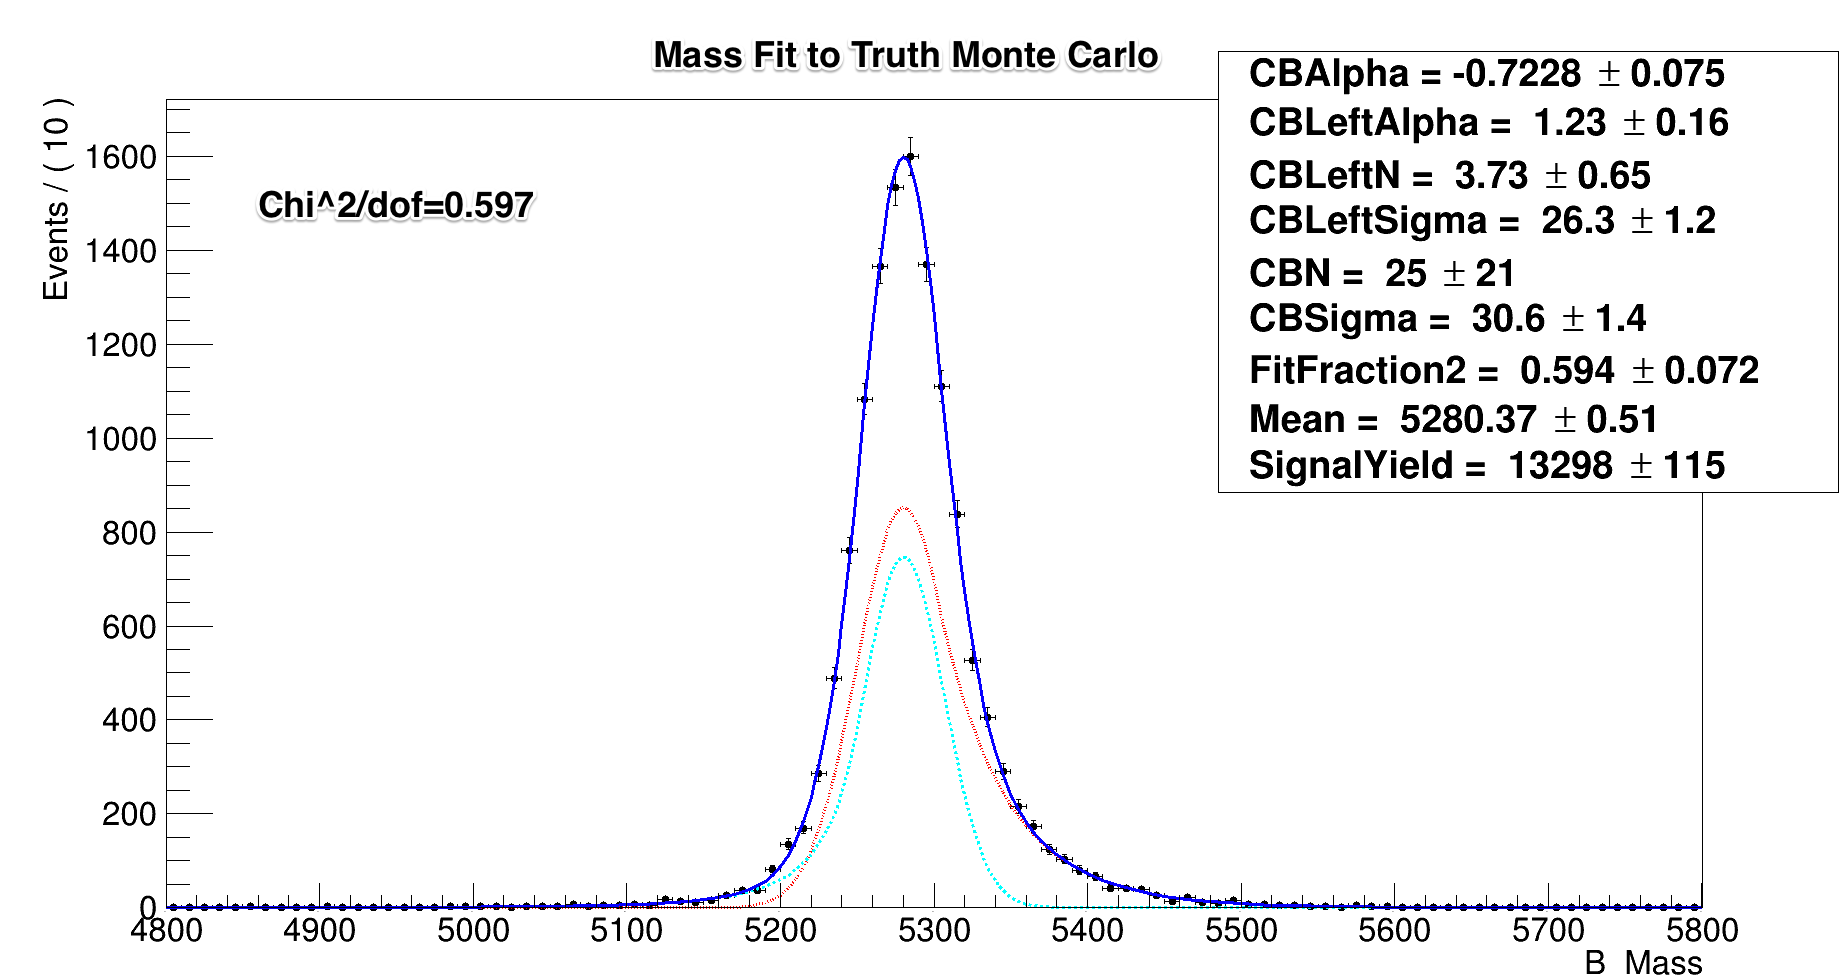
\includegraphics[width=\textwidth]{MCMassFit.png}
    \caption{A plot of the truth matched monte carlo with no BDT cut and the fitted double crystal ball function.  The red and blue dashed lines are the inidividual crystal ball functions, the solid blue line is the overall fit}
    \label{fig:MCfit}
  \end{figure}

  Now that the expected signal shape is parameterised, a mass fit to data can be carried out.  The combinatorial background was modelled with an exponential PDF, because this has described it well in analyses with similar final states\cite{LHCb-PAPER-2015-019}.  This exponential function, with its one free parameter k, was then added to the double crystal ball signal PDF.  However, for the fit to data all of the free parameters except the common mean and signal yields were fixed to those obtained in the mass fit to MC.  As these values change with BDT cut the mass fit to MC was re-performed after applying every BDT cut investigated.

  The signal window was then defined to be within $\pm2\sigma$ of the \Bd mass, and the value of $\sigma$ was taken to be the value obtained for the widest crystal ball function in the mass fit to MC. An extended unbinned maximum likelihood fit was then performed at each BDT cut and the number of signal and background events within the signal window were extracted at each BDT cut.  This allowed the signal significance as a function of BDT cut to be determined, a plot of this is shown in Figure \ref{fig:bdtsigopt}.  The uncertainty on significance was calculate by propagating through the uncertainties on signal and background yields from the fit.  Figure \ref{fig:bdtsigopt} shows that the optimum BDT cut is at a value of 0.07.  By applying the BDT to MC it is found that the signal efficiency of this cut is $0.934\pm0.008$, which is pleasingly high.

\begin{figure}[h]
  \centering
  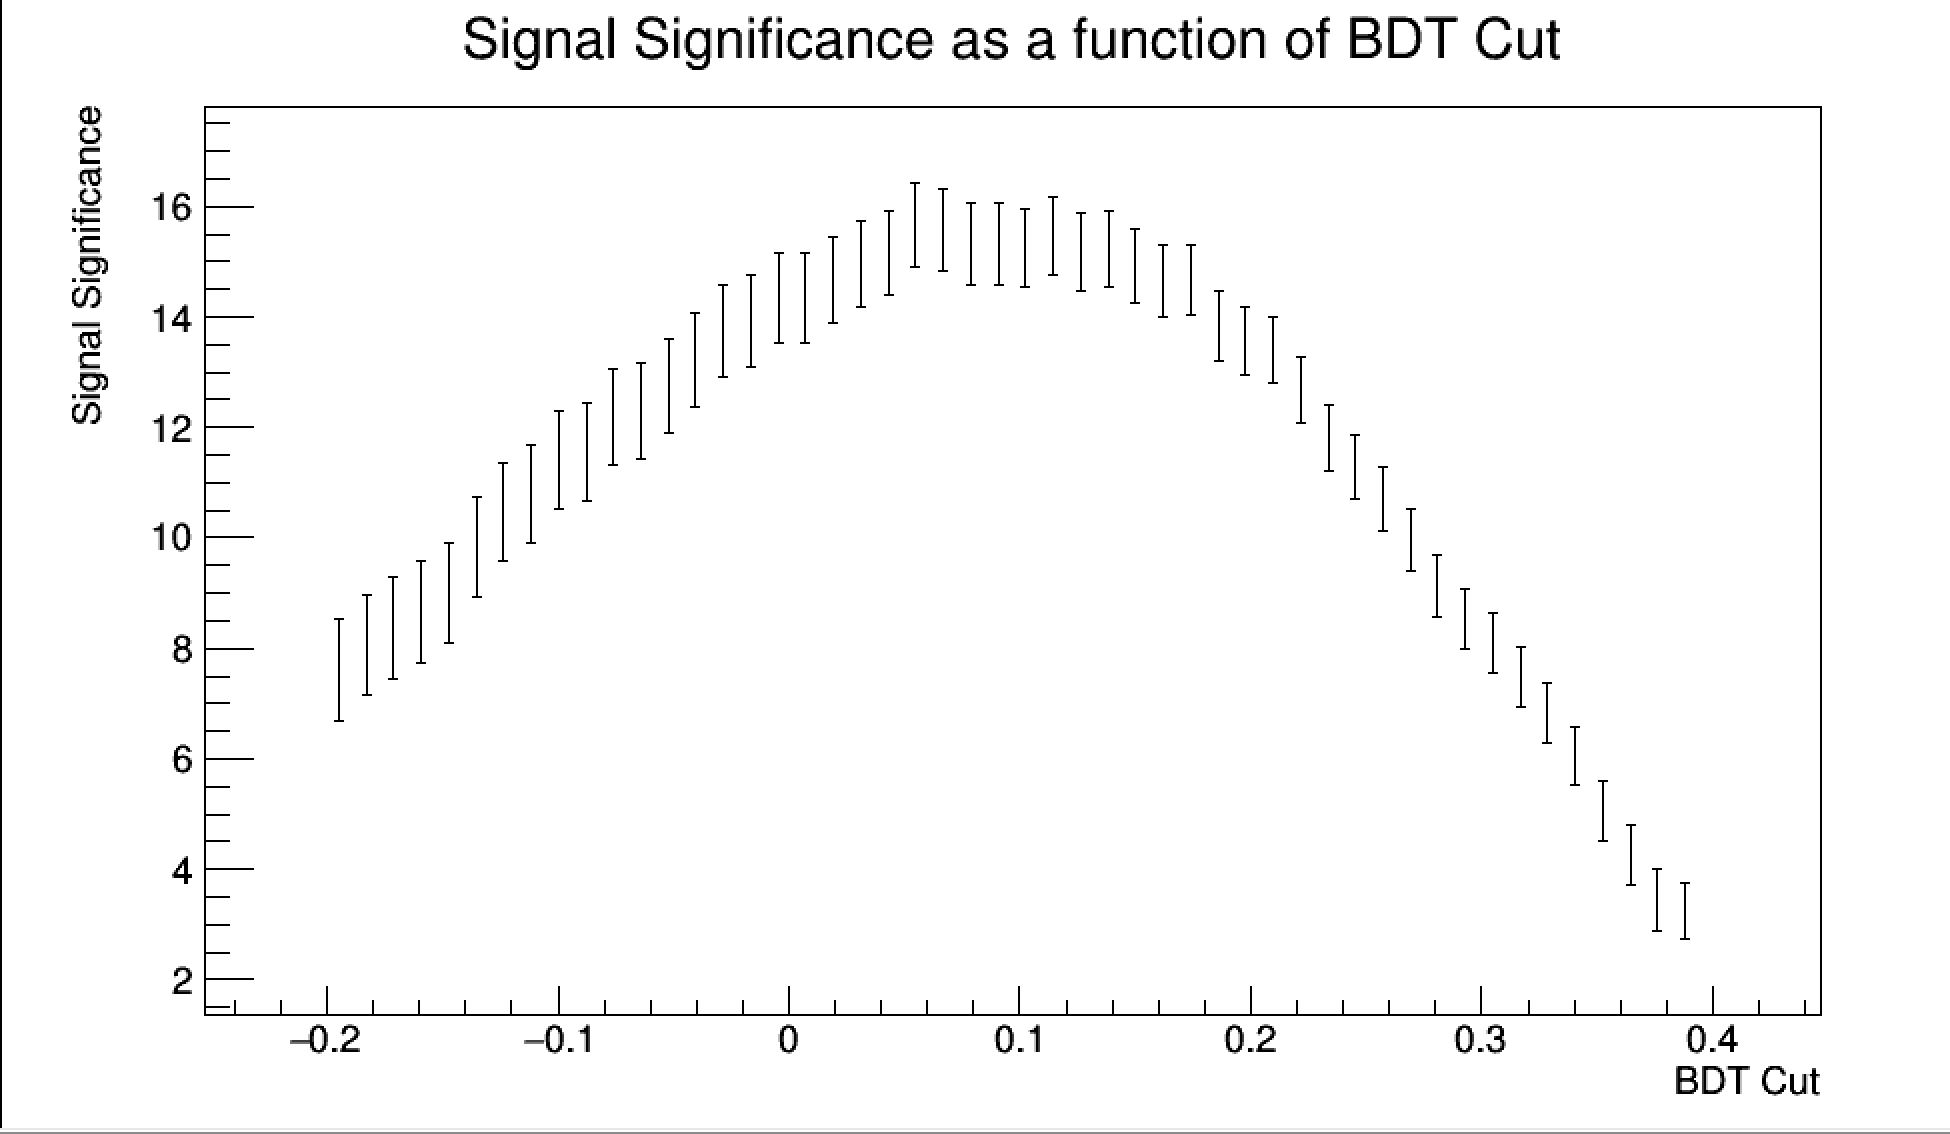
\includegraphics[width=\textwidth]{sigbdtopt.png}
  \caption{Signal significance as a function of bdt cut}
  \label{fig:bdtsigopt}
\end{figure}

Figure \ref{fig:massfit} shows the mass fit to data at this BDT cut.  Firstly the signal peak can clearly be seen with a significance of $15.9\sigma$ and a healthy signal yield of $452\pm29$ events.  However, the position of the signal peak (mean of crystal ball functions) is pulled to a higher value that is actually the limit set in the fitting procedure.  Also, there appears to be features in the background other than pure (exponential) combinatorial background which are causing data points to be systematically higher/lower than the fit in several places.  Therefore, the absolute values extracted from this fit can not be trusted, but this fit was deemed to provide an accurate enough estimate of the signal significane to optimise the BDT.  Consequently, a BDT cut of 0.07 was applied.

\begin{figure}[h]
  \centering
  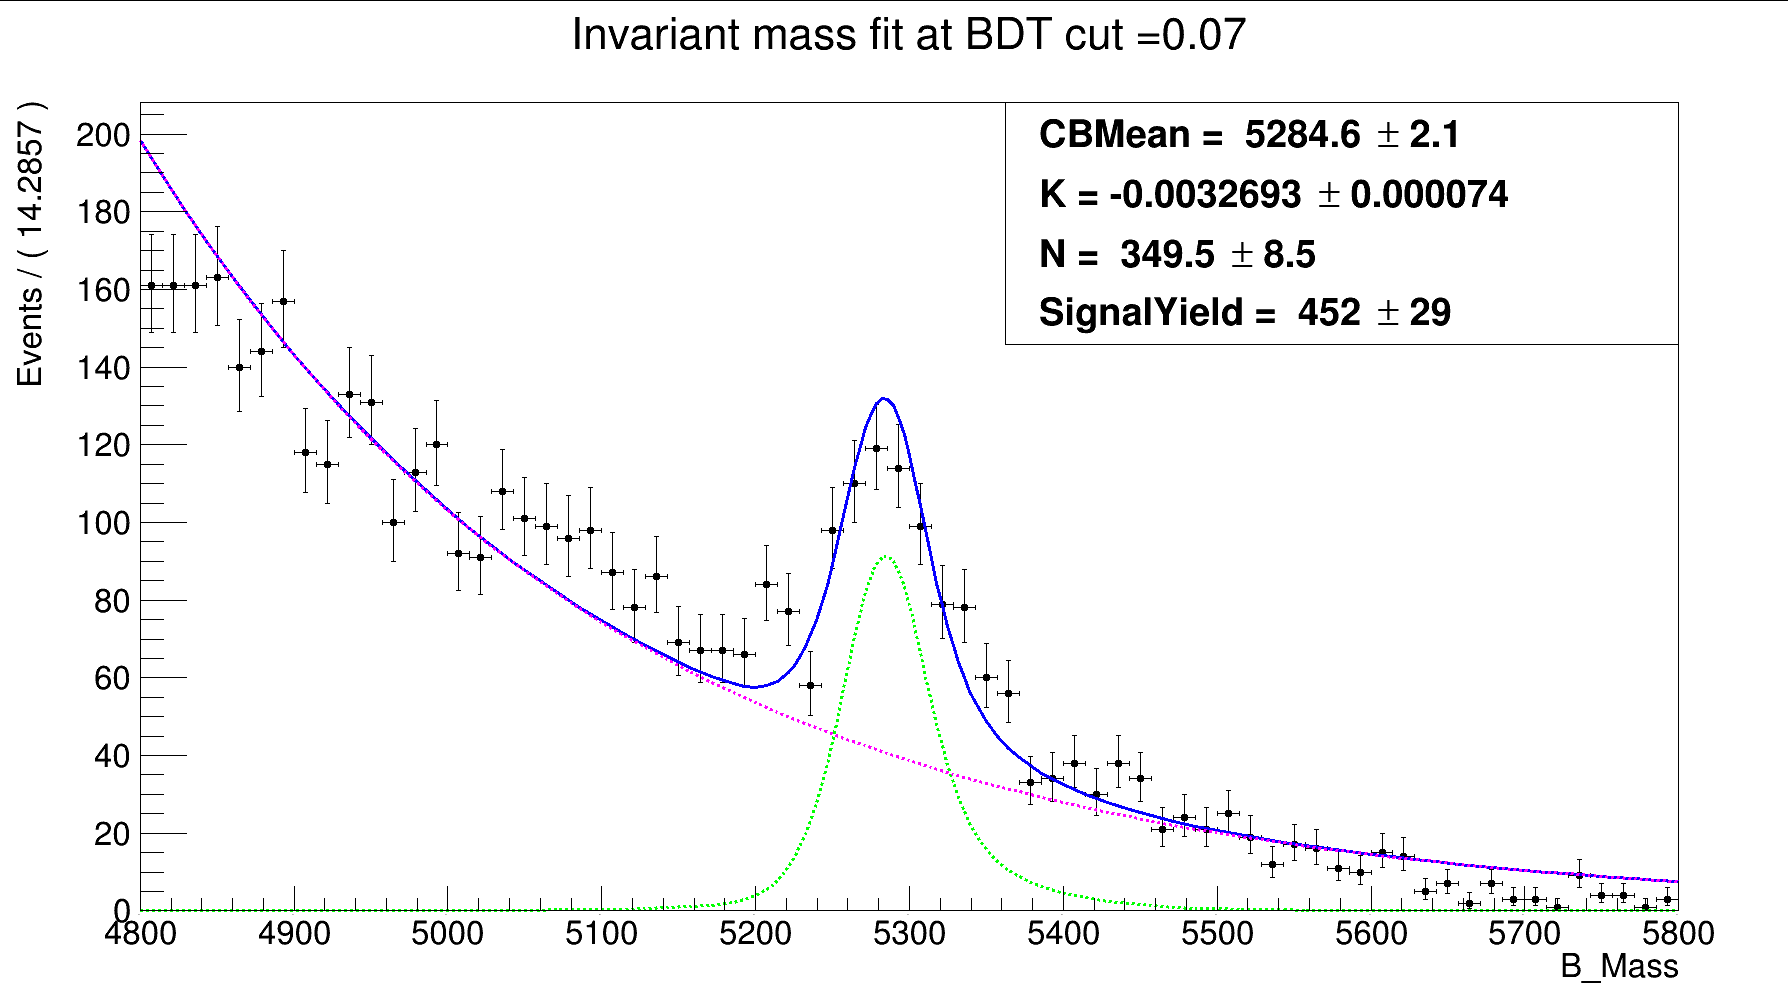
\includegraphics[width=\textwidth]{MassFit.png}
  \caption{The mass fit to data at the optimum BDT cut of 0.07.  The pink dashed line is the exponential (combinatorial) background and the green dashed line is the signal peak.  K is the constant in the exponential power, CBMean is the mean of the two crystal balls used to model signal and N/SignalYield is the number of background/signal events within the $2\sigma$ signal window.}
  \label{fig:massfit}
\end{figure}


\subsubsection{Next Steps}
\label{sec:next steps}

The next stage of the selection is a PID selection.  This uses the PID variables from the \lhcb detector to remove particles that are mis identified. However, before this can take place the features in the background that are not just combinatorial need to be understood and ideally paramaterised.  After the PID selection is complete multiple candidates need to be considered, which is when there is more than one \Bd candidate per bunch crossing.  The way multiple candidates are dealt with will be decided after they have been investigated, as they can arise in several ways. A selection can then also be developed for 2011 data and, if detector effects are the same, combined with 2012 data. A single mass fit can then be performed to extract the total signal yield in all $3fb^{-1}$ of data. This can then be used as a control channel in the search for \Lb \to p \Km \etaz.
%TODO check likelihood

%Decay Reconstruction
%Selection
%---Stripping
%---Trigger Selection
%---BDT
%---

\clearpage



\addcontentsline{toc}{section}{References}
\setboolean{inbibliography}{true}
\bibliographystyle{LHCb}
\bibliography{main,LHCb-PAPER,LHCb-CONF,LHCb-DP,LHCb-TDR}

\end{document}
